\documentclass[pmlr]{jmlr}% new name PMLR (Proceedings of Machine Learning)

% The following packages will be automatically loaded:
% amsmath, amssymb, natbib, graphicx, url, algorithm2e

%\usepackage{rotating}% for sideways figures and tables
%\usepackage{longtable}% for long tables

 % The booktabs package is used by this sample document
 % (it provides \toprule, \midrule and \bottomrule).
 % 
 % book quality tables
 \usepackage{booktabs}
 \usepackage{wrapfig}
 
 % The siunitx package is used by this sample document
 % to align numbers in a column by their decimal point.
 % Remove the next line if you don't require it.
\usepackage[load-configurations=version-1]{siunitx} % newer version
 %\usepackage{siunitx}

%hz added package
\usepackage{enumitem}
\usepackage{float}

% Avoid annoying warnings that come with some pdf figures
\makeatletter
\def\set@curr@file#1{\def\@curr@file{#1}} %temp workaround for 2019 latex release
\makeatother

\newcommand{\todo}[1]{{\color{red} #1}}
\newcommand{\mch}[1]{{\color{orange} #1}}

% change the arguments, as appropriate, in the following:
\jmlrvolume{}
\jmlryear{2023}
\jmlrworkshop{} %Machine Learning for Healthcare}

\firstpageno{1}
\usepackage{titletoc}
\usepackage{titlesec}

%%% MCH SPACE-REDUCING HACK 1/3
% Small captions
\usepackage{subcaption}
\captionsetup[table]{font=small,labelfont=small}
\captionsetup[figure]{font=small,labelfont=small}

%%%% MCH SPACE-REDUCING HACK 2/3
%% Reduce spacing around floats 
\setlength{\floatsep}{8pt plus 4pt minus 4pt}
\setlength{\textfloatsep}{8pt plus 4pt minus 3pt}

\title[Detecting Heart Disease from Multi-View Ultrasound via SAMIL]{Detecting Heart Disease from Multi-View Ultrasound Images via Supervised Attention Multiple Instance Learning}
%\title[Short Title]{Prior Guided Attention-Based Multiple Instance Learning with Self-supervised Patient Representation Learning to Detect Heart Disease in Multi-View Ultrasound Images}

\author{\Name{Zhe Huang}$^{1}$
		\Email{\textsc{zhe.huang@tufts.edu}}
\AND
        \Name{Benjamin S. Wessler}$^{2}$
		\Email{\textsc{bwessler@tuftsmedicalcenter.org}}
\AND       
        \Name{Michael C. Hughes}$^1$
        \Email{\textsc{michael.hughes@tufts.edu}}
        \\
        \addr $^1$ Dept. of Computer Science, Tufts University, Medford, MA, USA
        \\
        \addr $^2$ Division of Cardiology, Tufts Medical Center, Boston, MA, USA
}%endauthortag



\begin{document}
%%% MCH SPACE-REDUCING HACK 3/3
% Reset vertical space for equations 
% (must be after \begin{document})
\setlength{\abovedisplayskip}{2pt plus 3pt}
\setlength{\belowdisplayskip}{2pt plus 3pt}

\maketitle

\begin{abstract}
  %Incoporating Ben's feedback
Aortic stenosis (AS) is a degenerative valve condition that causes substantial morbidity and mortality. This condition is under-diagnosed and under-treated. In clinical practice, AS is diagnosed with expert review of transthoracic echocardiography, which produces dozens of ultrasound images of the heart. Only some of these views show the aortic valve. To automate screening for AS, deep networks must learn to mimic a human expert’s ability to identify views of the aortic valve then aggregate across these relevant images to produce a study-level diagnosis. We find previous approaches to AS detection yield insufficient accuracy due to relying on inflexible averages across images. We further find that off-the-shelf attention-based multiple instance learning (MIL) performs poorly. We contribute a new end-to-end MIL approach with two key methodological innovations. First, a supervised attention technique guides the learned attention mechanism to favor relevant views. Second, a novel self-supervised pretraining strategy applies contrastive learning on the representation of the whole study instead of individual images as commonly done in prior literature. Experiments on an open-access dataset and an external validation set show that our approach yields higher accuracy while reducing model size.
% Aortic stenosis (AS) is a degenerative valve condition that causes a heavy social burden. 
% In clinical practice, the best source of diagnostic information for AS is the echocardiogram, which produces dozens of ultrasound images of the heart representing different 2D views of all the heart's valves and  chambers. Only some of these views show the \todo{aortic valve}.
% To automate screening for AS, deep networks must learn to mimic a human expert's ability to identify views of the aortic valve then aggregate across these relevant images to produce a study-level diagnosis.
% We find previous approaches to AS detection yield insufficient accuracy due to relying on overly-simple averages across images. We further find that off-the-shelf attention-based multiple instance learning (MIL) performs poorly. 
% We contribute a new end-to-end MIL approach with two key methodological innovations for model training.
% First, a \todo{supervised} attention technique guides the learned attention mechanism to favor relevant views.
% Second, a novel self-supervised pretraining strategy applies contrastive learning on the representation of the whole study instead of individual images as commonly done in prior literature. 
% Experiments on an open-access dataset and a external validation set show that our approach yields higher accuracy while reducing model size.




%Moreover, our methods improves on making clinically plausible decision, which could be important in gaining trust from clinicians.

%In this paper, we develop an end-to-end solution for automating the preliminary diagnosis of Aortic Stenosis from trans-thoracic ultrasound images of the heart (echocardiograms) using an attention-based multi-instance learning (MIL) architecture. 
%Our model can take in various numbers of images from multiple view types and make a coherent diagnosis prediction for the entire study.
%Previous approaches to detecting AS require pre-filtering to specific view types by a view classifier or handle the multiple instance problem via an overly-simplistic weighted average.
%We find neither produces sufficient accuracy, 
\end{abstract}
\let\thefootnote\relax\footnotetext{Open-source Code for our Supervised Attention MIL (SAMIL): \url{https://github.com/tufts-ml/SAMIL}}

\startcontents[sections]

\section{Introduction}
\label{sec:Introduction}
%incorporating Ben's feedback
Aortic stenosis (AS) is a progressive degenerative valve condition that is the result of fibrotic and calcific changes to the heart valve. These structural changes occur over years and eventually lead to obstruction of blood flow, symptoms and death if not treated. AS is common and affects over 12.6 million adults and causes an estimated 102,700 deaths annually. AS can be effectively treated when it is identified in a timely manner though diagnosis remains challenging~\citep{yadgir2020global}. One promising route to improving AS detection is to consider automatic screening of patients at risk using cardiac ultrasound. Automatic screening could provide a systematic, reproducible process and augment current approaches that rely on cardiac auscultation and miss a significant number of cases~\citep{gardezi2018cardiac}.

% Aortic stenosis is an important valve disease.
% \todo{Explain it impacts million people over age 65}
% \todo{Explain it is easily treatable, but difficult to detect.}

% One promising route to improving detection of AS is to consider automatic screening of all routinely-collected transthoracic echocardiograms (TTEs). 
% Automatic screening could provide a systematic, reproducible process and augment current manual screening known to have inter-rater reliability issues.


\begin{figure}[!t]
\begin{tabular}{c c c}
\begin{minipage}{.45\textwidth}
(a) Human expert approach
\end{minipage}
& &
\begin{minipage}{.45\textwidth}
(b) Filter then Average {\scriptsize \citep{holste2022automated}}
\end{minipage}
\\
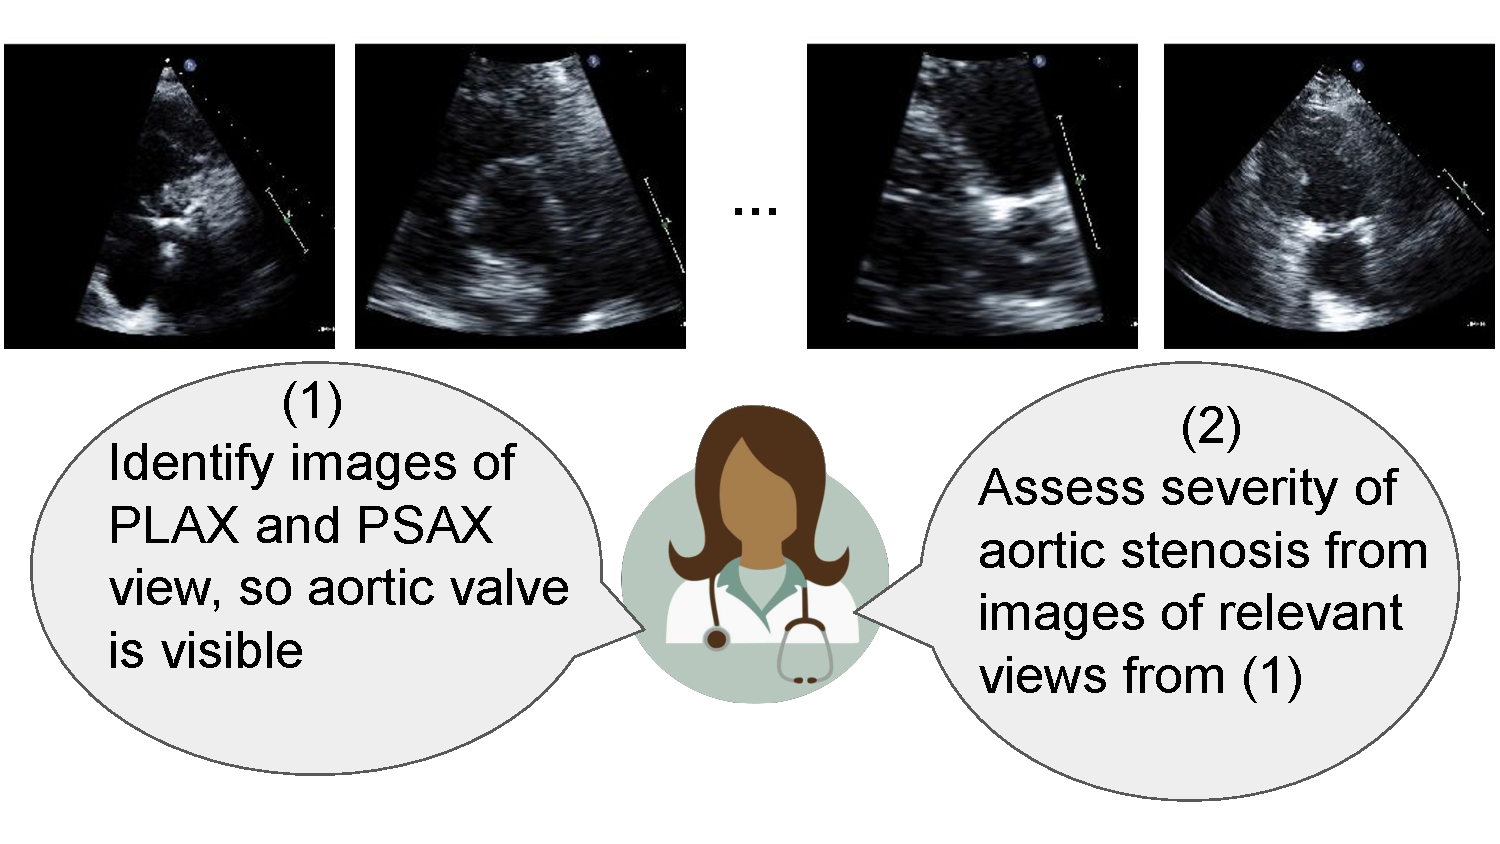
\includegraphics[width=0.45\textwidth]{figures/MIL_for_AS_diagram_1.pdf}
& &
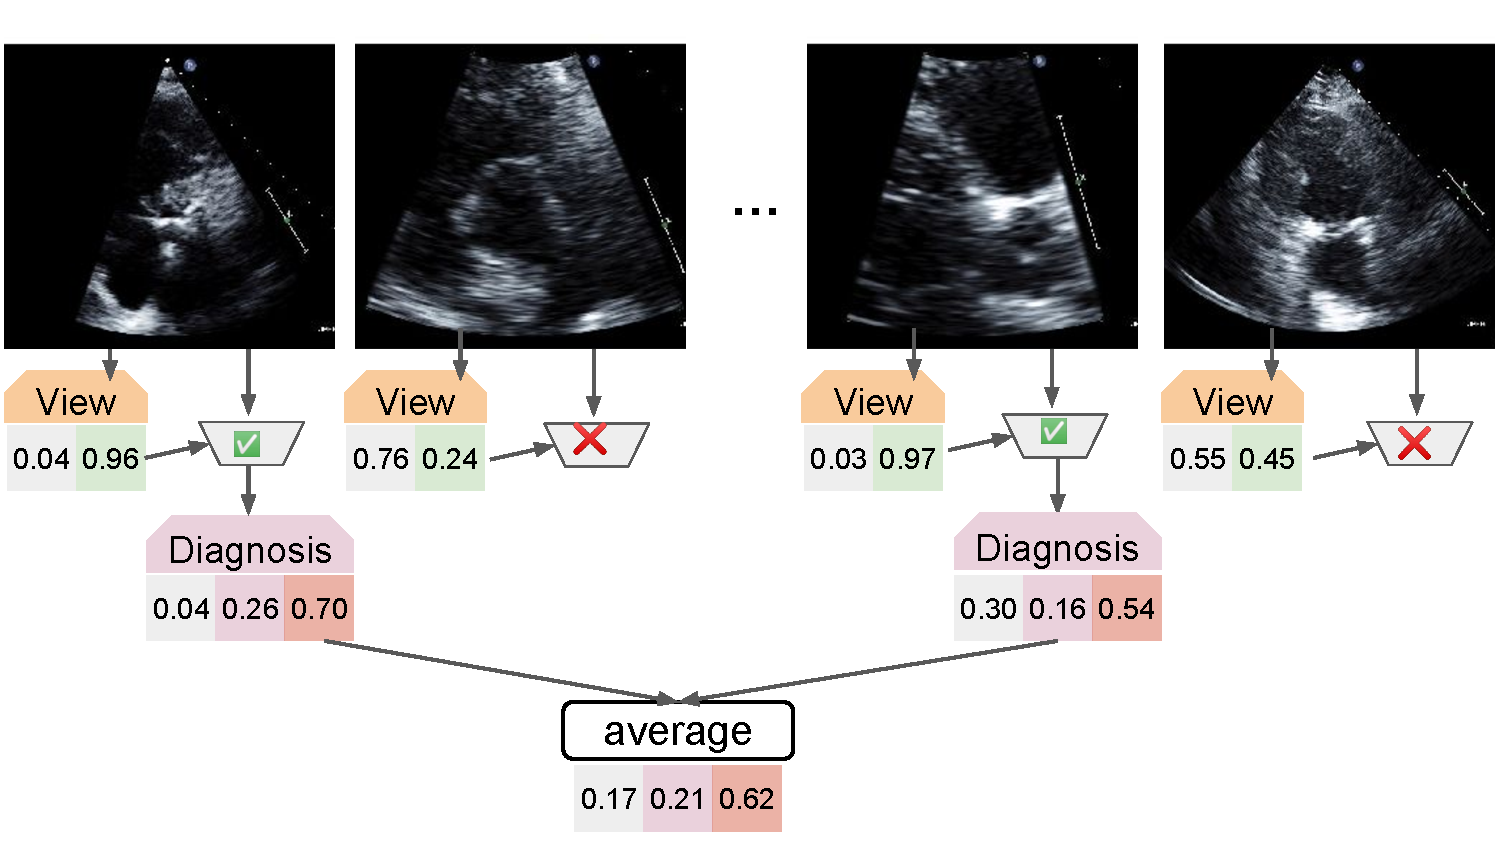
\includegraphics[width=0.45\textwidth]{figures/MIL_for_AS_diagram_2.pdf}
\\
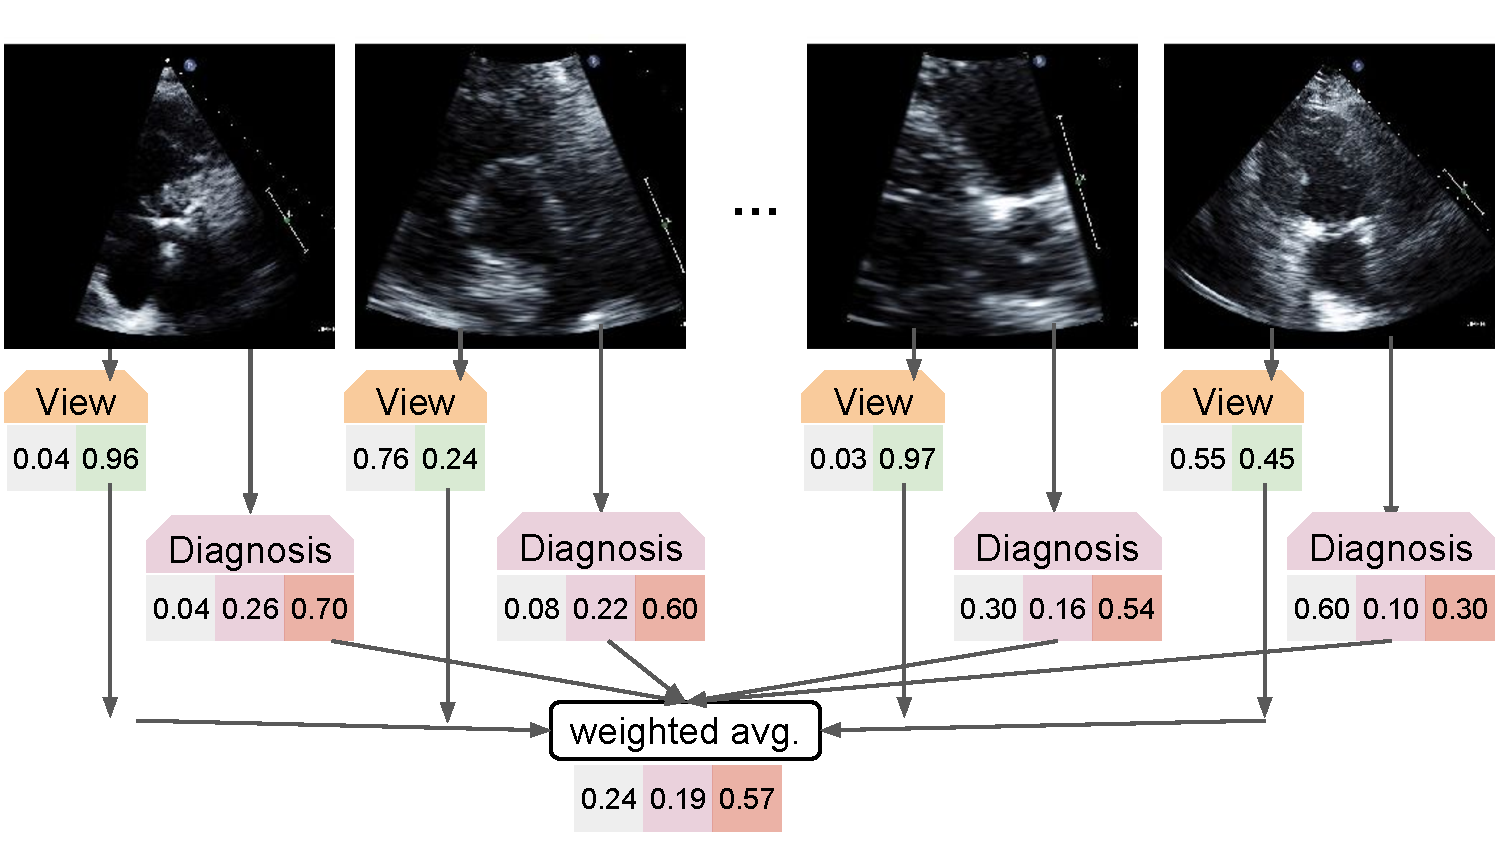
\includegraphics[width=0.45\textwidth]{figures/MIL_for_AS_diagram_3.pdf}
& &
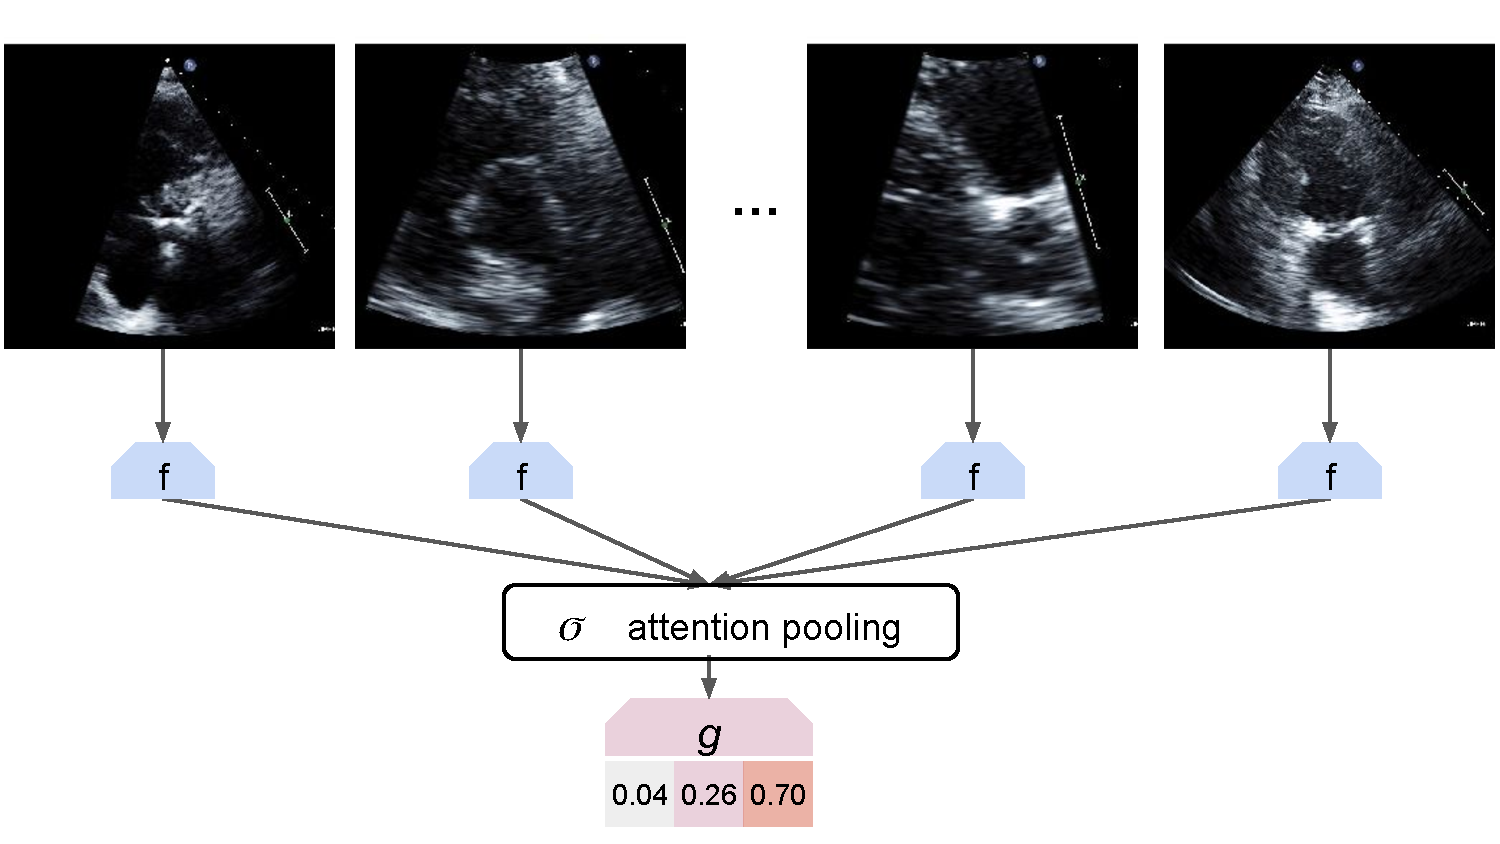
\includegraphics[width=0.45\textwidth]{figures/MIL_for_AS_diagram_4.pdf}
\\
\begin{minipage}{.45\textwidth}
(c) Weighted Average by View Relevance {\scriptsize \citep{wessler2023automated,huang2021new}}
\end{minipage}
& &
\begin{minipage}{.45\textwidth}
(d) Attention-based MIL ~\\
\end{minipage}
\end{tabular}
\caption{\textbf{Overview of methods for diagnosing aortic valve disease from multiple images of the heart.}
In our chosen diagnostic problem, the input is multiple ultrasound images representing different canonical view types of the heart's complex anatomy (e.g. PLAX, PSAX, A2C, A4C, and more, see \citet{mitchell2019guidelines} for a taxonomy).
The required output is a (probabilistic) prediction of the severity of Aortic Stenosis (AS), on a 3-level scale of no / early / significant disease.
We wish to develop deep learning methods that can solve this problem like expert cardiologists (panel a).
Two recent efforts (panel b by others, panel c by our group) made progress using a separately-trained view type classifier and per-image diagnosis classifier, but rely on combining diagnosis probabilities across images via average pooling that cannot learn how to distribute attention non-uniformly among images of relevant views.
In this work, we develop more flexible attention-based multiple instance learning architectures (MIL, panel d), with crucial contributions of supervised attention (Sec.~\ref{sec:methods_SA}) and improved pretraining strategies (Sec.~\ref{sec:methods_CL}) that we show later yield substantially improved performance on this task.
}%endcaption
\label{fig:diagrams}
\end{figure}

The challenge in developing a robust automated system for diagnosing AS is that echocardiogram studies consist of dozens of images or videos that show the heart’s complex anatomy from many different acquisition angles. As illustrated in Fig.~\ref{fig:diagrams} (a), clinical readers are trained to look across many images to identify those that show the aortic valve at sufficient quality and then use these “relevant” images to assess the valve’s health. Training an algorithm to mimic this expert human diagnostic process is difficult. Most standard deep learning classifiers are designed to consume only one image and produce one prediction. Automatic screening of echocardiograms requires the ability to make one coherent prediction from \emph{many} images representing diverse view types. To make matters more difficult, each image’s view type is not recorded in the EHR during routine collection.

% The challenge is that an echocardiogram study consists of dozens of images or videos that show the heart's complex anatomy from many different acquisition angles.
% Clinical readers are trained to look across many images to identify those that show the aortic valve at sufficient quality and then use these ``relevant'' images to assess the valve's health. Training an algorithm to mimic this expert human diagnostic process is difficult.
% Most standard deep learning classifiers are designed to consume only one image and produce one prediction. Automatic screening of echocardiograms requires the ability to process \emph{many} images representing diverse view types. Each image's view type is not stored in the EHR during routine collection.

Multiple-instance learning (MIL) is a branch of weakly supervised learning in which classifiers can consume a variable-sized set of images to make one prediction.
Recent impressive advances in MIL have been published ~\citep{ilse2018attention, lee2019set, sharma2021cluster, shao2021transmil}. 
However, their success on ultrasound tasks, especially those with images from many possible view types, has not been carefully evaluated.

% Our approach does not require the separately-trained filtering step (Fig.~\ref{fig:diagrams} (b)) for selecting relevant views for diagnosis needed by some previous AS screening methods~\citep{holste2022automated}.
\subsection*{Contributions to clinical translation and MIL methodology}
This study's contribution to applied clinical research is the development and validation of a new deep MIL approach for automatic diagnosis of heart valve disease from multiple ultrasound images produced by a  routine trans-thoracic echocardiogram (TTE) study. 
Our end-to-end approach can take as input any number of images from various view types. Our approach eliminates the need for a separately-trained filtering step (Fig.~\ref{fig:diagrams} (b)) to select relevant views for diagnosis, as required by some prior AS screening methods ~\citep{holste2022automated}. Our approach is also more flexible and data-driven than the weighted average (Fig.~\ref{fig:diagrams} (c)) of other previous efforts of AS screening~\citep{huang2021new,wessler2023automated}.
Head-to-head evaluation in Sec.~\ref{sec:Results} demonstrates that our approach can yield superior balanced accuracy for assigning AS severity grades to new studies, while keeping model size over 4x smaller than previous efforts like \citep{holste2022automated}.
Small model sizes enable faster predictions and ease portability to new hospital systems.

Our approach's success is made possible by two methodological contributions. % MIL research. 
First, we propose a supervised attention mechanism (Sec.~\ref{sec:methods_SA}) that steers focus toward images of relevant views, mimicking a human expert.
On our AS diagnosis task, supervised attention yields notable gains -- balanced accuracy jumps from 60\% to over 70\% -- over previous off-the-shelf attention-based MIL~\citep{ilse2018attention}.
Second, we introduce a self-supervised pretraining strategy (Sec.~\ref{sec:methods_CL}) that focuses contrastive learning on the embedding of an entire study (a.k.a. the embedding of the ``bag'', using MIL vocabulary). In contrast, most previous pretraining focuses on representations of individual images.
Both innovations are broadly applicable to other MIL problems involving imaging data of multiple view types.
%we introduce a novel self-supervised pretraining strategy that contrasts the bag-level embedding instead of image-level embedding, which are shown to be more effective for our problem (might also be suitable for other MIL problem).

%This study makes three contributions towards the automatic diagnosis of Aortic Stenosis using machine learning. Firstly, we propose an end-to-end multi-instance-learning approach that can diagnose Aortic Stenosis in realistic clinical scenarios, consuming various numbers of images from different view types in a realistic TTE study, without requiring pre-filtering. Secondly, we leverage clinical insights and introduce a supervised attention mechanism that uses predicted view relevance to guide the model's attention, significantly improving the performance of off-the-shelf MIL algorithms. Thirdly, we propose a novel self-supervised pre-training strategy that contrasts the bag-level embeddings, instead of the image-level embeddings, which we demonstrate to be more effective for our problem and may also be suitable for other MIL problems.

\subsection*{Generalizable Insights about Machine Learning in the Context of Healthcare}

This study offers critical insight into how multiple-instance learning can be applied to routine echocardiography studies. We show that recent MIL architectures are insufficient in achieving competitive performance and lack the ability to make \textbf{clinically plausible} decision (they attends to irrelevant instances). Our two innovations -- supervised attention (Sec. \ref{sec:methods_SA}) and bag-level self-supervised pretraining (Sec.~\ref{sec:methods_CL}.) can be broadly applicable to many clinical image analysis problems that require non-trivial aggregation over multiple images from multiple acquisition angles (views) to make one diagnosis. Beyond echocardiography, these insights could be useful for lung ultrasound, fetal ultrasound, head CT, and more.
%all of which require the clinical expert to aggregate information across multiple images from multiple acquisition angles (views).



\section{Related Work}
\label{sec:RelatedWork}

\subsection{Multiple-instance learning.}
Multiple-instance learning~\citep{dietterich1997solving,maron1997framework} describes a type of problem where an unordered bag of instances and their corresponding bag label are provided as input, and the goal is to predict the bag label for unseen bags. 
This type of problem appears in many medical applications, including whole-slide image (WSI) analysis in pathology~
\citep{cosatto2013automated,shao2021transmil,li2021dual},
% MCH trimmed
%\citep{cosatto2013automated, xu2014weakly, kandemir2015computer, zhu2017deep, campanella2019clinical, borowa2020classifying, sharma2021cluster, shao2021transmil, lu2021data, li2021dual, rymarczyk2023protomil}. 
diabetic retinopathy screening ~\citep{quellec2012multiple, li2021deep, li2021multi, kandemir2015computer}, bacteria clones identification ~\citep{borowa2020classifying}, drug activity prediction~\citep{dietterich1997solving, zhao2013drug}, and cancer diagnosis ~\citep{campanella2019clinical, chikontwe2020multiple, hou2016patch, ding2012breast, xu2014weakly}. 
Extensive reviews of the MIL literature are available~\citep{zhou2004multi, quellec2017multiple,carbonneau2018multiple}.
%% MCH trimmed: kandemir2015computer was used twice in same paragraph



Two primary ways for modeling multiple instance learning problems are the instance-based approach and the embedding-based approach. In the instance-based approach, an instance classifier is used to score each instance, and a pooling operator is then used to aggregate the instance scores to produce a bag score. In the embedding-based approach, a feature extractor generates an embedding for each instance, which is then aggregated into a bag-level embedding. A bag-level model is subsequently employed to compute a bag score based on the embedding. The embedding-based approach is argued to deliver better performance than the instance-based approach~\citep{wang2018revisiting}, but at the same time harder to determine the key instances that trigger the classifier~\citep{liu2017detecting}. 
% MCH: moved dual-stream to the next parag

% \paragraph{Classic approaches.}
% % Numerous studies have been conducted on MIL even before the  ``deep learning era'' \footnote[1]{It is usually refered to 2012 when AlexNet achieved a significant improvement in image recognition accuracy over previous methods in the ImageNet Large Scale Visual Recognition Challenge}. 
% % Numerous studies on MIL have been conducted even prior to the advent of deep learning. 
% Examples of classic MIL methods includes iARP~\citep{dietterich1997solving}, 
% Diverse Density~\citep{maron1997framework}, 
% Citation-kNN~\citep{wang2000solving}, MI-Kernels~\citep{zhang2001dd}, MI/mi-SVM~\citep{andrews2002support}, mi-Graph ~\citep{zhou2009multi}, MILBoost~\citep{zhang2005multiple}, among others. 

% Classic approaches toward multiple-instance learning are limited in the choice of $f$. For example, using pre-computed features as the representation of each instance~\citep{dietterich1997solving}or using only fully-connected layers as $f$~\citep{wang2018revisiting} for feature extraction. The choice of $\sigma$ (using restricted and very often non-trainable pooling functions such as mean pooling or max pooling ~\citep{feng2017deep, pinheiro2015image, zhu2017deep}.) 


% ~\cite{pappas2014explaining} proposed an attention-based MIL method where the attention weights are learned from an auxiliary linear regression model. 

\paragraph{Deep attention-based MIL.} 
Our proposed method builds upon recent works advancing attention-based deep neural networks for MIL. (A broader summary of classic MIL can be found in App~\ref{app:relatedworks}).
ABMIL~\citep{ilse2018attention} is an embedding approach where a two-layer neural network computes attention weights for each instance, with the final representation formed by averaging over instance embeddings weighted by attention.
Set Transformer~\citep{lee2019set} proposed to model the interactions among instances by using self-attention with multi-head attention~\citep{vaswani2017attention}. Similarly, TransMIL ~\citep{shao2021transmil} uses a Transformer-based architecture to capture correlations among patches for whole-slide image classification. C2C~\citep{sharma2021cluster} divides patches from a whole-slide image into clusters, and sample multiple patches from each cluster for training. 
C2C then tries to guide attention weights to be similar to a predefined uniform distribution, aiming to minimize intra-cluster variance for patches from the same cluster. A recent method called DSMIL~\citep{li2021dual} attempts to benefit from instance-based and embedding-based approaches via a dual-stream architecture. The author pretrains the \textbf{instance-level} feature extractor using self-supervised contrastive learning.  
%It also uses KL divergence to guide the attention weights, but different from ours, the KL-divergence is computed between the attention weights and the predefined uniform distribution, aiming to minimize intra-cluster variance for patches from the same cluster. 

%DSMIL~\citep{li2021dual} solves WSI classification with a two-stream architecture and multi-scale fusion. 

% However, such an idea is not directly applicable to our problem of diagnosing AS from multi-view ultrasound images, \todo{TODO, HOW TO EXPLAIN THIS CLEARER. for example, cardiologists can make AS diagnosis decision from a few key images showing the aortic valves, and does not need to look at irrelevant images such as images from other view types other than PLAX and PSAX.}

%DSMIL: where the first stream uses the standard max-pooling to identify the critical instance in the bag, and the second stream computes an attention score for each instance by measuring its distance to the critical instance.

 % predicting the color values in an image~\citep{zhang2016colorful},
\subsection{Self-supervised learning and Pretraining of MIL}
Self-supervised learning (SSL) has demonstrated success in learning visual representations ~\citep{oord2018representation, chen2020simple, he2020momentum, chen2020improved, grill2020bootstrap, caron2020unsupervised, chen2021exploring}. %Self-supervised learning methods generally 
SSL requires defining a pretext task such as
predicting the future in latent space~\citep{oord2018representation},
predicting the rotation of an image ~\citep{gidaris2018unsupervised},
or solving a jigsaw puzzle~\citep{noroozi2016unsupervised}.  %2. loss functions, such as logistic loss ~\citep{mikolov2013efficient}, margin loss~\citep{schroff2015facenet}, triplet loss~\citep{weinberger2009distance}. 
The term "pretext" suggests that the task being solved is not of genuine interest, but rather serves as a means to learn a better data representation. 
After selecting a pretext task, an appropriate loss function must also be selected.
%and loss functions can often be examined separately. 
Here, we focus on the instance discrimination task~\citep{wu2018unsupervised} and  InfoNCE loss~\citep{oord2018representation} following the success of \emph{momentum contrastive learning} (MoCo) ~\citep{he2020momentum,chen2020improved}. 

% Loss functions can often be investigated independently of pretext tasks and various loss functions have been tried in prior works ~\citep{hadsell2006dimensionality, doersch2015unsupervised, zhang2016colorful, wang2015unsupervised, wu2018unsupervised, hjelm2018learning}.

Recently, self-supervision has been successfully applied to pretrain MIL models \citep{holste2022self, holste2022automated, liu2022multiple, lu2019semi, li2021dual, saillard2021self, dehaene2020self, rymarczyk2023protomil}. However, these studies all apply self-supervised contrastive learning to representations of individual images.
In our experiments, we observe image-level pretraining is not beneficial and sometimes \textbf{slightly harmful} for our AS diagnosis task.
This may be because the pretraining task's objective (learning good image level representations) being too distant from (or even contradict) the downstream task's objective (learning good bag-level representations for AS diagnosis). This could relate to an issue prior literature calls \emph{class collision}~\citep{arora2019theoretical, chuang2020debiased, khosla2020supervised, dwibedi2021little, zheng2021weakly, ash2021investigating, li2021comatch}. 

% This could be due to the pretraining objective, which is task-agnositic (pulling together an image with the augmentation of itself, and pushing away all the other) is too different from the objective of our downstream task which is task-specific (diagnosis AS using all images from a study with multiple instance learning), or more broadly the class collision issue that has been studied in prior literatures\citep{arora2019theoretical, chuang2020debiased, khosla2020supervised, dwibedi2021little, zheng2021weakly, ash2021investigating, li2021comatch} 

%\subsection{Connection to Knowledge Distillation}


% where the pretrained view classifier teaches the MIL model concept of 'relevant views'. 

% used its softmax predictions on each instance to teach the MIL model.

\subsection{Applications of ML to Aortic Stenosis.}

Work on automatic screening for aortic stenosis from echocardiograms has accelerated in the past few years. These efforts differ in how they overcome the challenge of multi-view images available in each patient scan or \emph{study}.

Some groups have taken the \emph{Filter then Average} approach diagrammed in Fig.~\ref{fig:diagrams} (b). 
\citet{dai2023identifying} used a single video of the PLAX view to screen for AS.
\citet{holste2022automated} similarly filters to several PLAX videos, then uses a deep learning architecture specialized to video.
This latter study reports strong external validation performance. 

Another group pursued the \emph{Weighted Avg. by View Relevance} strategy, shown in Fig.~\ref{fig:diagrams} (c).
\citet{huang2021new} developed an approach for handling diverse views by combining an image-level view classifer and an image-level diagnosis classifier. This was later developed for a clinical audience in \citet{wessler2023automated}.

Very recent work by \citet{krishna2023fully} demonstrated that a commercial deep learning system can closely emulate human performance on most of the elementary echocardiogram-derived measures for AS assessment, such as aortic valve area, peak velocity of blood through the valve, and mean pressure gradients. However, the inability to assign a study-level AS severity rating limits its usefulness as a screening tool.

More distant work has pursued automated AS screening beyond echo images.
Some have created classifiers based on time-varying electrocardiogram signals~\citep{cohen2021electrocardiogram, elias2022deep}. Others have used wearable sensors~\citep{yangClassificationAorticStenosis2020}.
We argue that 2D echocardiograms remain the gold-standard information source for diagnosis.

Overall, the use of video, rather than still frames, is an advantage of some prior work~\citep{dai2023identifying,holste2022automated} over our approach.
%Our current study uses still frames available in an open-access dataset.
However, these video works evaluate on proprietary data, while our current work emphasizes reproducibility by using the open-access TMED dataset described below.
We expect our proposed MIL architecture could be extended to video by a straightforward adaptation of the instance representation layer.

\section{Dataset}
\label{sec:Dataset}

% \paragraph{TMED2 Dataset.}
% We evaluate our approach on an open-access echocardiogram dataset TMED2~\citep{huang2021new,huang2022tmed}. TMED2-2 is a dataset of 2D echocardiogram images. It provides a labeled set of 599 echocardiogram studies and an authentic unlabeled set of 5486 studies. Each study represents a routine TTE scan of a patient that contains images from various views of the heart. A typical study in the dataset contains around 68 images (median=68, 10-90th percentile range=27-97). For each study in the labeled set, a diagnosis label is provided on the study level and a subset of the images in this study (around 40\%)are provided with view labels while the others remain unlabeled. For each study in the unlabeled set, neither the diagnosis label nor any view labels are provided. According to \cite{mitchell2019guidelines}, at least 9 canonical view types frequently appear in routine TTEs. However, for our purpose of diagnosing AS, only some of the view types (PLAX and PSAX) are clinically relevant, as they show the aortic valve. We use the predefined train/val/test splits from TMED2, which has 360/119/120 studies respectively. 

%Trans-thoracic echocardiography (TTE) is a gold-standard way to non-invasively capture the heart's anatomy for measurement and diagnosis. 
In this work, for model training and primary evaluation we use an open-access dataset 
that our team created.
The Tufts Medical Echocardiogram Dataset (TMED)~\citep{huang2021new},
now in its latest version known as TMED-2~\citep{huang2021new},  is a collection of 2D echocardiogram images gathered during routine care at Tufts Medical Center in Boston, MA, USA from 2016-2021. 
Our research study of these  \emph{fully deidentified} images has been approved by 
%our Institutional Review Board (details withheld to preserve anonymity).
the Tufts Medical Center institutional review board.

Each study in the dataset represents a routine TTE scan of one patient and includes \emph{all} collected 2D ultrasound images of the heart, with a median of $K=68$ images per study (10-90th percentile range = 27-97). No filtering to specific views was applied except removal of Doppler images via metadata inspection. Each study's available set of images is exactly the set of 2D TTE images an expert cardiologist would see in the health records system.

TMED-2 contains a labeled set of 599 studies. Every study in the labeled set has a diagnosis label indicating the severity of AS observed. We use 3 severity levels: no AS, early AS, or significant AS.
These are assigned by a board-certified expert during routine reading. We note that expert readers have access to more information than our algorithms: in addition to the 2D images, clinician readers also see Doppler images of blood flow as well as other clinical variables not available in TMED-2.

To make the most of the available data, we follow the recommended protocol of averaging over 3 separate predefined training/validation/test splits. Each split consists of 360/119/120 studies, constructed to yield similar proportions of no, early, and signficant AS.

\textbf{View labels for view classifiers.}
A subset of images in the TMED-2 labeled set (around 40\%) are labeled with \emph{view type}. There are 5 possible view labels: \{ PLAX, PSAX, A2C, A4C, other\}. Only PLAX and PSAX views show the aortic valve and thus are relevant for AS severity assessment.
As per \citet{mitchell2019guidelines}, there are at least 9 canonical view types in routine TTEs, so many images in TMED-2 depict views that are ``irrelevant'' for AS diagnosis.
 View type labels are useful for training view classifiers.
Our MIL approach does not need these view labels at all, only a pre-trained view classifier.

\textbf{Unlabeled set for pretraining.}
TMED-2 additionally makes available a large \emph{unlabeled set} of 5486 studies from distinct patients. 
Studies in the unlabeled set have no diagnosis label nor view label.
We use this unlabeled set for pretraining representations, but cannot use them for the supervised training of our MIL due to the lack of labels.

\textbf{2022-Validation dataset.}
For further evaluation, we obtained (with IRB approval) additional deidentified images from routine TTEs of 323 patients at our institution, collected during 2022 and assigned the same severity labels for AS as TMED-2 by a clinical expert during routine care.
We call this data \emph{2022-Validation}. 
It contains 225/48/50 examples of no/early/significant AS.

%We use the recommended predefined train/val/test splits from TMED2, which each consist of 360/119/120 studies. By averaging over 3 

% of 5486 studies (353,500 images).




\section{Methods}
We now introduce our formulation of AS diagnosis as an MIL problem in Sec~\ref{sec:methods_formulation} and
discuss a general architecture for MIL (Sec.~\ref{sec:base_arch}).
We then present the two key innovations of our proposed method, which we call \emph{Supervised Attention Multiple Instance Learning} or SAMIL.
First, Sec.~\ref{sec:methods_SA} presents our supervised attention module that improves the MIL pooling layer to better attend to clinically relevant views.
Second, Sec.~\ref{sec:methods_CL} presents our study-level contrastive learning strategy to improve representation of entire studies (rather than individual images). Fig~\ref{fig:workflow_diagram} gives an overview of SAMIL.
%%Our proposed method is most similar to ABMIL, with two key components: A view regularization module that regularized the attention weights to align with the predicted view relevance, and a novel pretraining strategy that performs 'study-discrimination' instead of 'instance-discrimination'. 


\begin{figure}[!t]
% \includesvg[width=1\textwidth]{figures/SAMIL_diagram_draft1.svg}
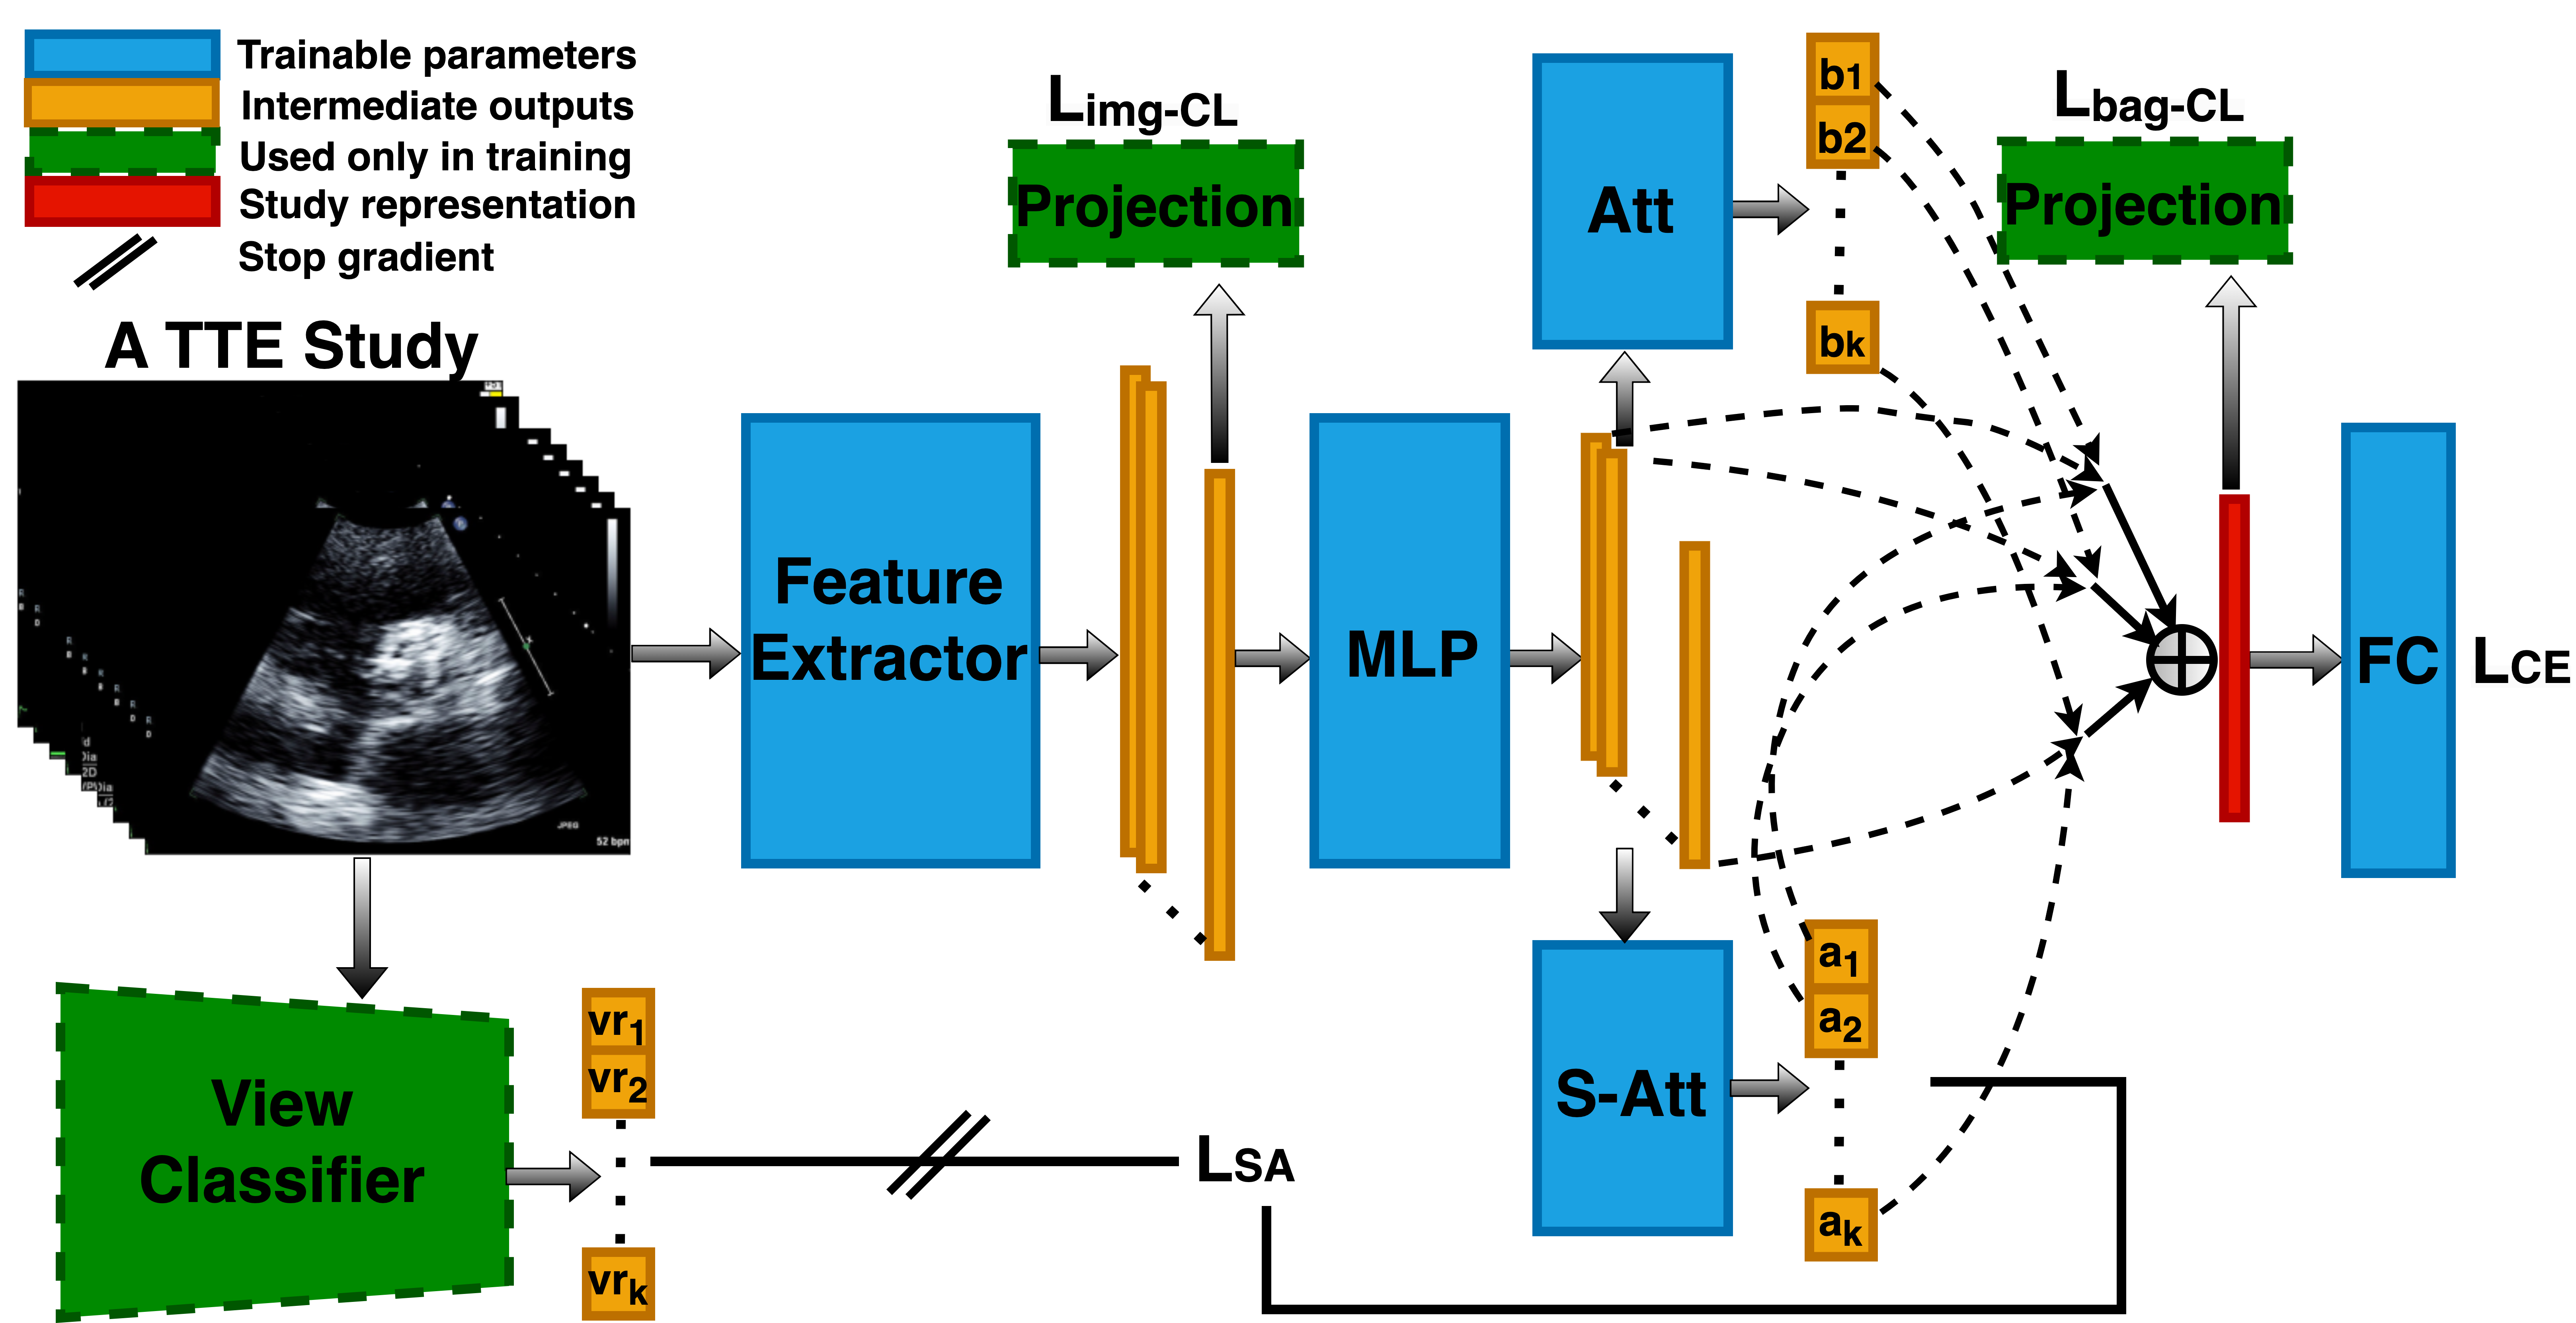
\includegraphics[width=1\textwidth]{figures/SAMIL_diagram_draft1.png}
\caption{\textbf{Overview of proposed method: Supervised Attention Multiple Instance Learning (SAMIL)}.
Given a study or ``bag'' with various images, a feature extractor processes each image individually into an embedding vector. Two attention modules (one supervised by a trained view classifier and one without) produce attention weights for each instance. The final study representation averages the image embeddings weighted by a combination of the two attentions (Eq.~\eqref{eq:patient_embedding_samil}). A fully connected layer then maps the study representation to a diagnosis label. 
\emph{Pretraining:} SAMIL can be pretrained using either bag-level (recommended, Sec.~\ref{sec:methods_CL}) or image-level contrastive learning. In either case, a projection head maps representations to a latent space where the contrastive loss is applied, following \citep{chen2020simple, chen2020improved}. The projection head is discarded after pretraining.
}%endcaption	
\label{fig:workflow_diagram}
\end{figure}
\label{sec:Methods}
\subsection{Problem Formulation}
\label{sec:methods_formulation}

Let $D=\{(X_1, Y_1), \ldots, (X_N, Y_N)\}$ be a training dataset containing $N$ TTE studies. Each study, indexed by $i$, consists of a bag of images $X_i$ and an (optional) diagnostic label $Y_i$.

\textbf{Prediction task.} Given a training set of size $N$, our goal is to build a classifier that can consume a new echo study $X_*$ and assign the appropriate label $Y_*$.

\textbf{Input.}
Each ``bag'' $X_i$ contains $K_i$ distinct images: $\{x_{i1}, x_{i2}, \ldots, x_{iK_i}\}$. These images represent all 2D TTE images gathered during a routine echocardiogram. 
The number of images $K_i$ varies across studies (typical range 27-97).  
Each image $x_{ik}$ is a grayscale image of 112x112 pixels.

\textbf{Output.}
Each study's diagnostic label $Y_i \in \{0, 1, 2\}$ indicates the assessed severity level of aortic stenosis (0 = no AS, 1 =  early AS, 2 = significant AS). These labels are assigned by a cardiologist with specialty training in echocardiography during a routine clinical interpretation of the entire study. Diagnosis labels for individual images are unavailable. 
%Our goal is to build a model that given a new study $S_{new}$ predicts the diagnosis of Aortic Stenosis of this study.   

\textbf{Image preprocessing.}
We used the released dataset directly without additional preprocessing. 
As documented in \citet{huang2022tmed}, the images are extracted from raw DICOM files in the health record by taking the first frame of the corresponding cineloop, removing identifying information, converted to grayscale, padding the shorter axis to a square aspect ratio, and resizing to 112x112. 



\subsection{General MIL architecture}
\label{sec:base_arch}

Following past work on deep neural network approaches to MIL~\citep{ilse2018attention, li2021dual}, a typical architecture has 3 components, as illustrated in Fig.~\ref{fig:diagrams}(d). First, an instance representation layer $f$ transforms each instance into a feature representation. Second, a pooling layer $\sigma$ aggregates across instances to form a bag-level representation in permutation-invariant fashion. Finally, an output layer $g$ 
maps the bag-level representation to a prediction.
%A general procedure for modeling multiple-instance learning problems consists of 3 steps :

%A mapping function $g$ that maps the aggregated feature representation to the bag label. 

We now describe the forward prediction process of one study or ``bag'' $X$ under this 3 component architecture when specialized to our AS severity prediction problem.
Let $X = \{x_1, \ldots, x_K\}$ be the input bag of K instances, with individual instances indexed by integer $k$.
(We use $X$ interchangably with $X_i$ here, dropping the study-specific index $i$ to reduce notational clutter.)

% Our work is built most directly upon ABMIL~\citep{ilse2018attention}, so when needed, we instantiate ABMIL-specific versions of $f$ and $\sigma$.
% For example, Set Transformer \citep{lee2019set} uses an attention mechanism in both $f$ and $\sigma$. ABMIL is simpler, with attention only used in pooling.

 %Our method builds upon ABMIL~\citep{ilse2018attention}, so when needed we instantiate 
%Our method builds up
%ABMIL \citep{ilse2018attention} uses an attention mechanism in pooling function $\sigma$. Set Transformer \citep{lee2019set} uses the attention mechanism in both $f$ and $\sigma$. 

\paragraph{Instance representation layer $f$.} 
Let $f$ be a row-wise feedforward layer that processes each instance $x_k \in \mathcal{X}$ independently and identically, producing an instance-specific embedding $h_k=f(x_k)$, where $h_k \in \mathbb{R}^{M}$. Concretely, we use a stack of convolution layers and a MLP layer to extract and project the instance's feature representation to low-dimensional embedding. More details in App.~\ref{app:Architecture}.
%producing a bag of embeddings
%$H = \{h_1, \ldots, h_K\}$ \in \mathbb{R}^{L \times 1}$. 

\paragraph{Pooling layer $\sigma$.}
ABMIL uses an attention-based pooling method which produces a bag-level representation $z \in \mathbb{R}^{M}$ via an attention-weighted average of the $K$ instance embeddings $\{h_1, \ldots h_K\}$:
\begin{equation}
    \label{eq:patient_embedding_abmil}
    z = \sum_{k=1}^K a_k h_k, \quad 
    a_k = \frac{\exp(w^\top \tanh(U h_k))}{\sum_{j=1}^K \exp(w^\top \tanh(U h_j))},
\end{equation} 

where vector $w \in \mathbb{R}^{L}$ and matrix $U \in \mathbb{R}^{L \times M}$ are trainable parameters of layer $\sigma$. Alternative gated attention modules are also possible, but they tend to yield only marginal gains in classification performance.

\paragraph{Output layer $g$.} Given a bag-level feature vector $z = \sigma(f(X))$, the output layer performs probabilistic classification for the 3 levels of AS severity (0=none, 1=early, 2=significant) via a standard linear-softmax transformation of $z$:
\begin{align}
    p( Y = r | X) = g(z)_r ~\text{for}~ r \in \{0,1,2\}, \qquad g(z) = 
    \left[
    \frac{\exp( \eta_0^{\top} z)}{S(\eta,z)}, \frac{\exp( \eta_1^{\top} z)}{S(\eta,z)}, \frac{\exp( \eta_2^{\top} z)}{S(\eta,z)}
    \right].
\end{align}
Here, $\eta_0, \eta_1, \eta_2$ represent weights for each of the 3 severity levels of AS, and denominator $S = \sum_{r=0}^2 \exp( \eta_r^{\top} z)$ ensures the probabilities sum to one. We do include an intercept term for each class, but omit from notation for clarity.

\paragraph{Training.}
This 3-component deep MIL architecture has parameters $\eta$ for the output layer as well as $\theta$ for the pooling and representation layers ($\theta$ includes $w, U$ from Eq.~\eqref{eq:patient_embedding_abmil}).
We train these parameters by minimizing the cross-entropy loss between each study's observed AS diagnosis $Y$ and the MIL-predicted probabilities given each bag of images $X$ 
\begin{align}
    \theta^*, \eta^* = \arg\!\min_{\theta, \eta} \sum_{X, Y \in \mathcal{D}} \mathcal{L}_{\text{CE}}\left( Y, g_{\eta}( \sigma_{\theta}( f_{\theta}(X) ) \right) 
\end{align}
In practice, weight decay is often used to regularize the model and improve generalization.
% Subscripts here remind us which layers depend on which parameters. In practical, additional regularization such as a weight decay loss may be needed to improve generalization.

% {@MCH I found prior works ususally don't include the WD term when talking about loss function. Shall we follow this convention, so that the notation is cleaner here, also when writing the total loss in Sec 4.5}


% \todo{with standard weight decay}.

% \begin{align}
%     \theta^*, \eta^* = \arg\!\min_{\theta, \eta} ~\sum_{i=1}^N \mathcal{L}_{\text{CE}}\left( Y_i, g_{\eta}( \sigma_{\theta}( f_{\theta}(X_i) ) \right) + \lambda \theta^T \theta + \lambda \eta^T \eta
% \end{align}

% {@MCH I found prior works ususally don't include the WD term when talking about loss function. Shall we follow this convention, so that the notation is cleaner here, also when writing the total loss in Sec 4.5}

\subsection{Contribution 1: Attention supervised by a view classifier}
\label{sec:methods_SA}

We find the attention-based architecture described above yields unsatisfactory performance in our diagnostic task (see table~\ref{tab:TMED2_BACC}). Furthermore, the learned attention values used in Eq.~\eqref{eq:patient_embedding_abmil} do not pass a clinical sanity check: attention should be paid only to PLAX and PSAX AoV view types, as only these show the aortic valve (see fig~\ref{fig:Attention_View_Alignment}).

This last observation suggests a path forward: supervising the attention mechanism. Suppose we have access to a trustworthy \emph{view-type-relevance} classifier $v : \mathcal{X} \rightarrow [0.0,1.0]$, which maps an image to the probability that it shows a relevant view depicting the aortic valve (either a PLAX or PSAX AoV view), rather than another view type (such as A2C, A4C, A5C, etc.).
This classifier could be used to guide the attention to focus on relevant images.
Directly classifying the view-type of a 2D TTE image has been demonstrated with high accuracy by several research groups ~\citep{madani2018fast, zhang2018fully, long2018identification, huang2021new}. 

\paragraph{Supervised attention.}
To implement this idea, we introduce a new loss term, which we call supervised attention (SA), that directly steers the attention weights $A = \{a_1, \ldots a_K\}$ produced by Eq.~\eqref{eq:patient_embedding_abmil} to match normalized relevance scores $R = \{r_1, \ldots r_K\}$ from a view-relevance classifier $v$: 
\begin{equation}
    \label{eq:L_SA}
    \mathcal{L}_{SA}(w, U) = \text{KL}(R || A) = \sum_{k=1}^K r_k \log \frac{r_k}{a_k}, \qquad  r_k = \frac{\exp(v(x_k)/\tau_{v})}{\sum_{k=1}^K \exp( v(x_k) / \tau_{v} ) } 
\end{equation}
%\mch{@HZ, please confirm direction of KL is correct. KL is not symmetric. I would have thought we should do $KL(R || A)$.}

Here, $\text{KL}$ means the KL-divergence between two discrete distributions over the same $K$ categories, and $R \in \Delta^K$ is a non-negative vector that sums to one obtained via a softmax transform of the view relevance probabilities with temperature scaling $\tau_{v} > 0$. We define view relevance probability as the sum of probability that the image is PLAX or PSAX. 

%$KL$ is the KL-divergence. $VR = {vr_1, \ldots, vr_K}$ is a bag of predicted view relevance where $vr_i = p(PLAX|x_i; \theta) + p(PSAX|x_i; \theta)$ and $\theta$ is a pretrained view classifier.
%\begin{equation}
%\phi(vr_i) = \frac{\exp(vr_i/\tau)}{\sum_{i=K}^P \exp(vr_i/\tau)}
%\end{equation} 
%normalize the vector $VR$ to a valid distribution with temperature scaling $\tau$. 

This supervision ensures the MIL diagnostic model attends to instances that are clinically plausible for the disease in question. That is, attention to PLAX or PSAX views that show the aortic valve is encouraged, and attention to irrelevant view types like A4C or A2C is discouraged. 
We emphasize that our approach is classifier-guided because reliable human-annotated labels are not always available. Only 40\% percent of images in TMED-2 training set have view labels. If expert-derived labels were more readily available, we could have supervised directly on those. Using classifier-provided probabilistic labels $R$ allows us to train easily on ``as-is'' data without expensive annotation effort.

Our supervised attention module can be seen as an example of \emph{knowledge distillation}~\citep{hinton2015distilling}, because the MIL model is ``taught'' to output attentions weight similar to the relevant view predictions from the pretrained view classifier. In a sense, the knowledge from the view classifier is distilled directly into the MIL model. 


% regularization guides the MIL model to attend to where it suppose be attend as if it is a cardiologist (e.g., attend to PLAX or PSAX that show the aortic valve, instead of irrelevant background images or irrelevant views like A4C or A2C etc).

\paragraph{View classifier.}
We trained the view classifier via a recently proposed semi-supervised learning method~\citep{huang2022fix} that is shown to be robust to potential unlabeled set noise. The classifier is trained on images with view labels in the train set and all images in the unlabeled set. The classifier is trained to recognize the view type of an image, classifying it as either PLAX, PSAX or Other. To prevent data leakage, separate view classifiers are independently trained for each data split. More details can be found in App ~\ref{app:ViewClassifier}. 

\paragraph{Flexible attention.}
A potential drawback of enforcing strict alignment between attention weights and predicted view relevance is the reduced 
flexibility. Concretely, among the identified relevant view images in a study, we would like the attention weights to have the freedom to focus on one over the other based on how it contributes to the diagnosis. To achieve this, we further introduce another set of attention weights $\mathrm{B} = \{b_1, \dots, b_K\}$.
%\begin{equation}
%    b_i = \frac{\exp(w_{b}^\top \tanh(U_b h_i))}{\sum_{i=1}^K \exp(w_{b}^\top \tanh(U_b h_i))},
%\end{equation} 
Together, the view-classifier-supervised attention $A$ and the flexible attention $B$ are combined to produce the final study-level represention $z \in \mathbb{R}^{M}$ by a simple construction,
\begin{equation}
\label{eq:patient_embedding_samil}
    z = \sum_{k=1}^K c_k h_k, \quad c_k(A,B) = \frac{a_k b_k}{\sum_{j=1}^K a_j b_j }, 
    \quad b_k = \frac{\exp(w_{b}^\top \tanh(U_b h_k))}{\sum_{j=1}^K \exp(w_{b}^\top \tanh(U_b h_j))}.
\end{equation}
In this way, the ultimate attention $c_k$ paid to an image can span the full range of 0.0 to 1.0 if that image is a relevant view, but is likely to be near 0.0 if the classifier deems that image's view irrelevant.
Note that the trainable parameters that determine $B$ -- $w_b \in \mathbb{R}^{L}$ and matrix $U_b \in \mathbb{R}^{L \times M}$ -- are not guided by view-relevance supervision at all, unlike their counterparts $w, U$ that determine $A$.
%from Eq.~\eqref{eq:patient_embedding_abmil}.

%The final attention weights for our model are based on the view regularized attention weights and the free attention weights 
%\begin{equation}
%    \alpha^f_i = \frac{\alpha_i \cdot \beta_i }{\sum_{i=1}^K %\alpha_i \cdot \beta_i} 
%\end{equation}
%And the final representation of the study is 


%move to Related work section
% \paragraph{Related work.}
% C2C~\citep{sharma2021cluster} also use KL-divergence to guide the attention weights, but different from ours the method is proposed for WSI classification. Further, the KL-divergence is measured between the attention weights against a predefined distribution (uniform distribution) with the purpose of minimize intra-cluster variance for patches coming from the same cluster. 


\subsection{Contribution \#2: Contrastive learning of entire study representations}
\label{sec:methods_CL}

Self-supervised learning (SSL) is an effective way to pre-train models that can be later fine-tuned to downstream tasks. 
Most previous methods \citep{holste2022self, holste2022automated, liu2022multiple, lu2019semi, li2021dual, saillard2021self, dehaene2020self, rymarczyk2023protomil}  applying SSL to MIL tasks focus on pretraining the instance-level feature extractor $f$  (or part of $f$) aiming to learn better instance-level feature representation. % processing each image independently.
In contrast, we propose to pretrain the whole MIL network, 
refining the representation vector $z$ encompassing all $K$ images in an echo study. In the vocabulary of MIL, this would also be called the ``bag-level'' representation.
Empirical results in Tab.~\ref{tab:Pretraining strategy ablation} show that our study-level pretraining strategy is better suited for the problem of diagnosing Aortic Stenosis using multi-view ultrasound images, leading to substantial performance gain compared to image-level pretraining.

%\todo{In contrast to most previous methods that pretrain only the feature extractor of the MIL model using each \textbf{image} independently, we propose to pretrain on the whole MIL network with each \textbf{study}, empirical results ~\ref{tab:Pretraining strategy ablation} shows that our pretraining strategy is better suited for the problem of diagnosing Aortic Stenosis using multi-view ultrasound images, leading to substantial performance gain compared to common approaches.}

\paragraph{MoCo(v2) for representations of individual images.}
Our pretraining strategy builds upon MoCo ~\citep{he2020momentum,chen2020improved}, a recent self-supervised learning method that yields state-of-the-art representations. 
MoCo trains useful representations via an instance discrimination task~\citep{wu2018unsupervised, ye2019unsupervised, bachman2019learning}. The learned embedding for a training image is encouraged to be similar to embeddings of slight transformations of itself, while being different from the embeddings of other images.

To obtain embeddings that should be similar, %given a training set of $J$ images $x_j \in \mathcal{X}$, 
each image $x_j$ in training goes through different transformations (e.g., random augmentation) to yield two versions of itself: $x'_j$ and $x^+_j$ (denote as the ``query'' and the ``positive key''). These images are then \emph{encoded} into an $L$-dimensional feature space by composing a projection layer $\psi$ (a feed-forward network with $l_2$ normalization) onto the output of the instance-level representation layer $f$.
% : $\phi = \psi \circ f$.

To obtain embeddings that should be \emph{dissimilar} to a given query, MoCo retrieves $P$ previous embeddings from a first-in-first-out queue data structure.
For each new query, these are treated as $P$ ``negative keys''. In practice, this queue is updated throughout training at each new batch: 
the oldest elements are dequeud and all key embeddings from the current batch are enqueued. $P$ is usually set to the size of the queue \citep{he2020momentum}.  
% \todo{(usually nearly the size of the entire dataset)}.
%Let $N^{-}$ denote the number of elements in the queue, following convention in ~, we set $P$ to $N^{-}$. 

%will be sampled to serve as the embeddings of the ``negative key''. This queue contains the embeddings from previous mini-batches, and is updated each iteration by enqueuing the current minibatch's key embeddings and dequeuing its oldest elements. Let $N^{-}$ denote the number of elements in the queue, following convention in ~\citep{he2020momentum}, we set $P$ to $N^{-}$. 

To train the representation layer $\phi$ given a training set of $J$ images $x_j \in \mathcal{X}$, we minimize this InfoNCE loss~\citep{oord2018representation}:
\begin{equation}
    \label{eq:regular InfoNCE}
    \mathcal{L}_{\text{img-CL}}(\phi_q) = \sum_{j=1}^J -\log \frac{\exp(q_j^{\top} k^+_j/t)}{\exp(q_j^{\top} k^+_j/t)+\sum_{p=0}^P \exp(q_j^{\top} k^{-}_{jp}/t)}, 
    ~ 
    \begin{array}{cc}
    q_j = \phi_{q}(x'_j)
    \\
    k^+_j = \phi_{k}(x^+_j)
    %\\
    %k^-_{jp} = \phi_{k}(x_{jp}^{-})
    \end{array}
\end{equation}
\noindent Here, $q_j \in \mathbb{R}^L$ is an embedding of the ``query'' image, $k_j^+ \in \mathbb{R}^L$ is an embedding of the ``positive key'', and $k^-_{j1}, \ldots k^-_{jP} \in \mathbb{R}^L$ are $P$ embeddings of ``negative keys'' retrieved from the queue. Encoder $\phi = \psi \circ f$ composes a projection head $\psi$ with feature layer $f$. Scalar temperature $t > 0$ is a  hyperparameter~\citep{he2020momentum}. 

To improve representation quality, in MoCo queries and keys are encoded by separate networks: a query encoder $\phi_q$ with parameters $\theta_q$ and a key encoder $\phi_k$ with parameters $\theta_k$. 
%MoCo uses a query encoder $\phi_{q}$ with parameters $\theta_q$ and a key encoder $\phi_{k}$ with parameters $\theta_k$ to encode the queries and keys.
The query encoder $\phi_q$ is trained via standard backpropagation to minimize the loss above. The key encoder $\phi_k$ is only updated via momentum-based moving average of the query encoder: $\theta_k = m \theta_k + (1 - m)\theta_q$.
Momentum $m \in [0, 1)$ is often set to a relatively large value such as 0.999 to make the key embeddings more consistent over time: 



%The encoded queries and keys are then further projected by a projection head $\psi$ (a feed-forward network with $l_2$ normalization) to the embedding space where the contrastive loss is applied. After training, the projection head is discarded~\citep{chen2020simple, chen2020improved}.


%an image-level contrastive learning (``img-CL'') model \textbf{using all images independently} operationalized via the InfoNCE loss shown below ~\ref{eq:regular InfoNCE}:

% \begin{equation}
%     \label{eq:regular InfoNCE}
%     \mathcal{L}_{\text{img-CL}}(\theta_q, \theta_k; x_1, \ldots x_J) = \sum_{j=1}^J -\log \frac{\exp( q_j ^{\top} k^+_j /t)}{\sum_{p=0}^P \exp(q_j^{\top} k^{-}_{jp}/t)},
%     \qquad 
%     \begin{array}{cc}
%     q_j &= f_{\theta_q}(x'_j),
%     \\
%     k^+_j &= f_{\theta_k}(x^+_j)
%     \\
%     k^-_{jp} &= f_{\theta_k}( x_{jp}^{-})
%     \end{array}
% \end{equation} 


% \begin{equation}
%     \label{eq:regular InfoNCE}
%     % \mathcal{L}_{\text{img-CL}}(\theta_q, \theta_k; x_1, \ldots x_J) = \sum_{j=1}^J -\log \frac{\exp( f_{proj}(q_j ^{\top}) f_{proj} (k^+_j) /t)}{\sum_{p=0}^P \exp(f_{proj} (q_j^{\top}) f_{proj}(k^{-}_{jp})/t)},
%     \mathcal{L}_{\text{img-CL}}(\theta_q, \theta_k, \theta_p; x_1, \ldots x_J) = \sum_{j=1}^J -\log \frac{\exp(s(q_j, k^+_j)/t)}{\exp(s(q_j, k^+_j)/t+\sum_{p=0}^P \exp(s(q_j, k^{-}_{jp})/t)}, 
%     \quad 
%     \begin{array}{cc}
%     q_j &= f_{\theta_q}(x'_j),
%     \\
%     k^+_j &= f_{\theta_k}(x^+_j)
%     \\
%     k^-_{jp} &= f_{\theta_k}( x_{jp}^{-})
%     \\
%     s(a, b) &= \frac{f_{p}(a)^{\top}f_{p}(b)}{ \lVert (f_{p}(a))^ \rVert \lVert f_{p}(b) \rVert}
%     \end{array}
% \end{equation} 

%(a different augmented version of the ``query'' image)



% MoCo uses a dictionary lookup metaphor to understand obtaining the ``key'' embeddings $k^+$ and $k^-$ given a specific query image.
% During training, each image $x_j$ in a batch goes through prescribed transformations (e.g., random augmentation) to yield two versions, $x'_j$ and $x^+_j$. Let's denote $x'_j$ as the ``query'', then $x^+_j$ is the ``positive key''.  The ``query'' will be encoded by the query encoder to obtain encoded ``query'' $q_j = f_{\theta_q}(x'_j)$. The ``positive key'' will be encoded by the key encoder to obtain the encoded ``positive key'' $k^+_j = f_{\theta_k}(x^+_j)$. $P$ ``negative keys'' will be sampled from a first-in-first-out queue data structure that contains the encoded ``keys'' from previous mini-batches. The queue is updated each iteration by enqueuing the current minibatch's key vectors and dequeuing its oldest keys. Let $N^{-}$ denote the number of elements in the queue, following convention in ~\citep{he2020momentum}, we set $P$ to $N^{-}$. $m$ is often set to a relatively large value such as 0.999 to make the encoded keys more consistent over time.

%The two images will then be passed to the query encoder and key encoder respectively to get representation $e_q$ and $e_k$, which form a positive pair. 
% To form negative pairs, MoCo uses a first-in-first-out queue data structure.
% Let $N_{-}$ denote the number of elements in the queue, where each element is the embedding from the key encoders from previous batches. 

%where  $q = f_q(x^q)$ is the feature representation of query image $x^q$ from an encoder network $f_q$. $x^k$ is the positive sample of $x^q$ and likewise, $k = f_k(x^k)$ is the feature representation.

% An important part of MoCo is that the encoding of query images and key images are handled by different weight parameters $\theta_q$ and $\theta_k$ for the same featurization network $f$. The query parameters are trained via standard backpropagation, while the key-embedding parameters are updated given the latest query-embedding parameters with some momentum $m > 0$
% \begin{equation}
% \theta_k = m \theta_k + (1 - m)\theta_q
% \end{equation}
%MoCo uses a query encoder $f_q$ and a key encoder $f_k$, where the query encoder is trained via backpropagation and $f_k$ is updated using $f_q$ with momentum parameter $m$. Let $\theta_k$ and $\theta_q$ be parameters of $f_k$ and $f_q$. $\theta_k$ is updated by:


% \todo{cut this parag?} InfoNCE is one example of a family of so-called \emph{contrastive} losses~\citep{hadsell2006dimensionality}. 
% Comments: other forms of contrastive loss exist, such as 'Unsupervised learning of visual representations using videos', 'Unsupervised feature learning via non-parametric instance discrimination', ' Learning deep representations by mutual information estimation and maximization'

%Intuitively, the instance discrimination task together with the InfoNCE loss pull together positive pairs of images(two transformed versions of the same image) while push away negative pairs of images (an image with all other images). 


%MoCo regards self-supervised learning as a dictionary look-up problem. It achieves representation learning by training the model to output similar representations for the query and its matching keys, and dissimilar representations for the query and other keys. MoCo uses a query encoder $f_q$ and a key encoder $f_k$, where the query encoder is trained via backpropagation and $f_k$ is updated using $f_q$ with momentum parameter $m$. Let $\theta_k$ and $\theta_q$ be parameters of $f_k$ and $f_q$. $\theta_k$ is updated by:
%\begin{equation}
%\theta_k = m\theta_k + (1 - m)\theta_q
%\end{equation}

\paragraph{Adapting MoCo to bag-level representations.}
%\todo{(@MCH we say 'many prior studies', do we need to cite more here?)} 

Most prior studies in the MIL literature, such as  ~\citet{li2021dual},  use an ``off-the-shelf'' version of contrastive learning algorithm (e.g., SimCLR ~\citep{chen2020simple} or MoCo~\citep{he2020momentum,chen2020improved}) to pretrain image-level feature extractor $f$ like we illustrated above.
However, we find that naively applying MoCo in this way does not yield useful results for our AS diagnosis problem.

Reasoning that what ultimately matters is the quality of the study-level representation $z$ produced by our MIL architecture, we adapted MoCo to produce solid representations of entire echocardiogram studies.
Correspondingly, we modified the InfoNCE loss to operate on the bag-level representations $z$. Given a training set of $N$ bags $X_1, \ldots X_N$, our approach to ``bag-level'' contrastive learning tries to pull together positive pairs of \emph{studies} and push away (make dissimilar) negative pairs of studies, via the loss
%~\ref{eq:our InfoNCE}
% \begin{equation}
%     \label{eq:our InfoNCE}
%     \mathcal{L}_{\text{bag-CL}}(\theta_q, \theta_k; X_{1:N}) = \sum_{i=1}^N -\log \frac{\exp(z_i^{\top} z^+_i / t)}{\sum_{p=0}^P \exp(z_i^{\top} z_{ip}^-/t)}, 
%     \quad
%     \begin{array}{cc}
%          z_i &= \sigma_{\theta_q}(f_{\theta_q}(X'_i)),
%          \\
%          z^+_i &= \sigma_{\theta_k}(f_{\theta_k}(X^{+}_i)),
%          \\
%          z^{-}_{ip} &= \sigma_{\theta_k}(f_{\theta_k}(X^{-}_{ip})).
%     \end{array}
% \end{equation} 

% \begin{equation}
%     \label{eq:our InfoNCE}
%     \mathcal{L}_{\text{bag-CL}}(\theta_q, \theta_p; X_{1:N}) = \sum_{i=1}^N -\log \frac{\exp(s(z_i, z^+_i)/ t)}{\exp(s(z_i, z^+_i)/ t) + \sum_{p=0}^P \exp(s(z_i, z^{-}_{ip})/t)}, 
%     \quad
%     \begin{array}{cc}
%          z_i &= \sigma_{\theta_q}(f_{\theta_q}(X'_i)),
%          \\
%          z^+_i &= \sigma_{\theta_k}(f_{\theta_k}(X^{+}_i)),
%          \\
%          z^{-}_{ip} &= \sigma_{\theta_k}(f_{\theta_k}(X^{-}_{ip})).
%          \\
%         s(a, b) &= \frac{f_{p}(a)^{\top}f_{p}(b)}{ \lVert (f_{p}(a))^ \rVert \lVert f_{p}(b) \rVert}
%     \end{array}
% \end{equation} 

\begin{equation}
    \label{eq:our InfoNCE}
    \mathcal{L}_{\text{bag-CL}}(\phi_q; X_{1:N}) = \sum_{i=1}^N -\log \frac{\exp(\tilde{z_i}^{\top} \tilde{z_i}^{+}/t)}{\exp(\tilde{z_i}^{\top} \tilde{z}_i^{+}/t) + \sum_{p=0}^P \exp(\tilde{z_i}^{\top} \tilde{z}_{ip}^{-})/t)}, 
    ~
    \begin{array}{cc}
         \tilde{z_i} = \phi_q(X'_i),
         \\
         \tilde{z_i}^{+} = \phi_k(X^{+}_i),
    \end{array}
\end{equation} 

% \begin{equation}
%     \label{eq:our InfoNCE}
%     \mathcal{L}_{\text{bag-CL}}(\theta_q, \theta_p; X_{1:N}) = \sum_{i=1}^N -\log \frac{\exp(z_i^{\top} z^+_i/ t)}{\exp(z_i^{\top} z^+_i/ t) + \sum_{p=0}^P \exp(z_i^{\top} z^{-}_{ip}/t)}, 
%     \quad
%     \begin{array}{cc}
%          z_i &= \sigma_{_q}(f_{_q}(X'_i)),
%          \\
%          z^+_i &= \sigma_{k}(f_{k}(X^{+}_i)),
%          \\
%          z^{-}_{ip} &= \sigma_{\theta_k}(f_{\theta_k}(X^{-}_{ip})).
%          \\
%         s(a, b) &= \frac{f_{p}(a)^{\top}f_{p}(b)}{ \lVert (f_{p}(a))^ \rVert \lVert f_{p}(b) \rVert}
%     \end{array}
% \end{equation} 

Here, $\phi = \psi \circ \sigma \circ f$. $f$ and $\psi$ are the same feature extractor and projection head as in image-level case. However, a pooling layer $\sigma$ is used and the input is now \textbf{all the images in a study}. $\tilde{z}=\psi(z)$ is the projection of $z$, $z_{i} = \sigma_q(f_q(X_i'))$ is the bag-level representation of the ``query'' study, and $z_{i}^{+} = \sigma_k(f_k(X_i^{+}))$ is the bag-level representation of the ``positive key'' study.
$X'$ and $X^+$ are obtained from the given study $X$ by applying different random augmentation to each of its images. 
$\tilde{z_{ip}}^{-}$ are again sampled from the queue. The enqueue and dequeue mechanism of the queue and the update rules of $\phi_q$ and $\phi_k$ are the same as the image level case. 

% Here, we use $z$ variables to denote embeddings of entire bags (entire echo studies for our application).
% For simplicity, parameters 
% $\theta_q$ and $\theta_k$ represent \emph{all} parameters needed, unifying the set of parameters required by pooling $\sigma$ and featurization $f$ functions.




%$X$ in eq ~\ref{eq:our InfoNCE} is the whole bag of images from a study instead of an individual image used in eq~\ref{eq:regular InfoNCE}. $z=\sigma(f(X))$ is the patient level representation obtained in eq ~\ref{eq:patient_embedding}, and $\sigma$, $f$ are the corresponding pooling function and row-wise feedforward layer in the MIL network. 

\subsection{SAMIL Pipeline}
% \paragraph{self-supervised pretraining.} We pretrain the MIL network using studies in the labeled train set (both the view labeled images and the view unlabeled images in the study are used), as well as the large unlabeled set with our proposed bag-level pretraining strategy (see ~\ref{sec:methods_CL}). The projection head $f_{p}$ is discarded following convention ~\citep{chen2020improved, chen2020simple}.

\paragraph{Self-Supervised Pretraining} 
We pretrain our SAMIL network on TMED-2 data utilizing our proposed bag-level pretraining strategy (Sec.~\ref{sec:methods_CL}).  This method can learn from all available studies, including both the labeled train set as well as the much larger unlabeled set (over 350,000 images).
After pretraining finishes, following convention~\citep{chen2020improved, chen2020simple}, the projection head $\psi_q$ is discarded, and parameters of $\sigma_q$ and $f_q$ are retained to warm-start the supervised fine-tuning. More details in App~\ref{app:SSL_Pretraining}.

% \paragraph{supervised fine-tuning of MIL using diagnosis label}

% We initialize the MIL network with the self-supervised pretrained weights. Next, we fine-tune the MIL network using studies in the labeled train set (both the view labeled images and the view unlabeled images in the study are used), supervised by the diagnosis label of each study, minimizing the loss
% \begin{equation}
%     \mathcal{L} =  \mathcal{L}_{CE} + \lambda \mathcal{L}_{SA}
%     % \mathcal{L}_{SA}(w, U) = \text{KL}(R || A) = \sum_{k=1}^K r_k \log \frac{r_k}{a_k}, \qquad  r_k = \frac{\exp(v(x_k)/\tau_{v})}{\sum_{k=1}^K \exp( v(x_k) / \tau_{v} ) }    
% \end{equation}
% Where $L_{CE}$ is the standard cross-entropy loss and $L_{SA}$ is the supervised attention loss in ~\ref{eq:L_SA}. Overall workflow can be seen in Fig~\ref{fig:workflow_diagram}.

\paragraph{Supervised Fine-Tuning of MIL Using Diagnosis Label}
We initialize our SAMIL network (Fig.~\ref{fig:workflow_diagram}) with the self-supervised pretrained weights, then fine-tune it using studies from TMED2's labeled train set by minimizing the overall loss 
\begin{equation}
\label{eq:total_loss}
\mathcal{L} = \mathcal{L}_{CE} + \lambda_{SA} \mathcal{L}_{SA},
\end{equation}
Here, the primary supervision signal comes from the diagnosis label for each study (via cross entropy loss $\mathcal{L}_{CE}$), while the predicted view probabilities of each image from the view classifier provide additional supervision to the attention module (via supervised attention loss $\mathcal{L}_{SA}$). 
Hyperparameter $\lambda_{SA}$ balances the weights of the two loss terms. 
Each study's bag $X$ contains all available 2D images (regardless of view label availability).


\section{Results} 
\label{sec:Results}
\input{results.tex}
 
\section{Discussion} 
\label{sec:Discussion}
We have developed an approach to deep multiple instance learning for diagnosing a common heart valve disease (aortic stenosis) from the dozens of images collected in a routine echocardiogram. In our evaluations on the open-access TMED-2 dataset, we find our approach reaches better classifier accuracy than several alternatives, including two recent methods dedicated to AS screening. 
We suspect that gains come from two sources. First, our method's ability to use both PLAX and PSAX images, not just PLAX. Second, our method's flexible attention that does not weight each relevant view equally. Both prior efforts on AS studied here, Filter-then-Average and Weighted Average by View Relevance, essentially treat each high-confidence PLAX or PSAX image equally in diagnosis. Instead, we emphasize that our method can learn a study-specific subset of PLAX or PSAX to attend to, based on image quality, anatomic visibility, or other factors.

\paragraph{Limitations in diagnostic potential.}
Human experts assess AS using several additional factors not available to our method. These include patient demographics, clinical variables, and (most importantly) other imaging technologies such as doppler echocardiography as well as high-resolution cineloop videos from 2D TTE (not just lower-resolution single frame images used here). 
We suspect adapting our MIL architecture to these modalities would provide exciting further gains.

\paragraph{Limitations in evaluation.}
As of this writing, TMED-2 is the only open-access dataset of echos known to us with diagnostic labels for AS or other valve disease.
However, it is limited in size and in covered demographics due to drawing from just one hospital site.
Further assessment is needed to understand how our proposed method generalizes, especially to populations underrepresented at the Boston-based hospital where this data was collected.


\paragraph{Advantages.}
Our SAMIL approach is designed to perform automatic screening of an echo study without requiring a first-stage manual or automatic prefiltering to relevant view types.
Even though prefiltering may sound simpler than MIL, we show our approach works better, likely due to its flexible attention mechanism. 
We can further leverage large unlabeled data collections for pretraining effective representations.

Our MIL approach could easily be applied to other structural heart diseases including cardiomyopathies and mitral and tricuspid disease if suitable labels were available for some studies. Additionally, multi-view image diagnostic problems are also abundant in fetal ultrasound, lung ultrasound, and head CT applications, so we expect translation of our insights to these other domains will bear fruit. Both key innovations -- supervised attention to steer toward clinically-relevant views for the diagnostic task and study-level representation learning -- are applicable to many other prediction tasks.
Ultimately, we hope our study plays a part in transforming early screening for AS and other burdensome diseases to be more reproducible, effective, portable, and actionable. 



% ACKNOWLEDGEMENTS ONLY GO IN THE CAMERA-READY, NOT THE SUBMISSION
\acks{
We acknowledge financial support from the Pilot Studies Program at the Tufts Clinical and Translational Science Institute (Tufts CTSI NIH CTSA UL1TR002544). We are grateful for computing infrastructure support from the Tufts High-performance Computing cluster, partially funded by the National Science Foundation under grant OAC CC* 2018149.
Author B. W. was supported in part by K23AG055667 (NIH-NIA).
}

\begin{small}
\bibliography{refs_manual.bib}    
\end{small}

\appendix

%% Config Table-of-Contents to track the sections of the appendix
\startcontents[sections]

\counterwithin{table}{section}
\setcounter{table}{0}
\counterwithin{figure}{section}
\setcounter{figure}{0}
%\counterwithin{algorithm}{section}
%\setcounter{algorithm}{0}

%% Use ONE counter for all figs and tables to give unique identifiers in supplement
\makeatletter 
\let\c@table\c@figure
\let\c@lstlisting\c@figure
\let\c@algorithm\c@figure
\makeatother

% Print Table of Contents
\subsection*{Appendix Contents}
\printcontents[sections]{l}{1}{\setcounter{tocdepth}{2}}

\section{Further Results}
\subsection{Confusion matrix}
\newcommand{\BW}{0.29}
\setlength{\tabcolsep}{0.05cm}
% \begin{figure}[!h]
\begin{figure}[H]
\begin{tabular}{r c c c }
    & Split 1 & Split 2 & Split 3
    \\
    {\rotatebox{90}{~~~~~W. Avg. by View Rel.}}
    & 
    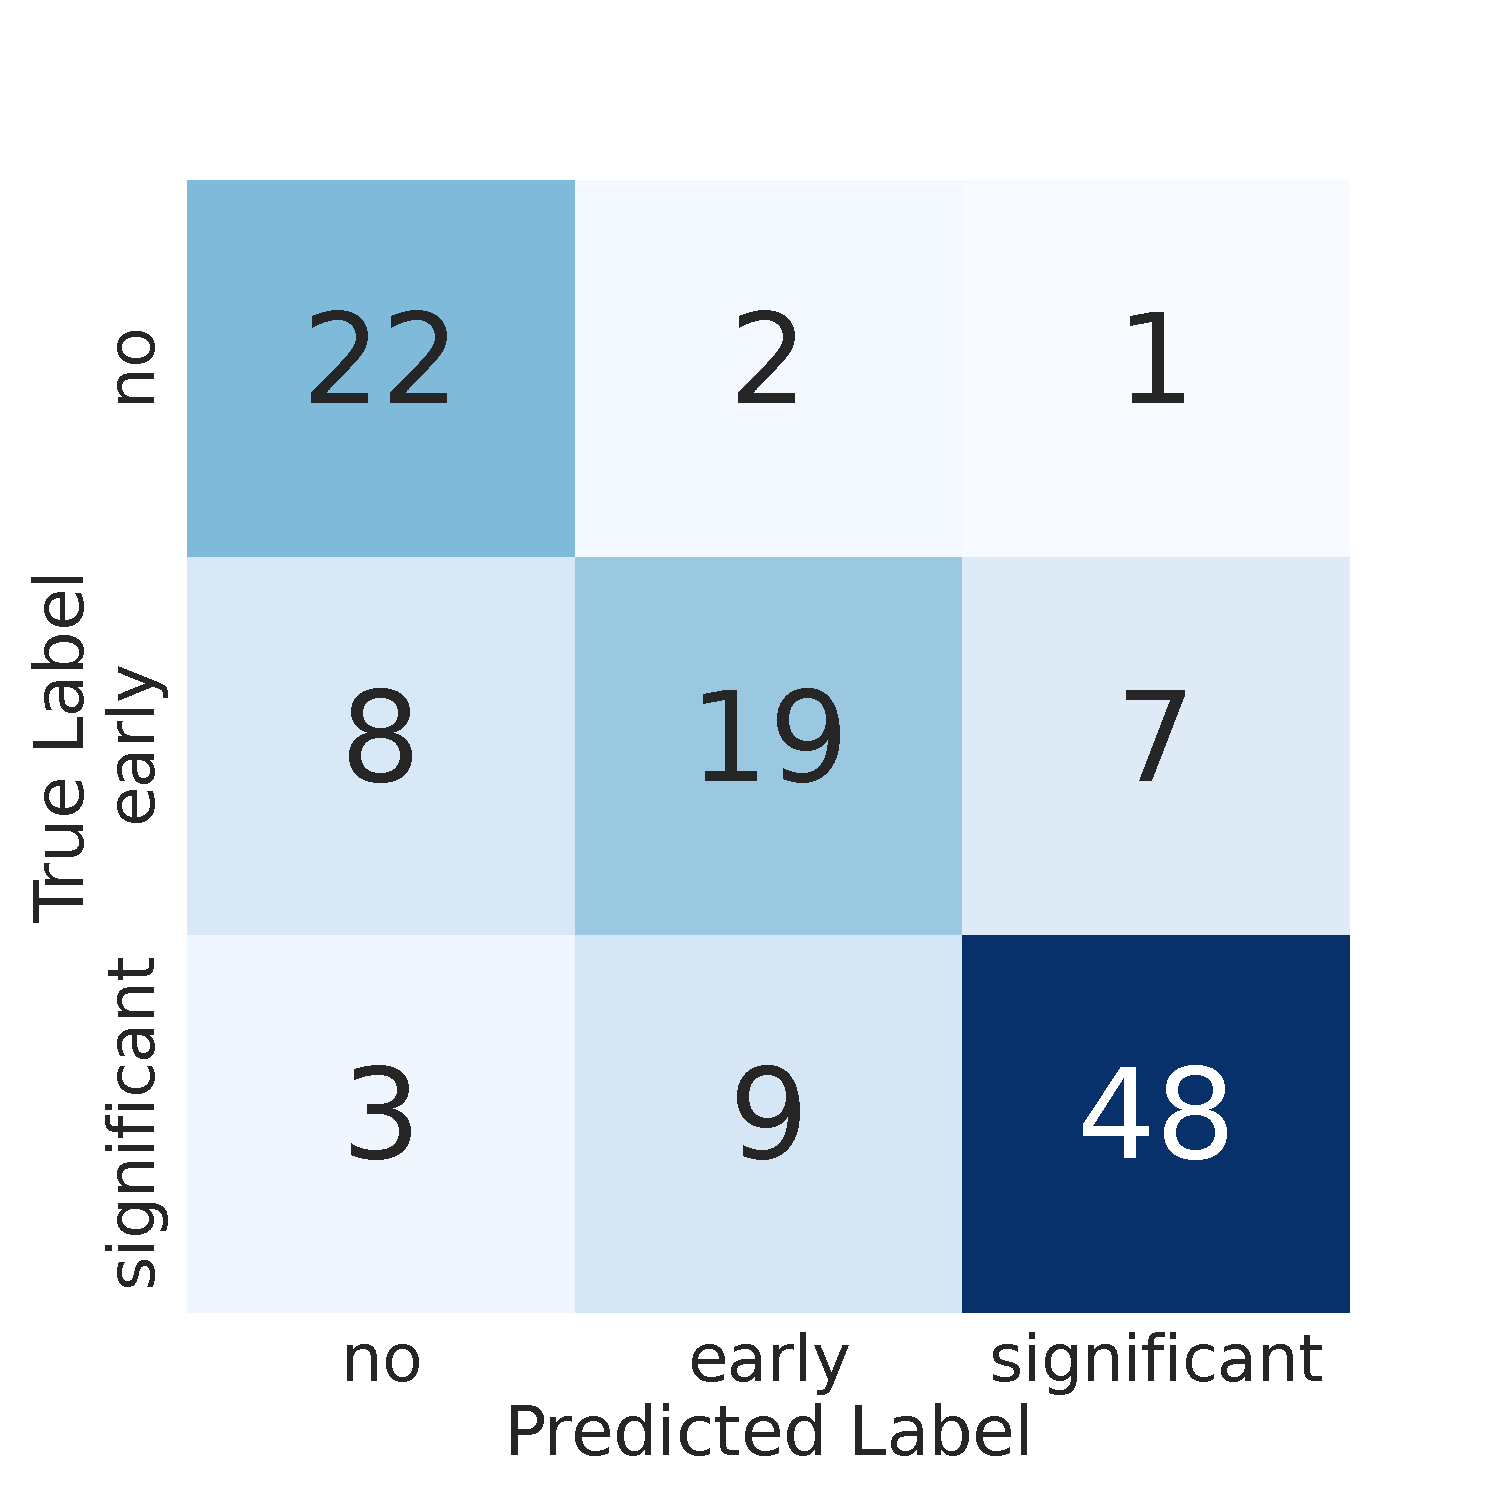
\includegraphics[width=\BW\textwidth]{figures/confusion_matrix/cropped_seed0/JASE.pdf}
    &
    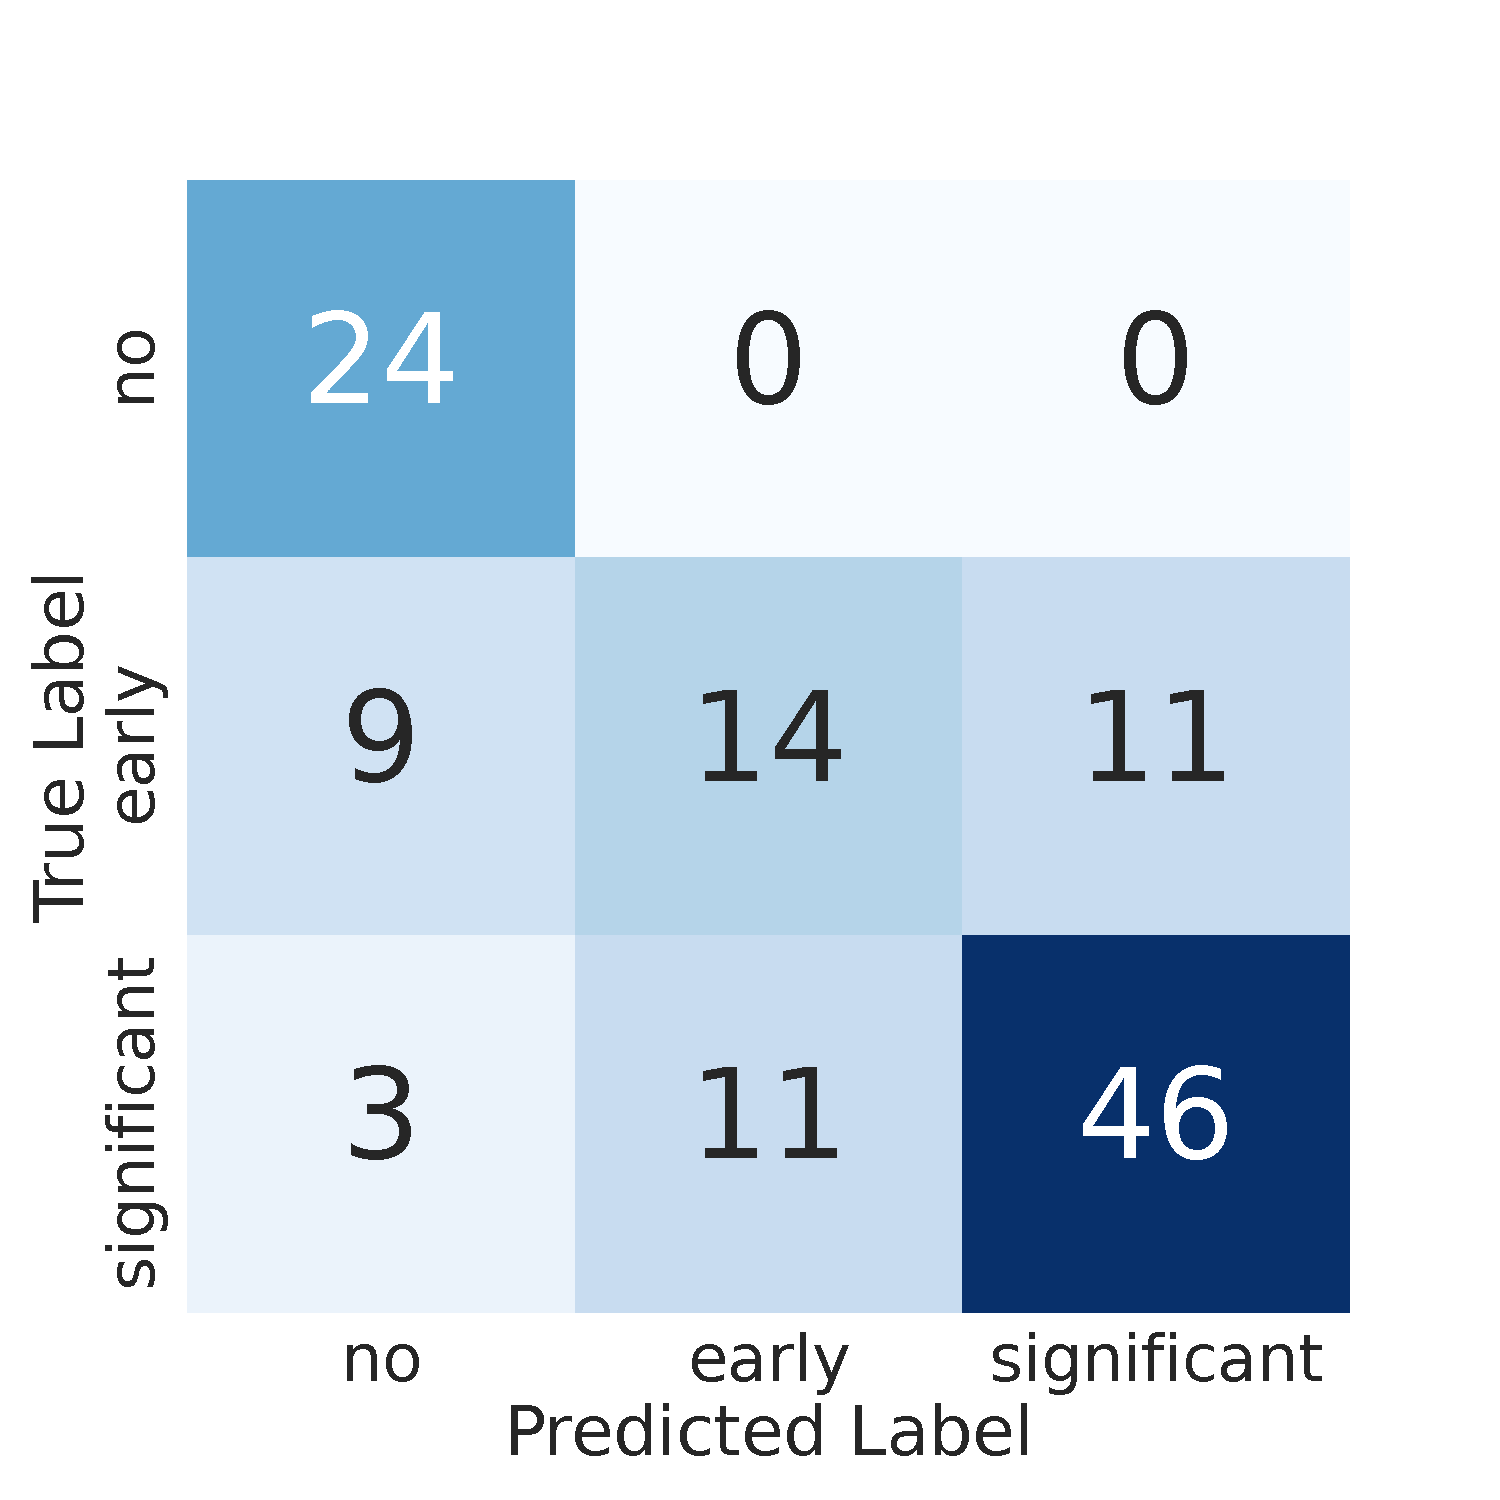
\includegraphics[width=\BW\textwidth]{figures/confusion_matrix/cropped_seed1/JASE.pdf}
    &
    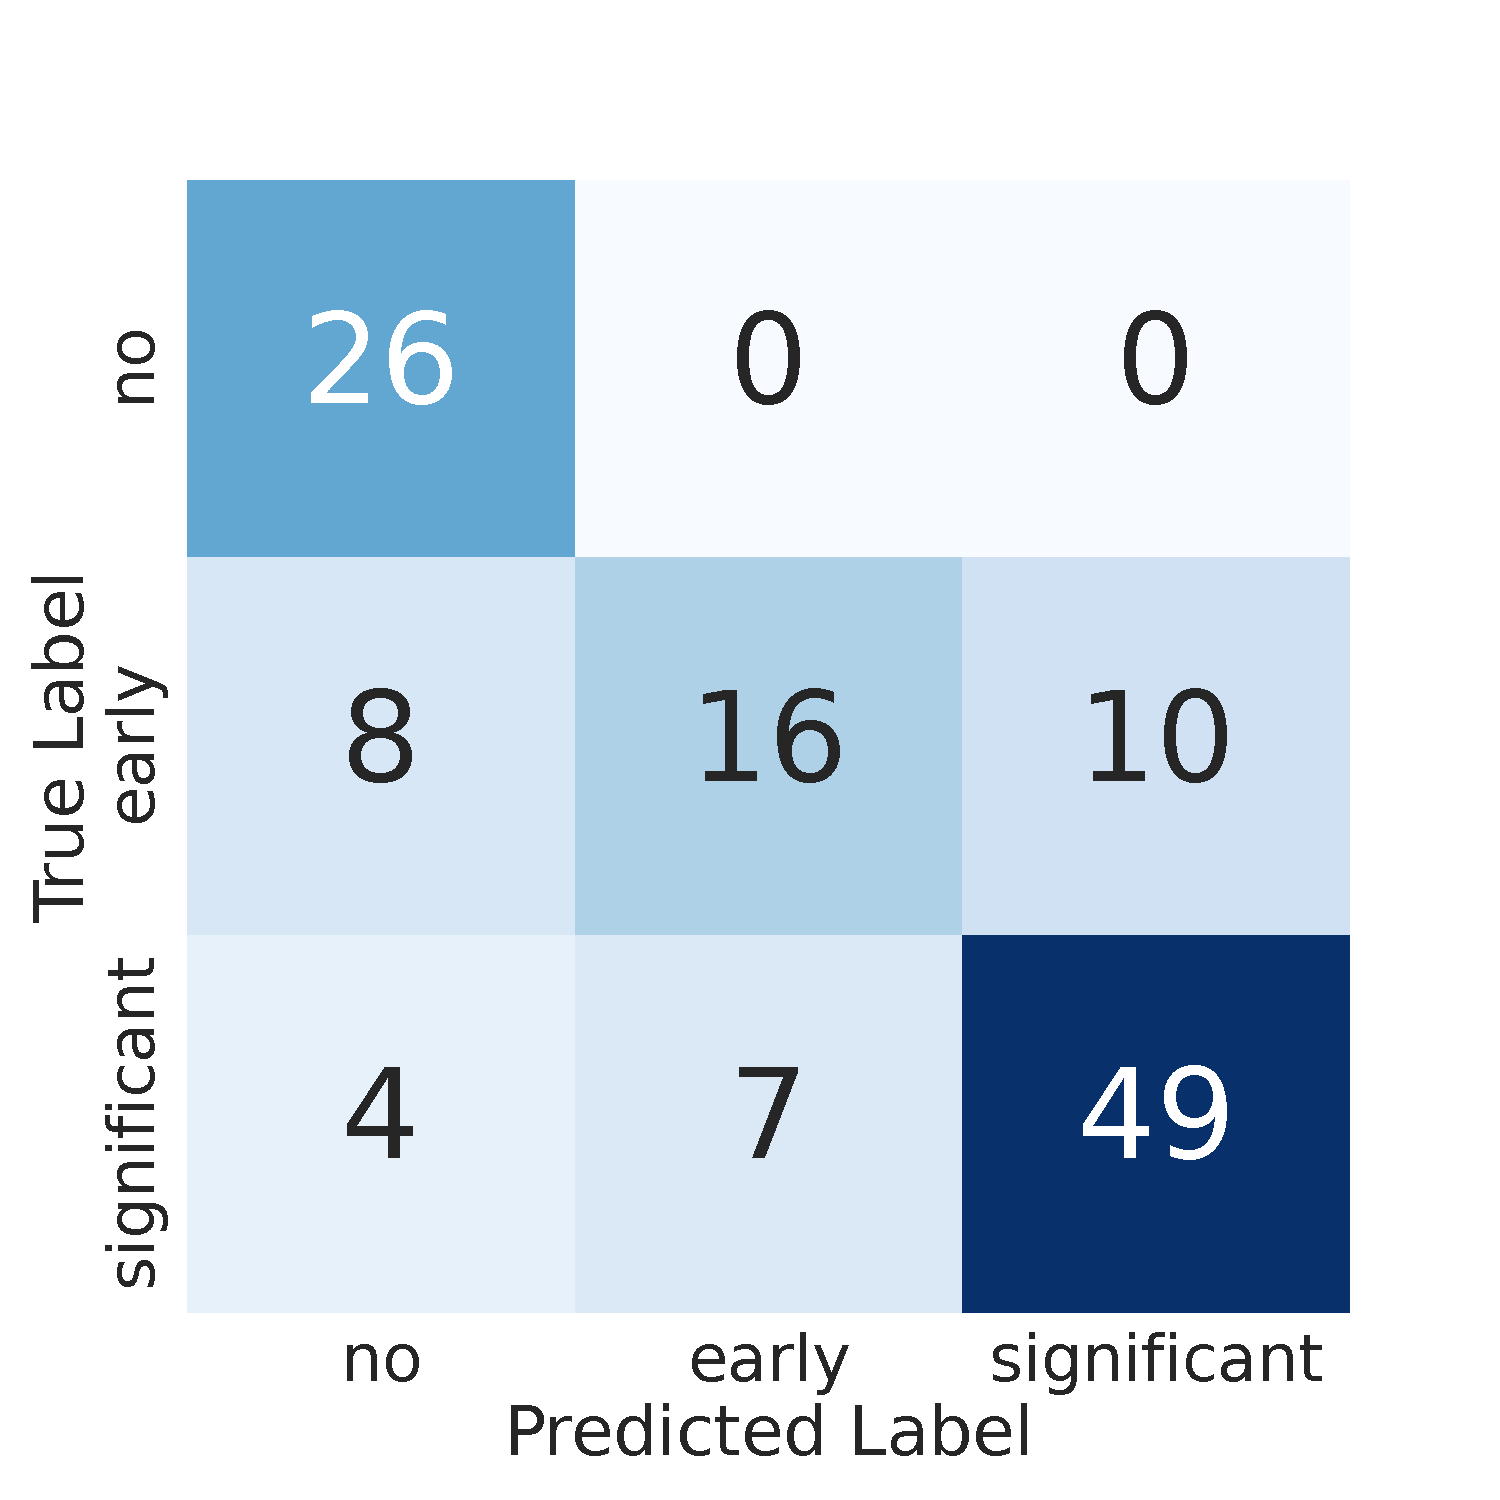
\includegraphics[width=\BW\textwidth]{figures/confusion_matrix/cropped_seed2/JASE.pdf}
    \\
    {\rotatebox{90}{~~~~~~~~~~~~ABMIL}}
    & 
    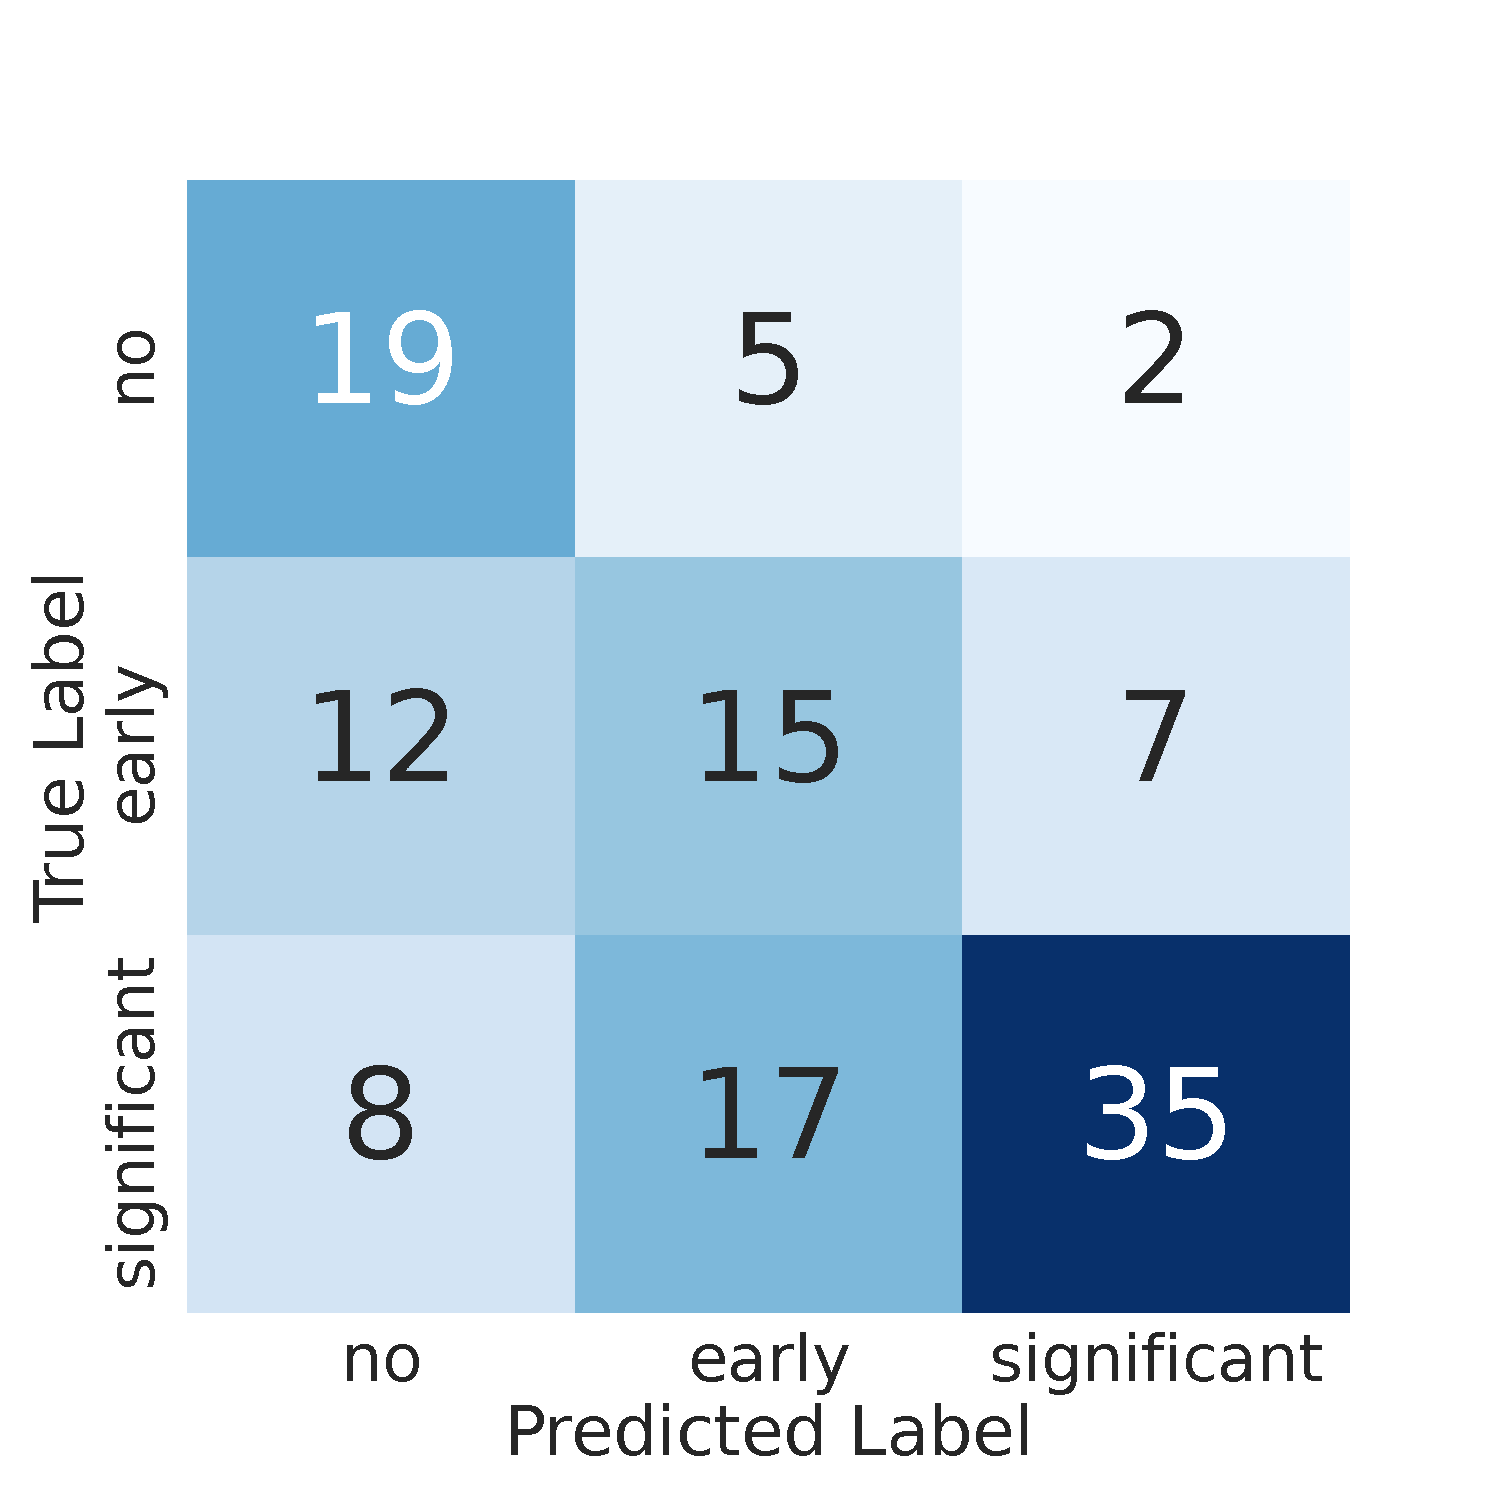
\includegraphics[width=\BW\textwidth]{figures/confusion_matrix/cropped_seed0/OffTheShelfABMIL.pdf}
    &
    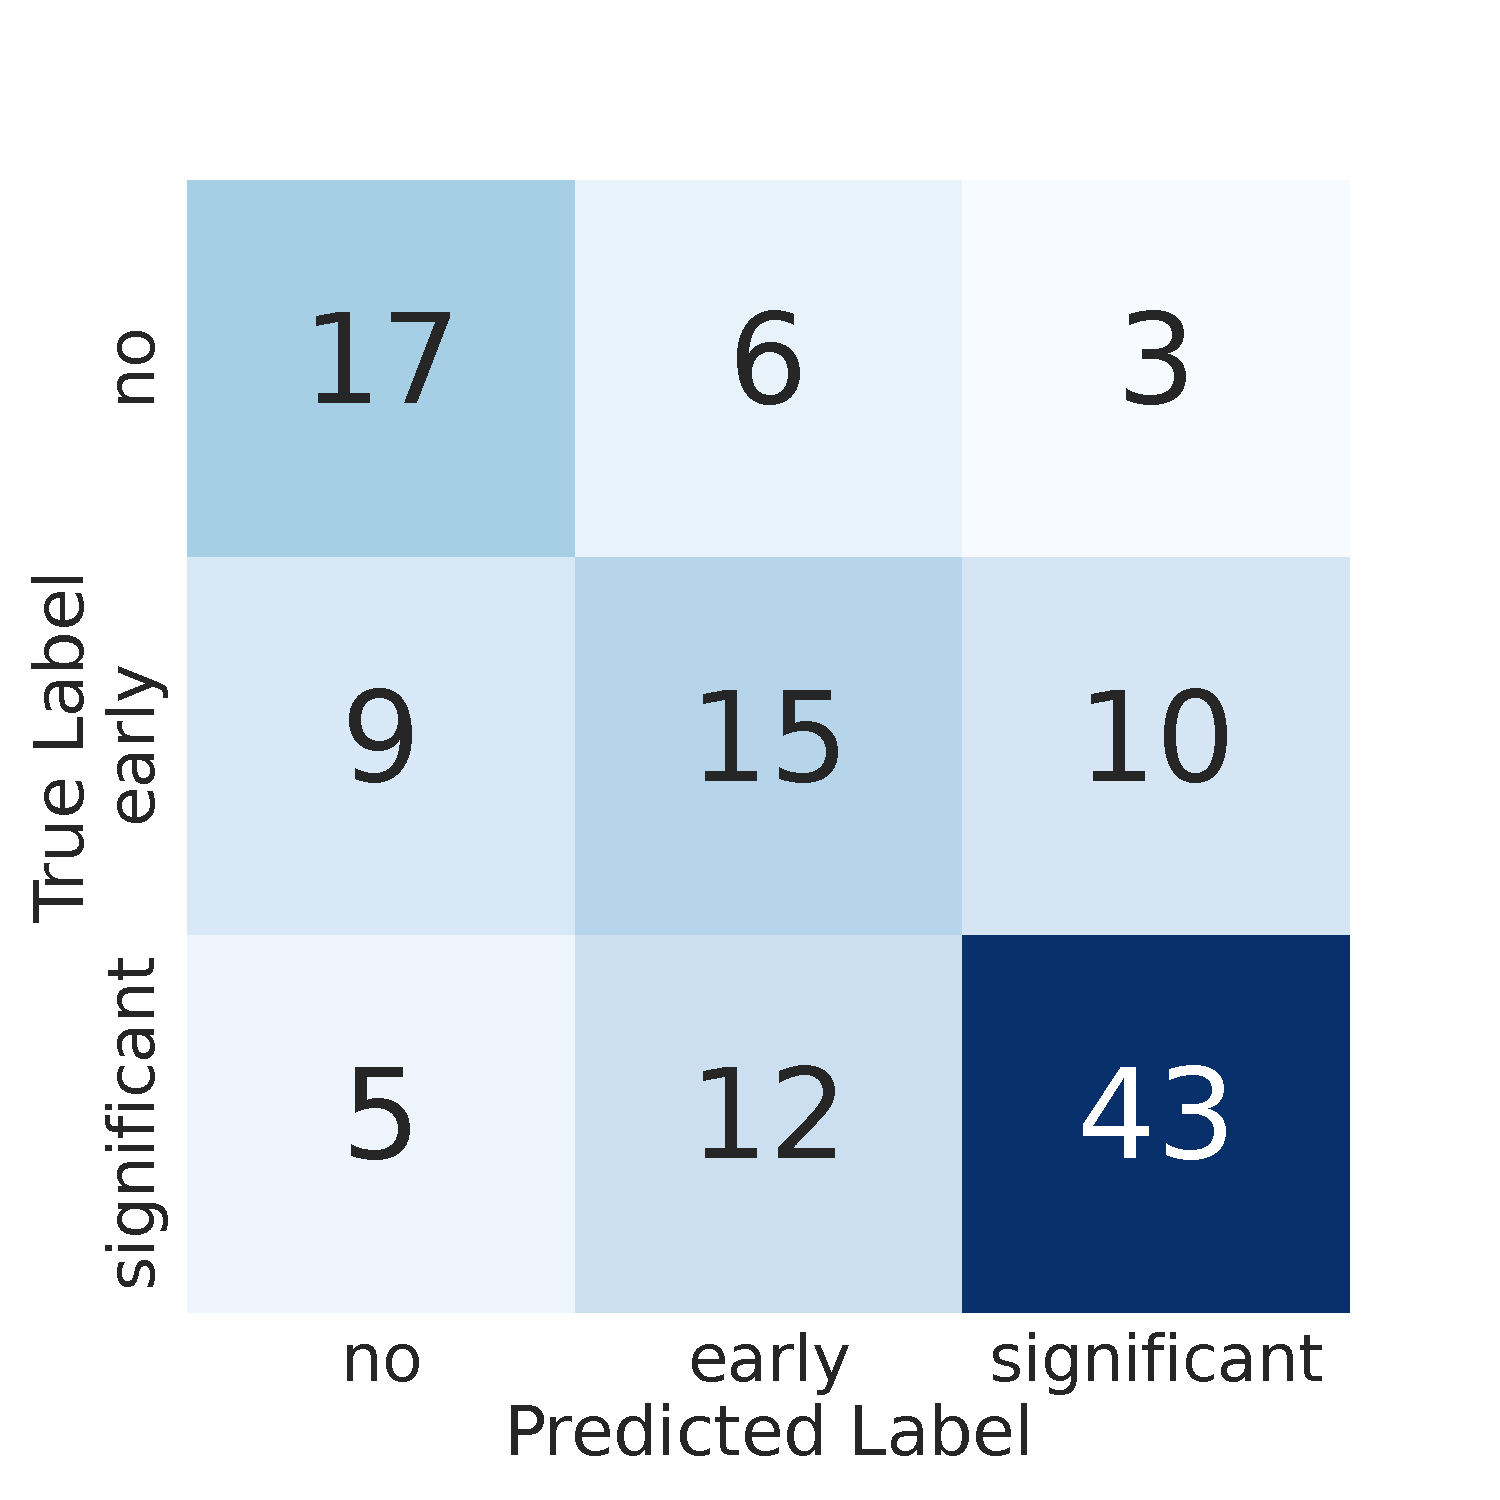
\includegraphics[width=\BW\textwidth]{figures/confusion_matrix/cropped_seed1/OffTheShelfABMIL.pdf}
    &
    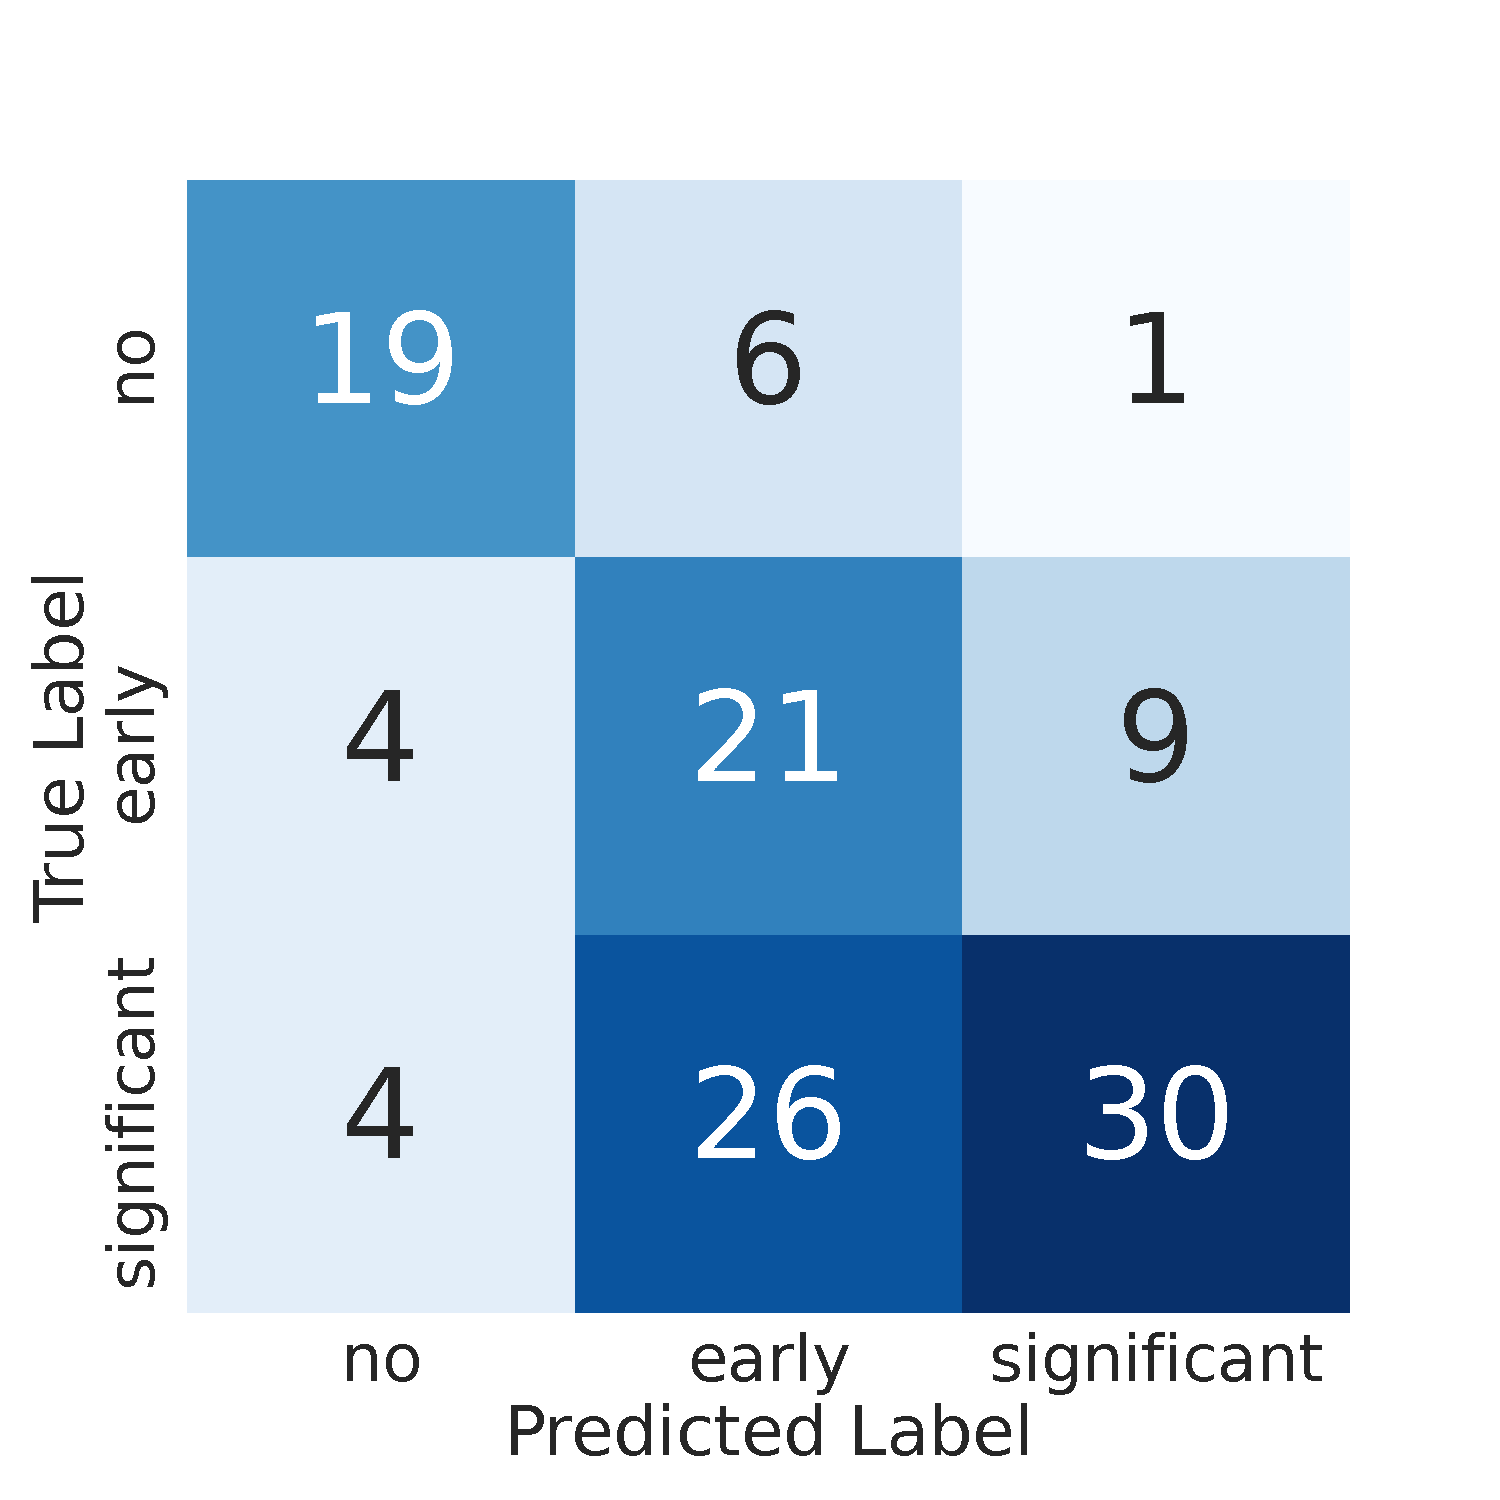
\includegraphics[width=\BW\textwidth]{figures/confusion_matrix/cropped_seed2/OffTheShelfABMIL.pdf}
    \\
    {\rotatebox{90}{~~~~~~~~~~~~DSMIL}}
    & 
    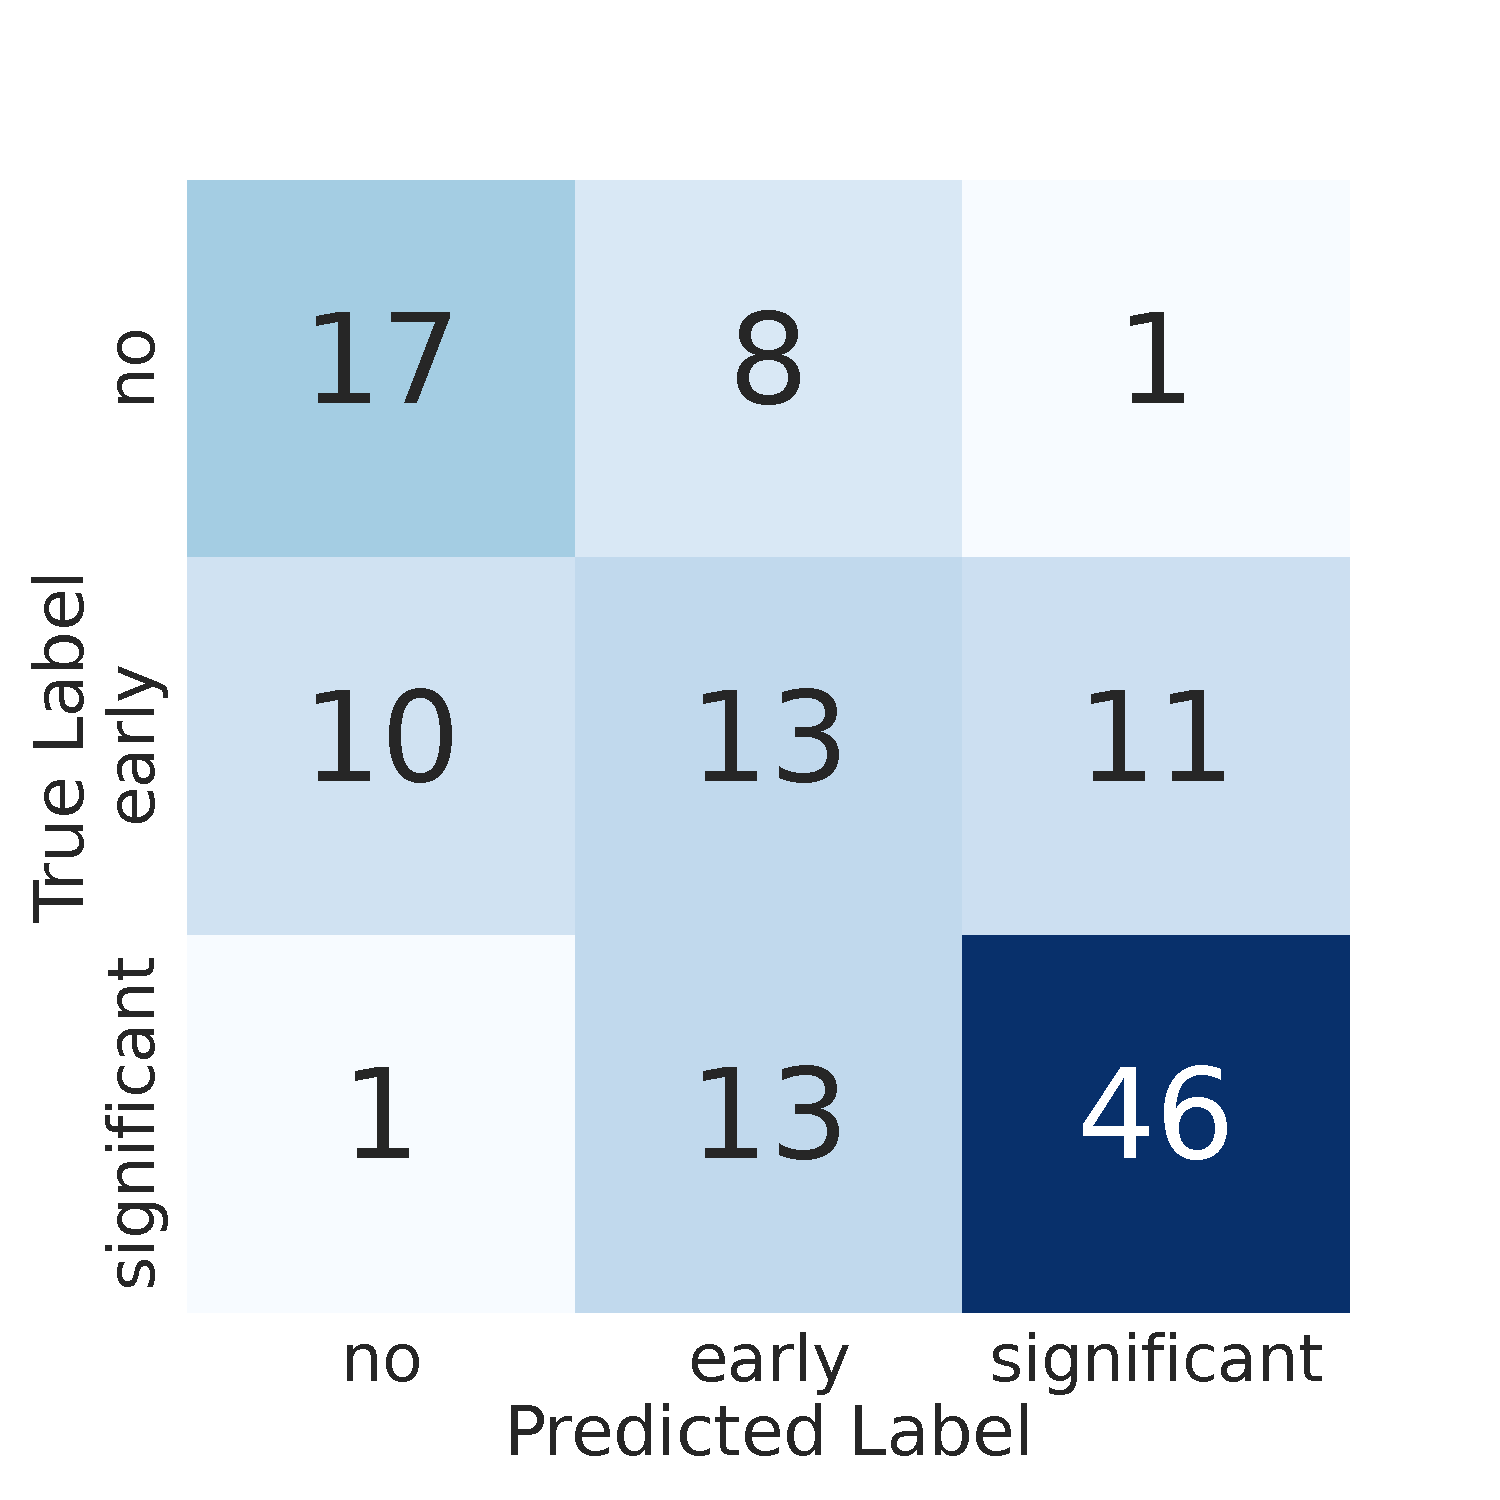
\includegraphics[width=\BW\textwidth]{figures/confusion_matrix/cropped_seed0/OffTheShelfDSMIL_updatedseed0.pdf}
    &
    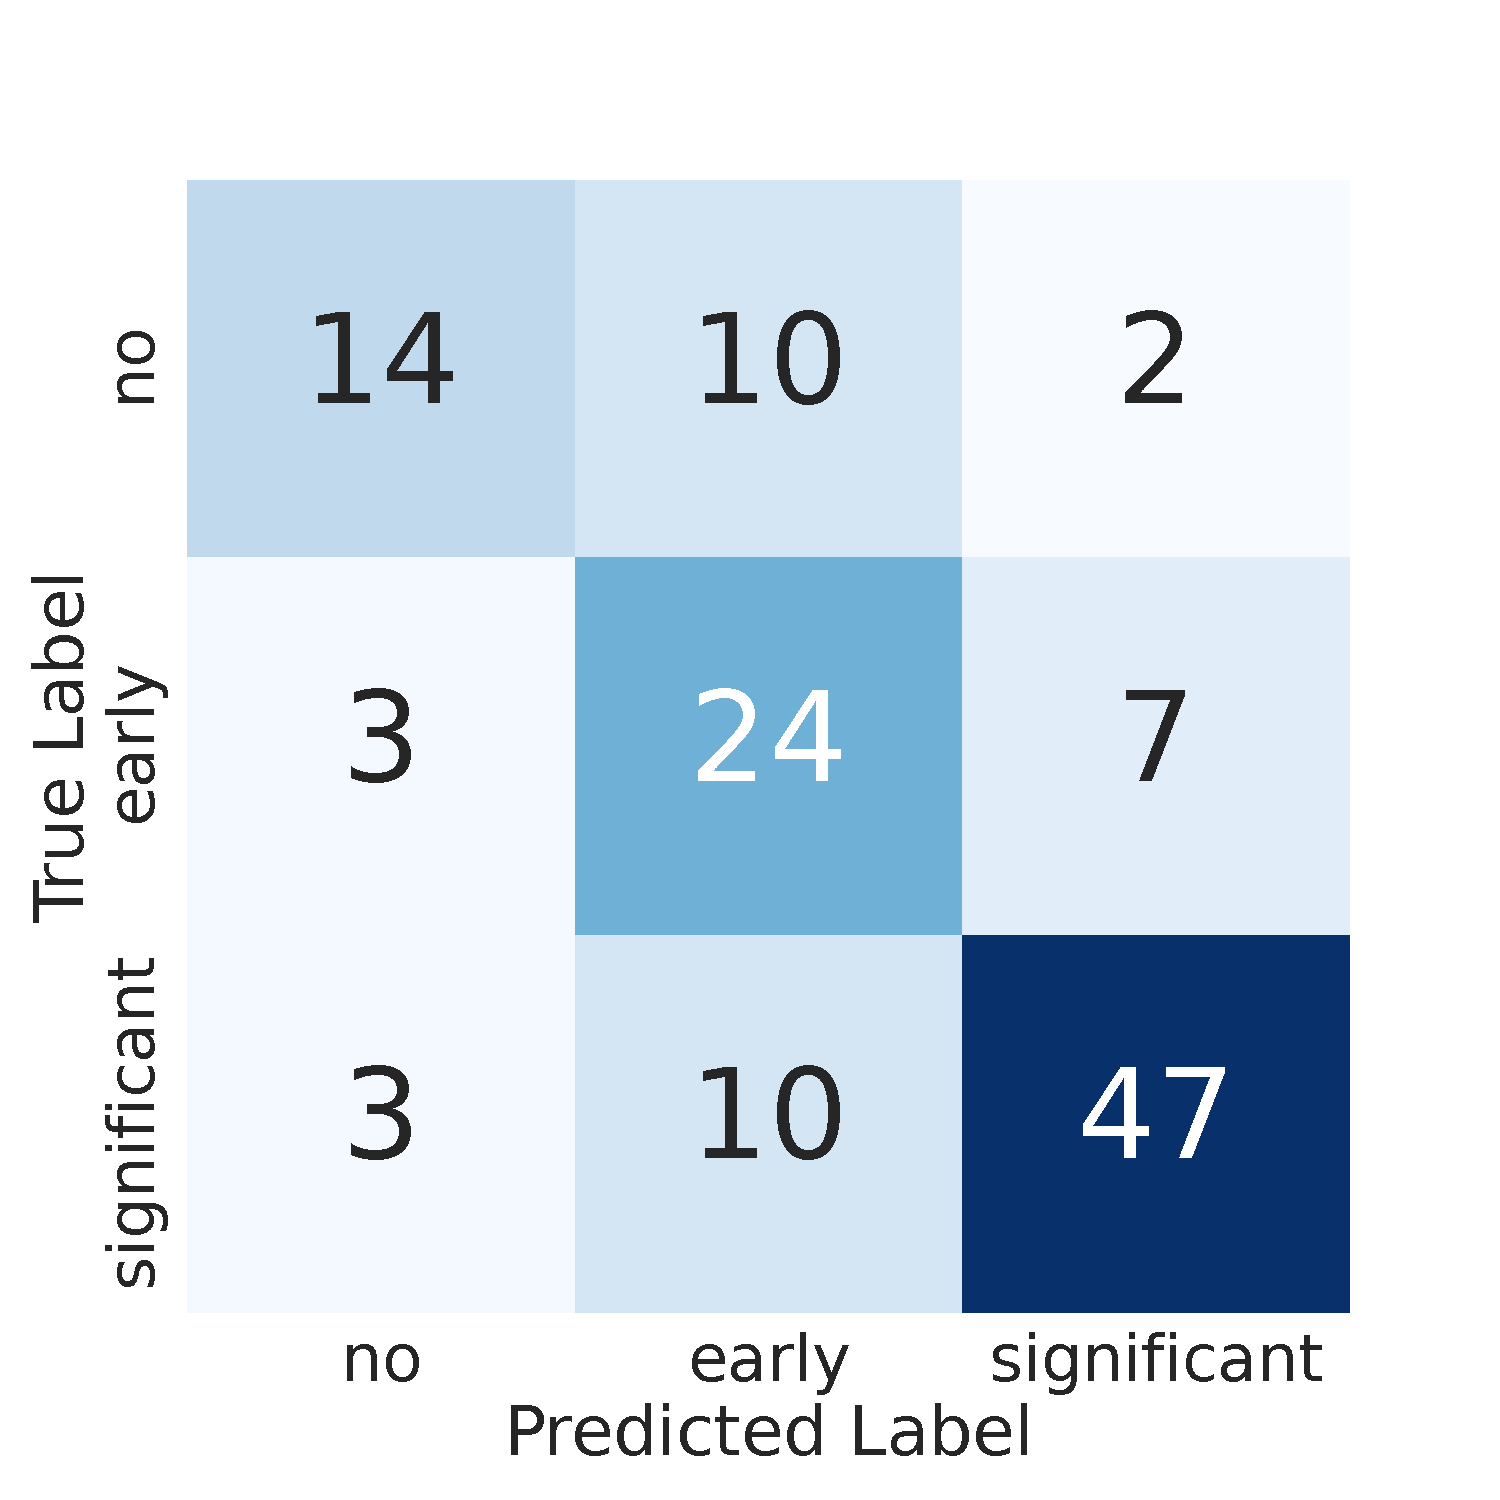
\includegraphics[width=\BW\textwidth]{figures/confusion_matrix/cropped_seed1/OffTheShelfDSMIL.pdf}
    &
    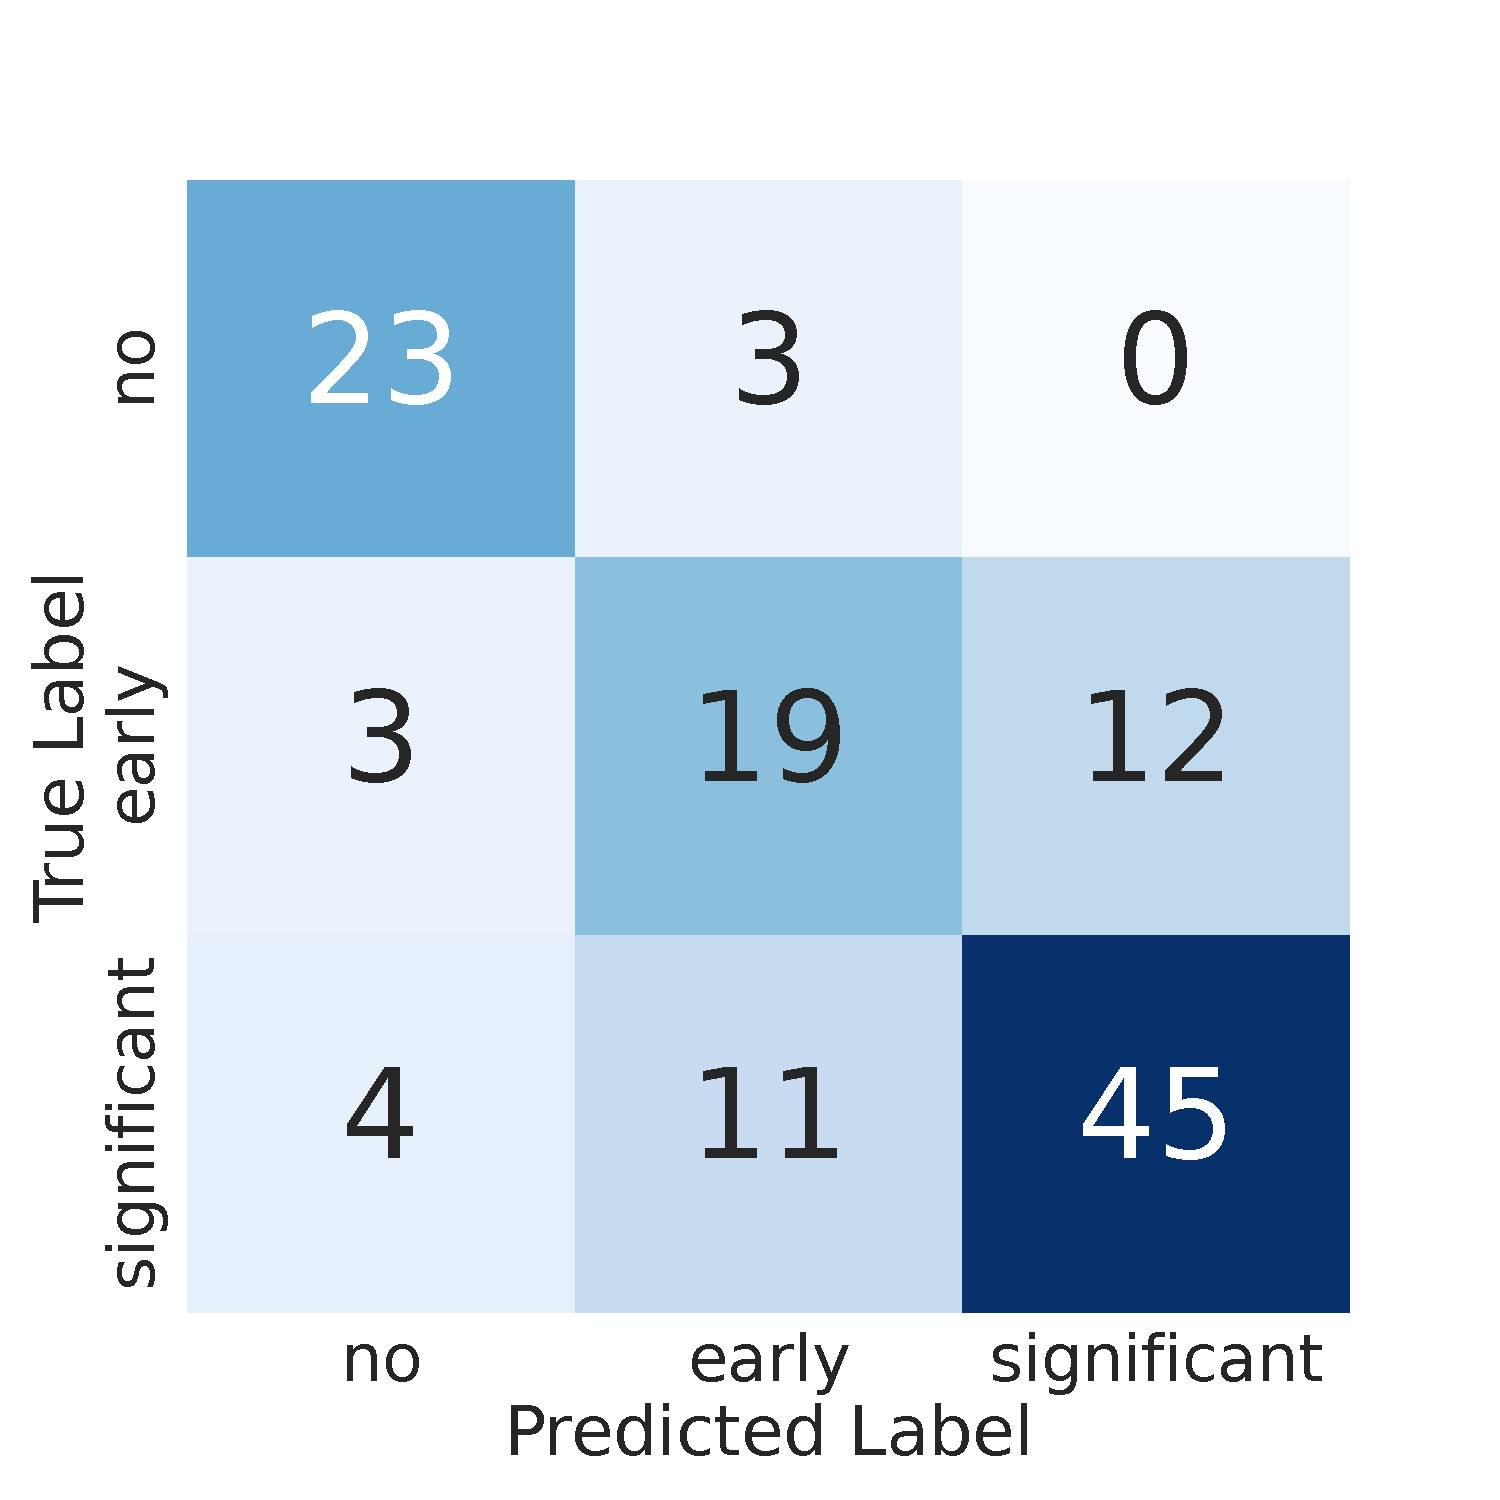
\includegraphics[width=\BW\textwidth]{figures/confusion_matrix/cropped_seed2/OffTheShelfDSMIL.pdf}
    \\
    {\rotatebox{90}{~~~~~~~~ SAMIL (ours)}}
    & 
    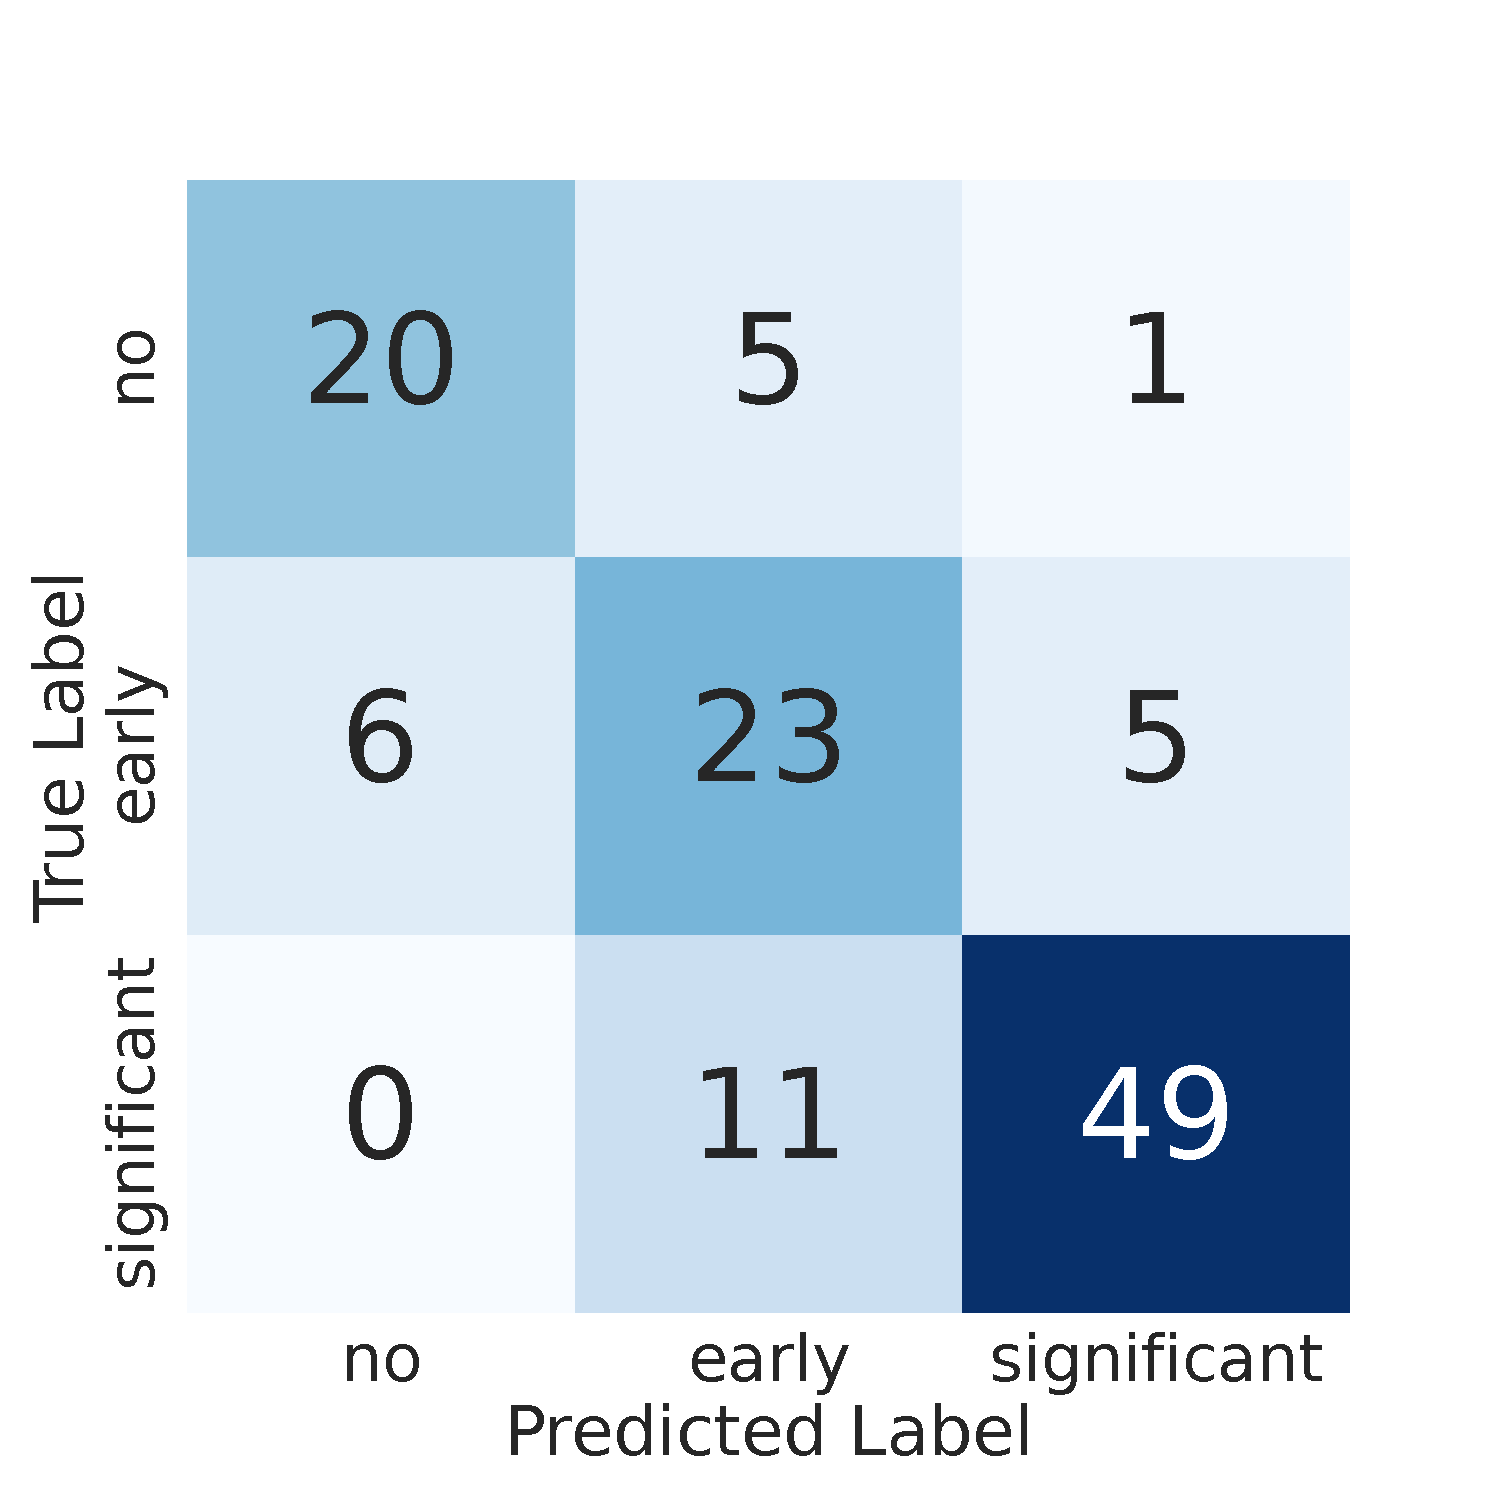
\includegraphics[width=\BW\textwidth]{figures/confusion_matrix/cropped_seed0/VRABMIL_WholeMILPretrain.pdf}
    &
    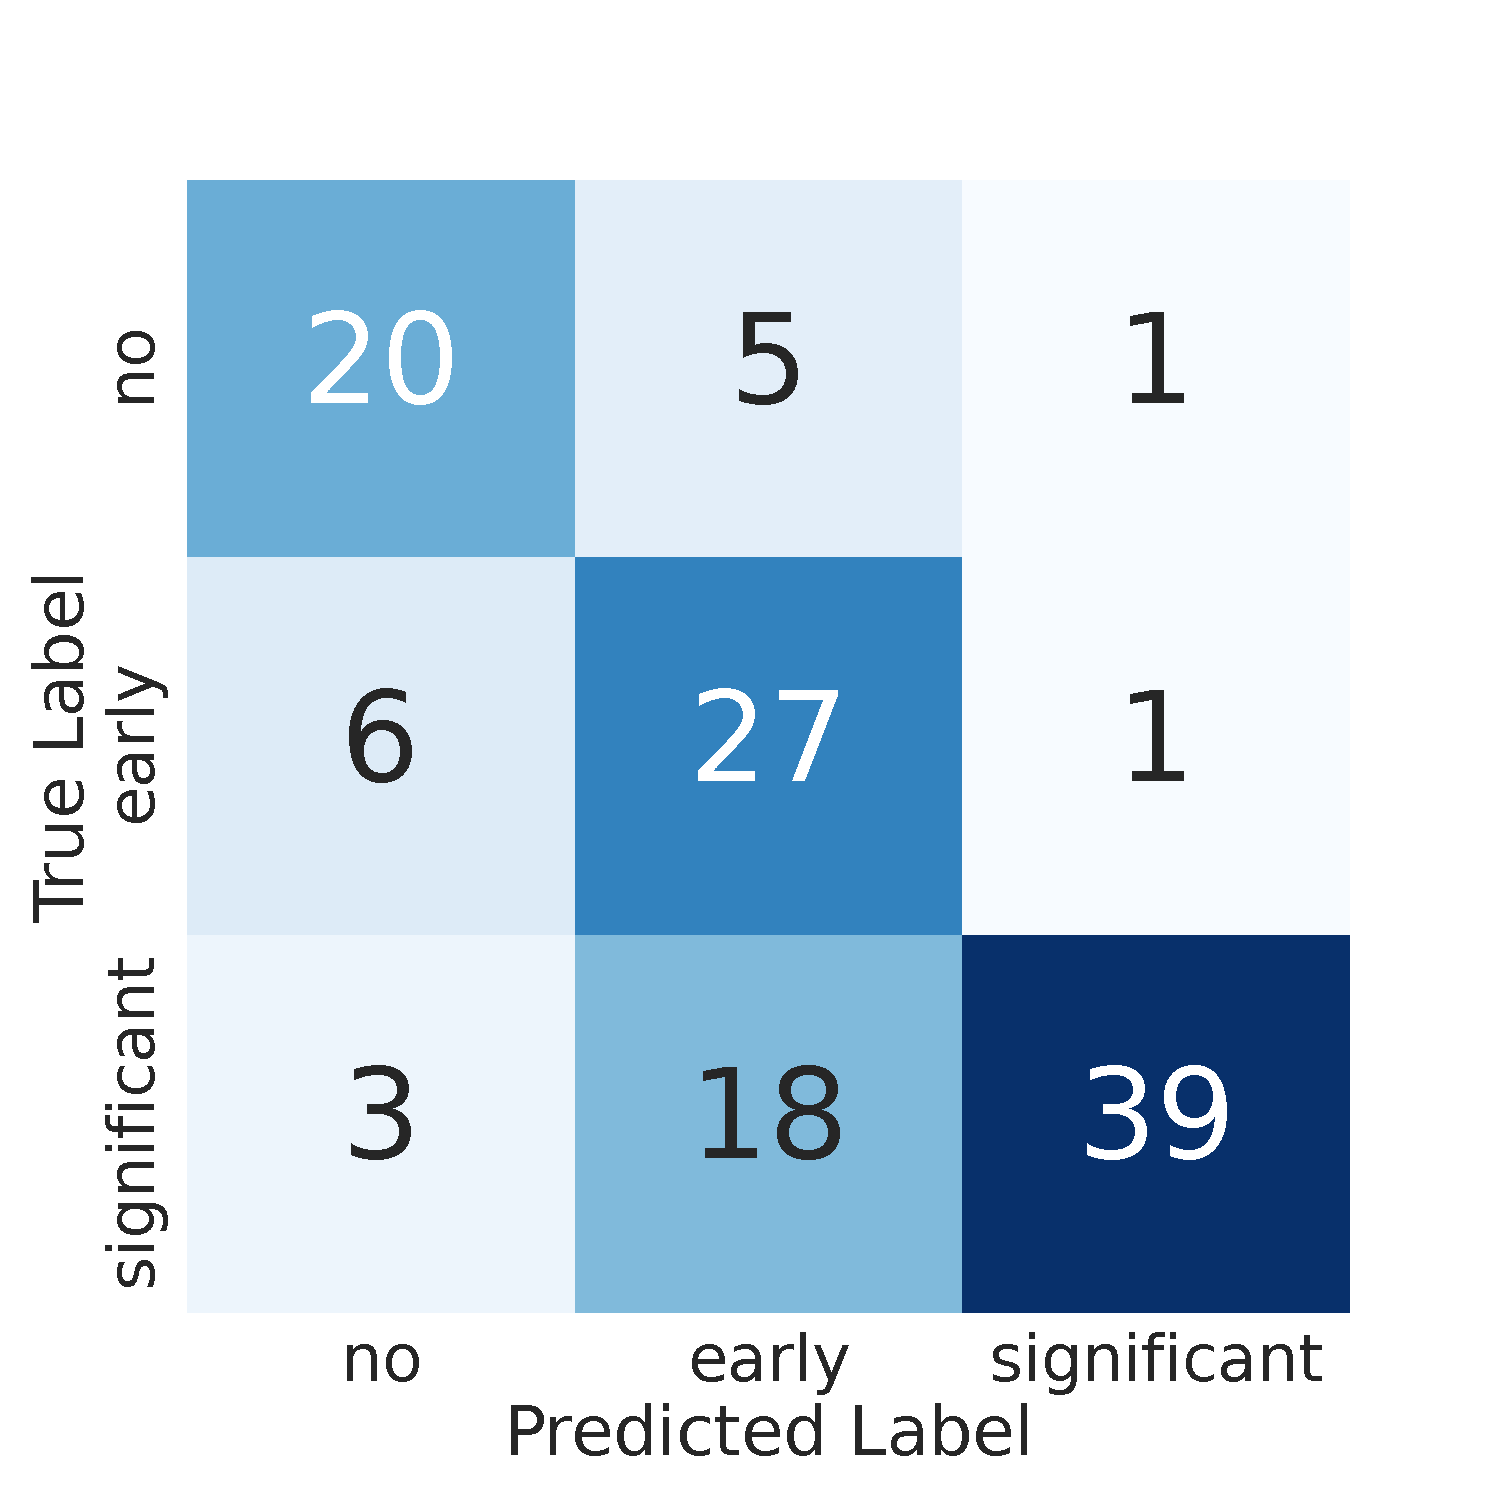
\includegraphics[width=\BW\textwidth]{figures/confusion_matrix/cropped_seed1/VRABMIL_WholeMILPretrain.pdf}
    &
    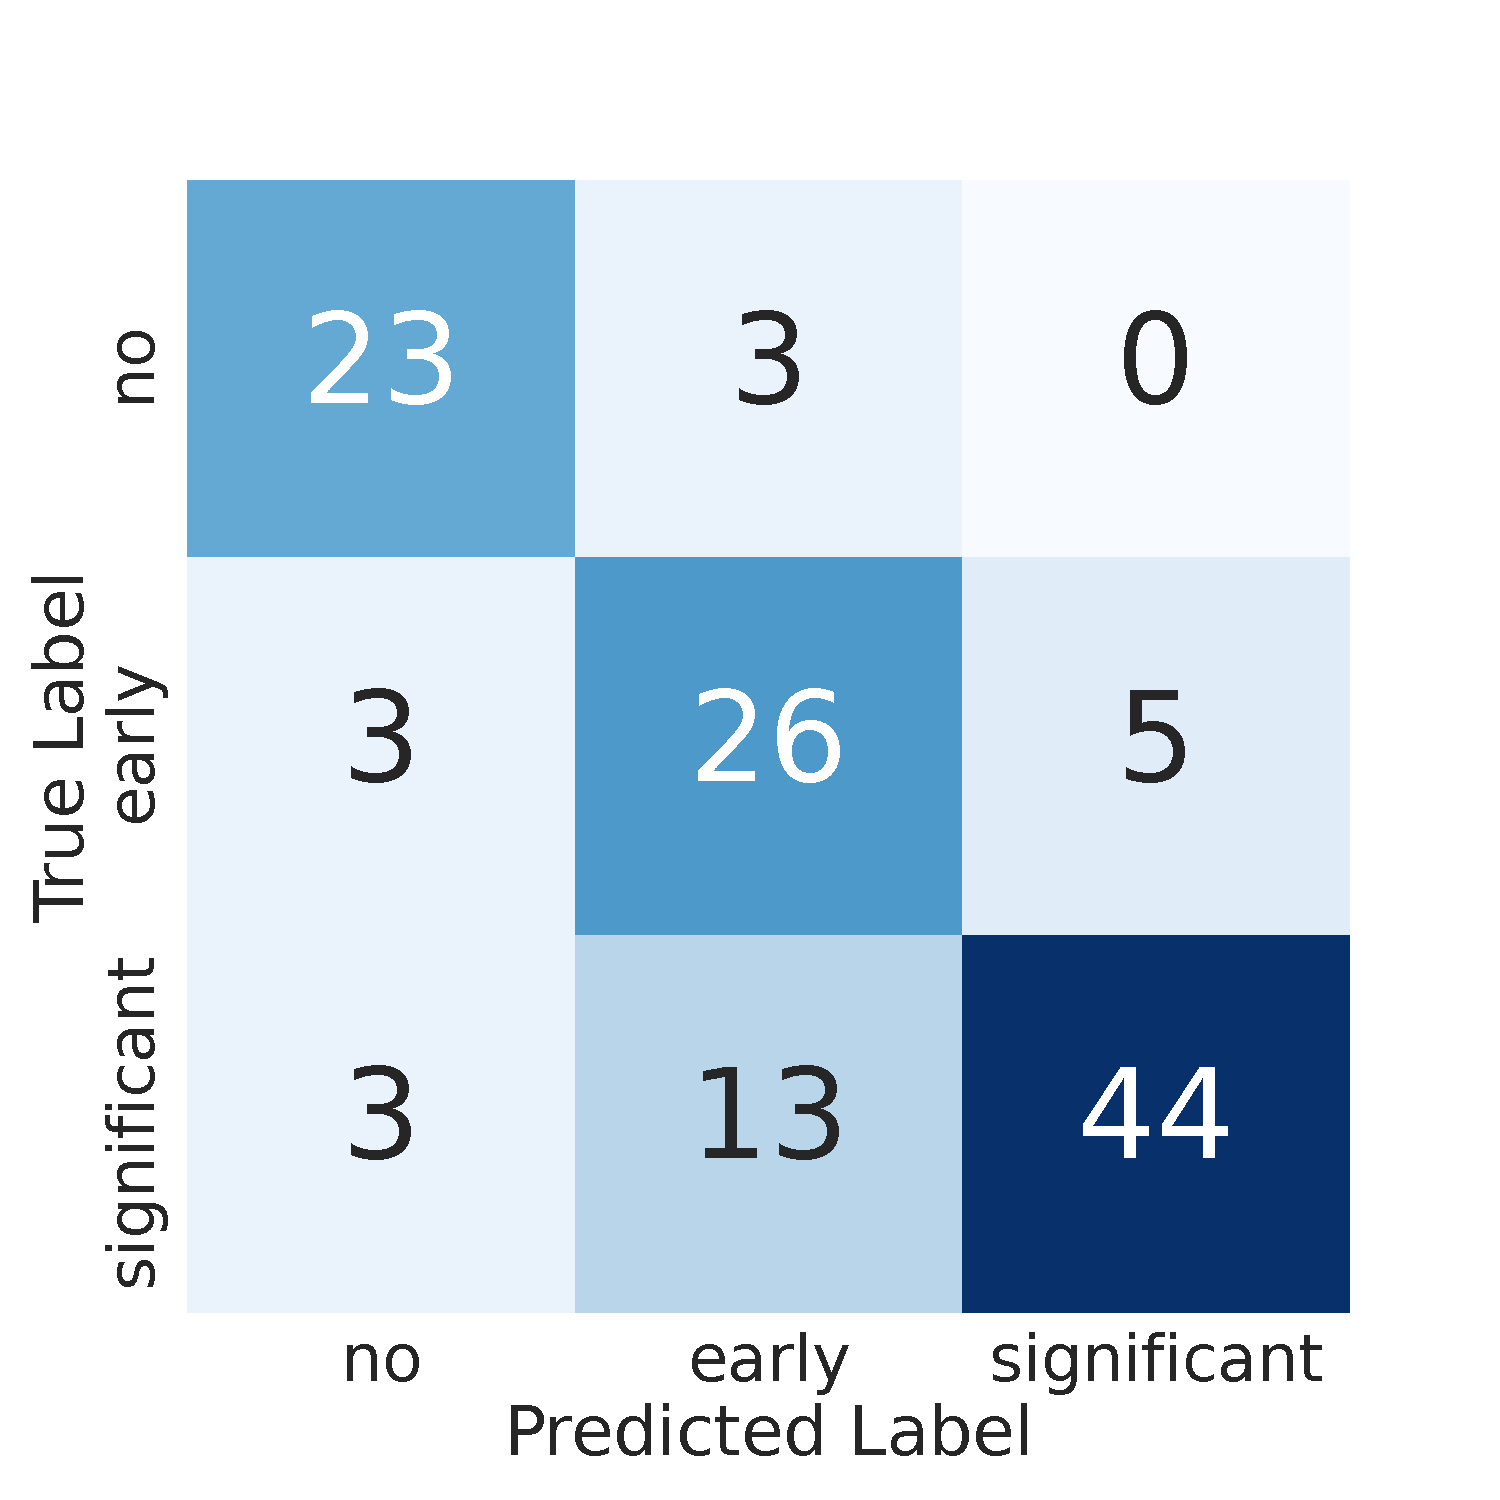
\includegraphics[width=\BW\textwidth]{figures/confusion_matrix/cropped_seed2/VRABMIL_WholeMILPretrain.pdf}
    \end{tabular}
    \vspace{-.5cm} %% WHITESPACE HACK
    \caption{Confusion matrices for the patient-level AS diagnosis classification, across three predefined train/test splits of TMED2.
     }
    \label{fig:confusion_matrix}
\end{figure}


\subsection{ROC for AS Screening Tasks}
\newcommand{\BWWW}{0.4}
\setlength{\tabcolsep}{0.1cm}
\begin{figure}[H]
\begin{tabular}{r c c c }
    & No vs Some AS & Early vs Significant AS & NoSignificant vs Significant AS
    \\
    {\rotatebox{90}{~~~~Split1}}
    & 
    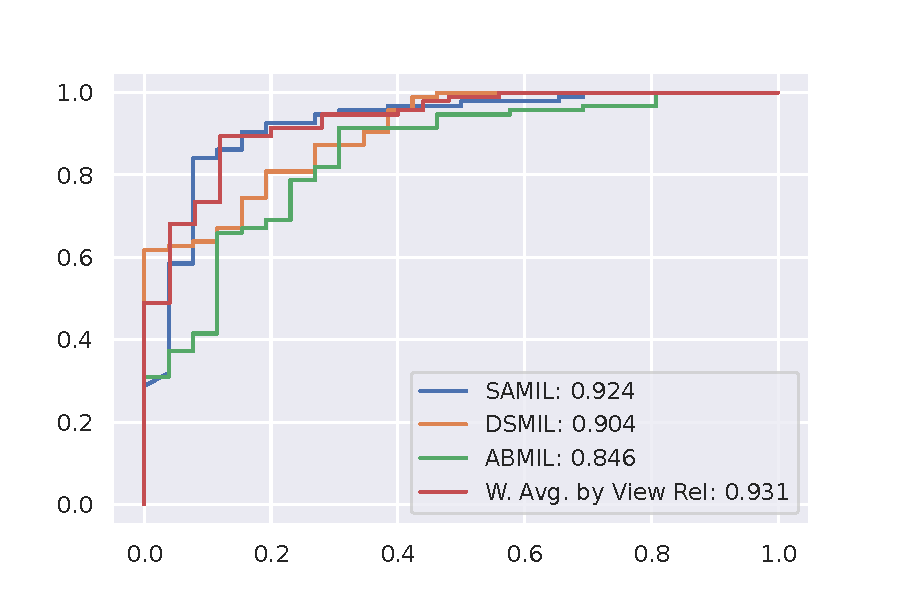
\includegraphics[width=\BWWW\textwidth]{figures/AUC_Analysis/data_seed0/NoASvsSomeAS_withDSMIL_DSMILupdatedseed0.pdf}
    &
    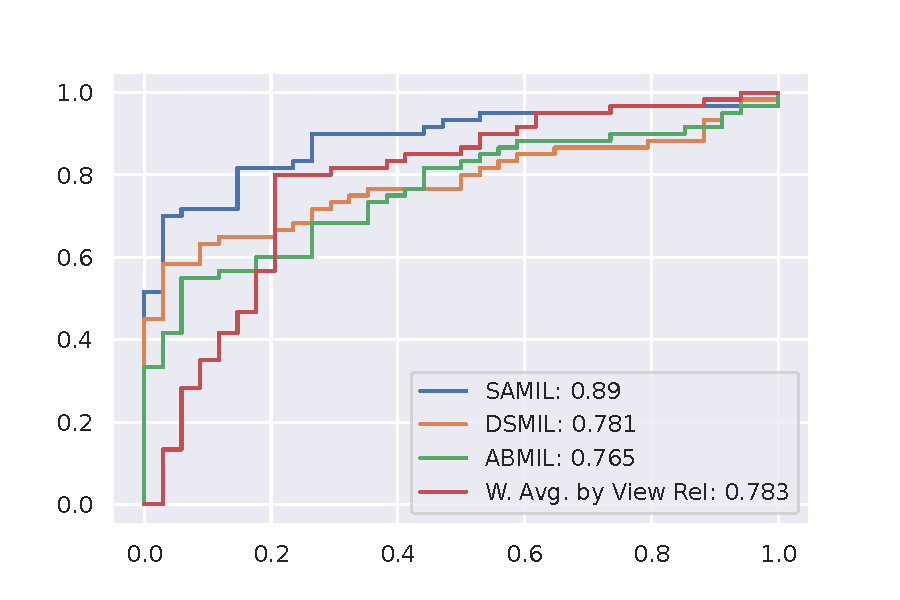
\includegraphics[width=\BWWW\textwidth]{figures/AUC_Analysis/data_seed0/EarlyASvsSignificantAS_withDSMIL_DSMILupdatedseed0.pdf}
    &
    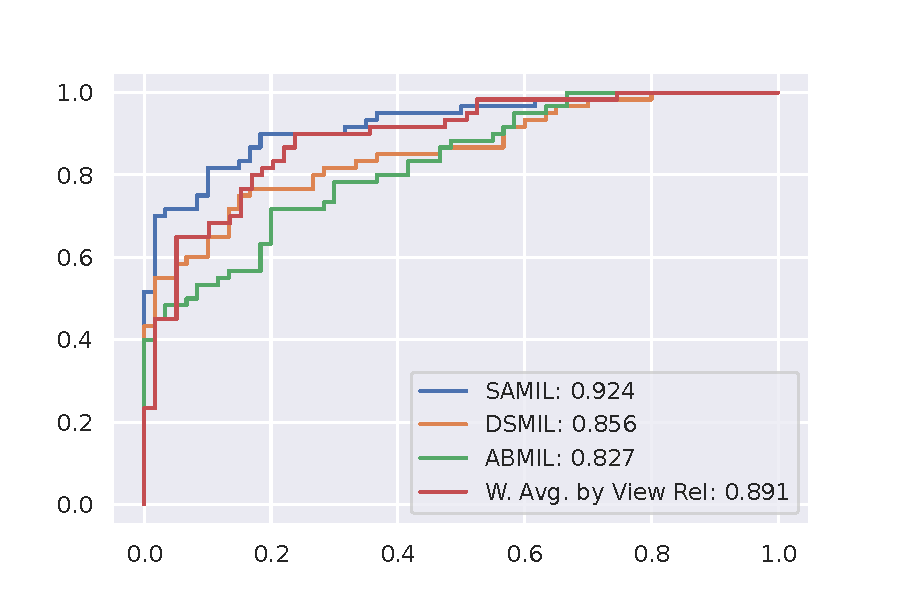
\includegraphics[width=\BWWW\textwidth]{figures/AUC_Analysis/data_seed0/SignificantASvsNoSignificantAS_withDSMIL_DSMILupdatedseed0.pdf}
    
    \\
    {\rotatebox{90}{~~~~Split2}}
    & 
    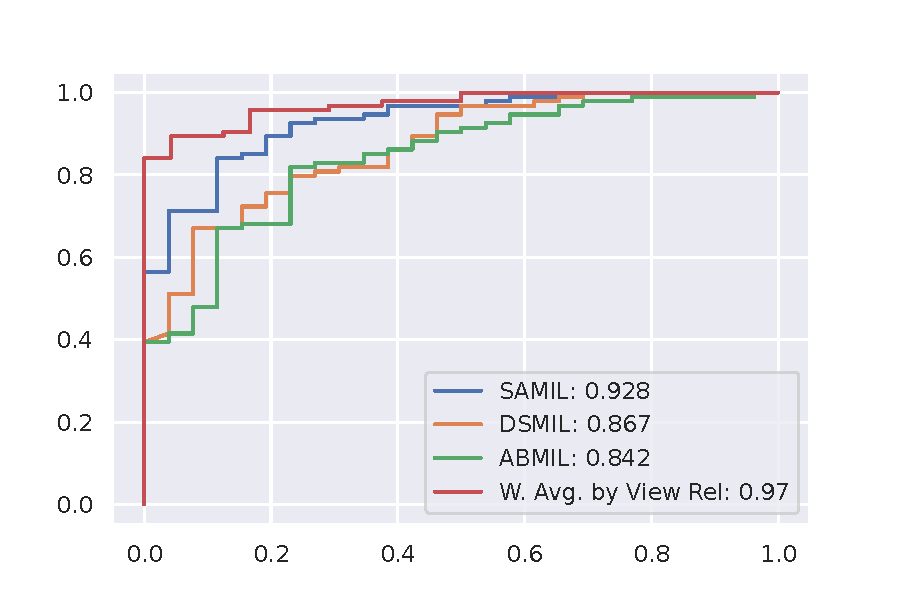
\includegraphics[width=\BWWW\textwidth]{figures/AUC_Analysis/data_seed1/NoASvsSomeAS_withDSMIL.pdf}
    &
    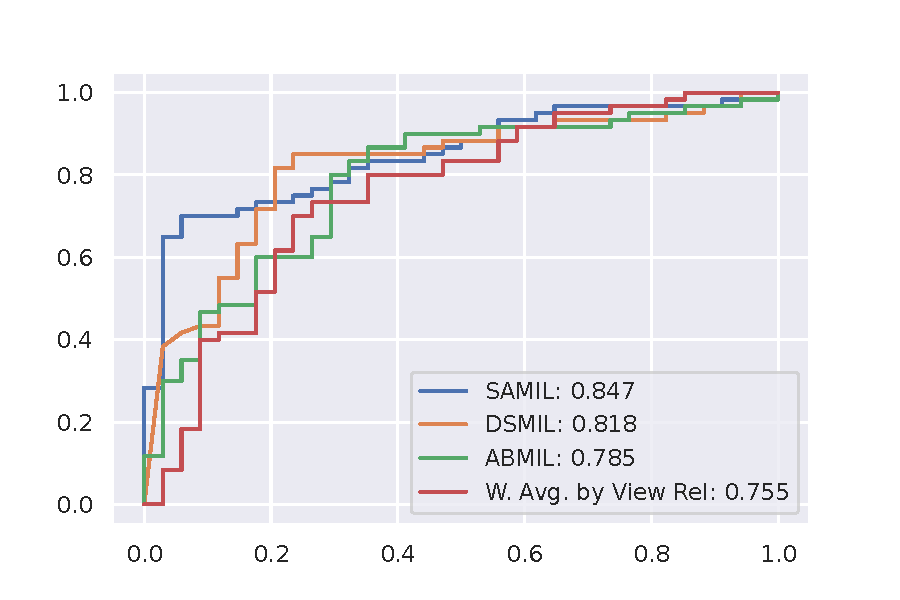
\includegraphics[width=\BWWW\textwidth]{figures/AUC_Analysis/data_seed1/EarlyASvsSignificantAS_withDSMIL.pdf}
    &
    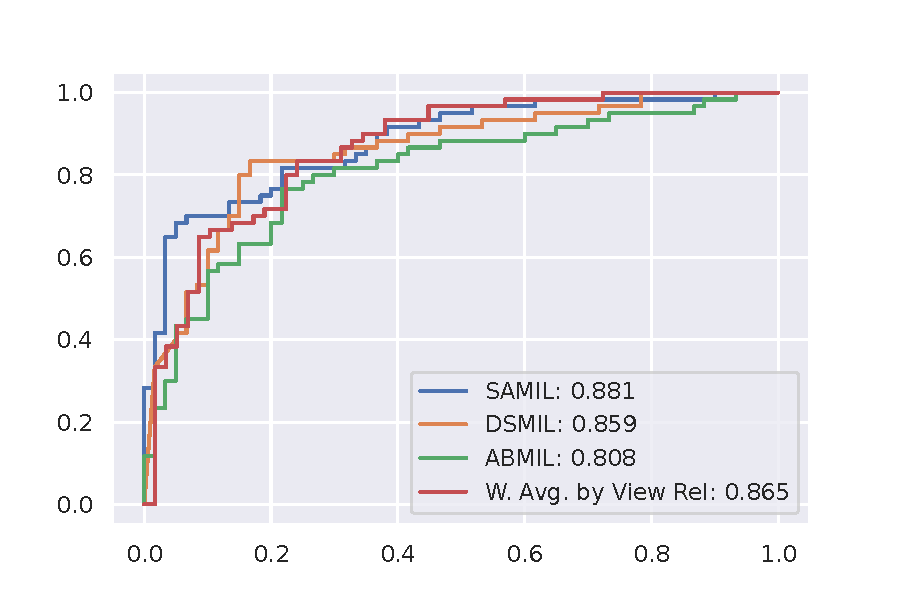
\includegraphics[width=\BWWW\textwidth]{figures/AUC_Analysis/data_seed1/SignificantASvsNoSignificantAS_withDSMIL.pdf}

    \\
    {\rotatebox{90}{~~~~Split3}}
    & 
    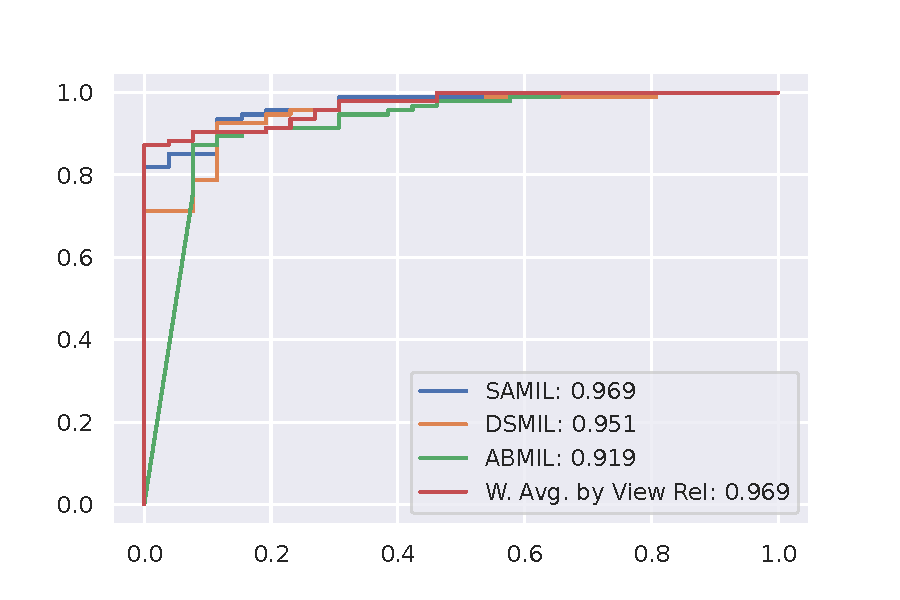
\includegraphics[width=\BWWW\textwidth]{figures/AUC_Analysis/data_seed2/NoASvsSomeAS_withDSMIL.pdf}
    &
    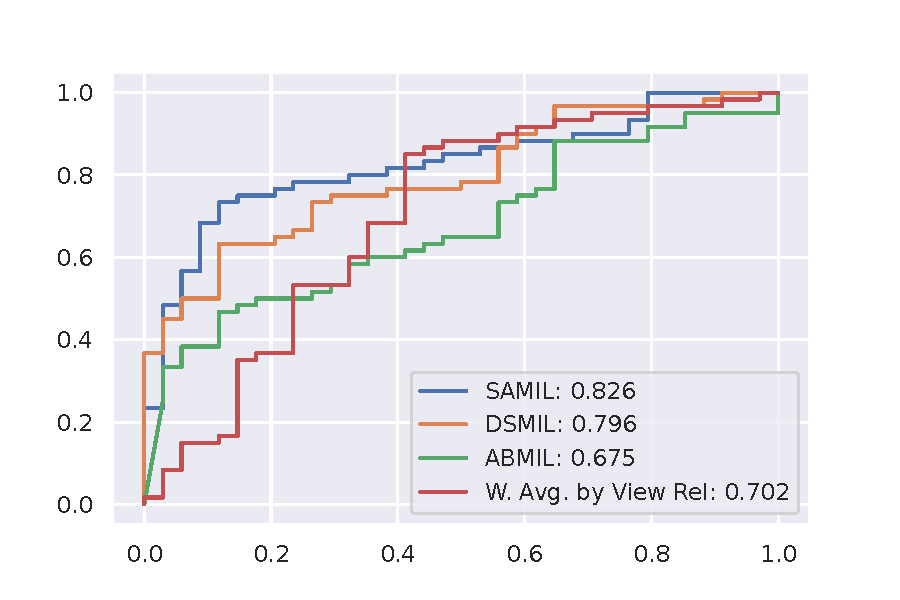
\includegraphics[width=\BWWW\textwidth]{figures/AUC_Analysis/data_seed2/EarlyASvsSignificantAS_withDSMIL.pdf}
    &
    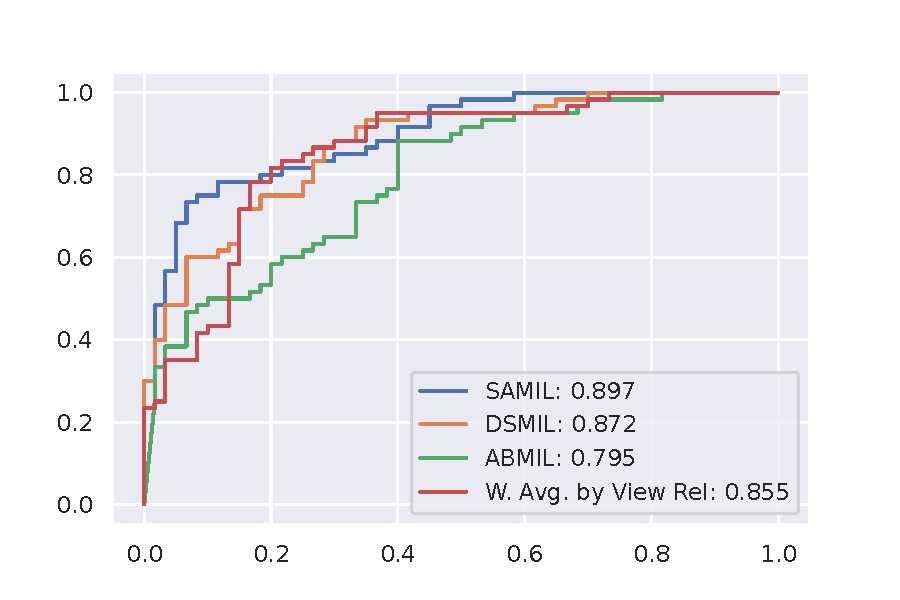
\includegraphics[width=\BWWW\textwidth]{figures/AUC_Analysis/data_seed2/SignificantASvsNoSignificantAS_withDSMIL.pdf}
    
    \end{tabular}	
    \caption{Diagnosis classification receiver operator curves. Showing results across three predefined train/test splits of TMED2 and three clinically relevant screening tasks.
     }
    \label{fig:TMED2_roc}
\end{figure}


\subsection{Attended Images by SAMIL and ABMIL}
\renewcommand{\BW}{0.18}
\setlength{\tabcolsep}{0.1cm}
% \begin{figure}[!h]
\begin{figure}[H]
\begin{tabular}{r c c c c c}
    \\
    {\rotatebox{90}{~~~~~~ABMIL}}
    & 
    \fcolorbox{green}{white}{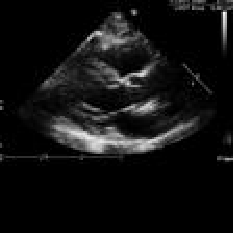
\includegraphics[width=\BW\textwidth]{figures/top_attended_images/2927484s1_OffTheShelfABMIL_top1_BVBO0SL1_0.pdf}}
    &
    \fcolorbox{green}{white}{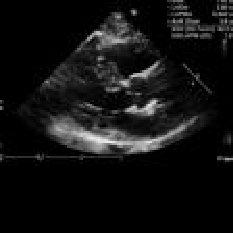
\includegraphics[width=\BW\textwidth]{figures/top_attended_images/2927484s1_OffTheShelfABMIL_top2_BVBO0SL0_0.pdf}}
    &
    \fcolorbox{green}{white}{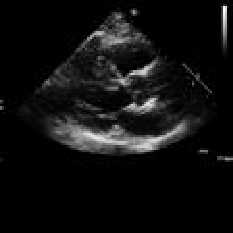
\includegraphics[width=\BW\textwidth]{figures/top_attended_images/2927484s1_OffTheShelfABMIL_top3_BVBO0SKQ_0.pdf}}
    &
    \fcolorbox{green}{white}{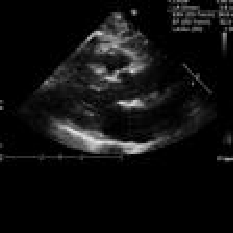
\includegraphics[width=\BW\textwidth]{figures/top_attended_images/2927484s1_OffTheShelfABMIL_top4_BVBO0SL2_0.pdf}}
    &
    \fcolorbox{green}{white}{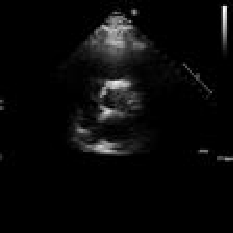
\includegraphics[width=\BW\textwidth]{figures/top_attended_images/2927484s1_OffTheShelfABMIL_top5_BVBO0SM0_0.pdf}}
    
    \\
    {\rotatebox{90}{~~~~~~~~~~~~ABMIL}}
     & 
    \fcolorbox{red}{white}{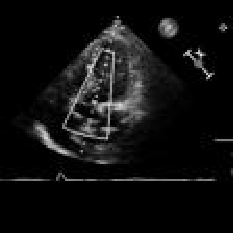
\includegraphics[width=\BW\textwidth]{figures/top_attended_images/2927484s1_OffTheShelfABMIL_top6_BVBO0SPG_1.pdf}}
    &
    \fcolorbox{red}{white}{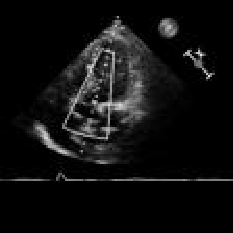
\includegraphics[width=\BW\textwidth]{figures/top_attended_images/2927484s1_OffTheShelfABMIL_top7_BVBO0SPF_1.pdf}}
    &
    \fcolorbox{red}{white}{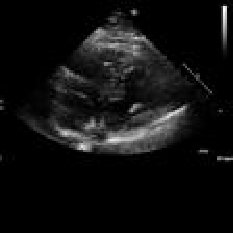
\includegraphics[width=\BW\textwidth]{figures/top_attended_images/2927484s1_OffTheShelfABMIL_top8_BVBO0SMX_0.pdf}}
    &
    \fcolorbox{red}{white}{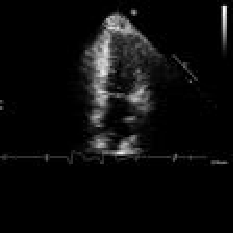
\includegraphics[width=\BW\textwidth]{figures/top_attended_images/2927484s1_OffTheShelfABMIL_top9_BVBO0SPV_0.pdf}}
    &
    \fcolorbox{red}{white}{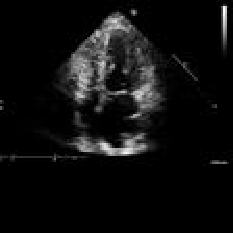
\includegraphics[width=\BW\textwidth]{figures/top_attended_images/2927484s1_OffTheShelfABMIL_top10_BVBO0SOT_0.pdf}}
    
    \\
    {\rotatebox{90}{~~~~~~~~~~~~SAMIL}}
     & 
    \fcolorbox{green}{white}{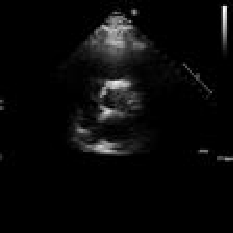
\includegraphics[width=\BW\textwidth]{figures/top_attended_images/2927484s1_SAMIL_top1_BVBO0SM0_0.pdf}}
    &
    \fcolorbox{green}{white}{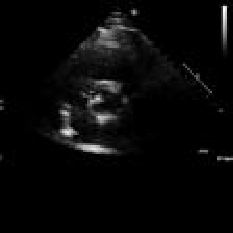
\includegraphics[width=\BW\textwidth]{figures/top_attended_images/2927484s1_SAMIL_top2_BVBO0SMM_0.pdf}}
    &
    \fcolorbox{green}{white}{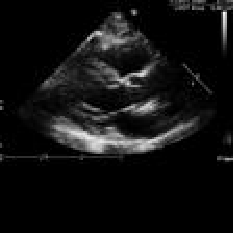
\includegraphics[width=\BW\textwidth]{figures/top_attended_images/2927484s1_SAMIL_top3_BVBO0SL1_0.pdf}}
    &
    \fcolorbox{green}{white}{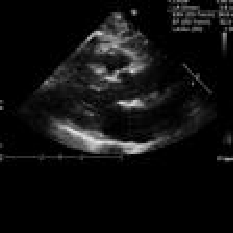
\includegraphics[width=\BW\textwidth]{figures/top_attended_images/2927484s1_SAMIL_top4_BVBO0SL2_0.pdf}}
    &
    \fcolorbox{green}{white}{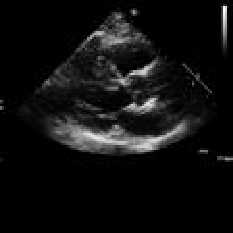
\includegraphics[width=\BW\textwidth]{figures/top_attended_images/2927484s1_SAMIL_top5_BVBO0SKQ_0.pdf}}
    
    \\
    {\rotatebox{90}{~~~~~~~~ SAMIL}}
     & 
    \fcolorbox{green}{white}{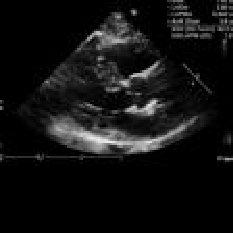
\includegraphics[width=\BW\textwidth]{figures/top_attended_images/2927484s1_SAMIL_top6_BVBO0SL0_0.pdf}}
    &
    \fcolorbox{green}{white}{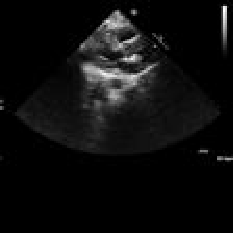
\includegraphics[width=\BW\textwidth]{figures/top_attended_images/2927484s1_SAMIL_top7_BVBO0SKM_0.pdf}}
    &
   \fcolorbox{green}{white}{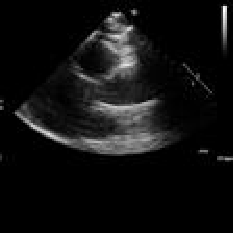
\includegraphics[width=\BW\textwidth]{figures/top_attended_images/2927484s1_SAMIL_top8_BVBO0SL6_0.pdf}}
    &
    \fcolorbox{green}{white}{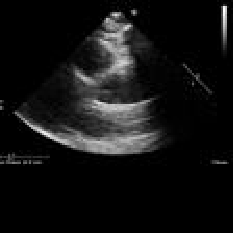
\includegraphics[width=\BW\textwidth]{figures/top_attended_images/2927484s1_SAMIL_top9_BVBO0SLB_0.pdf}}
    &
    \fcolorbox{green}{white}{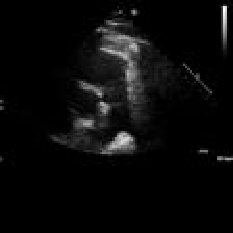
\includegraphics[width=\BW\textwidth]{figures/top_attended_images/2927484s1_SAMIL_top10_BVBO0SMD_0.pdf}}
    
    \end{tabular}	
    \caption{Showing top attended images for the first study in the test set. The top 2 rows show the top 10 attended images by ABMIL, bottom 2 rows show the top 10 attended images by SAMIL. Red box indicates the image is not a clinically relevant view for AS diagnosis.
     }
    \label{fig:top_attended_images}
\end{figure}

\section{Methods Supplement}
\subsection{Architecture}
\label{app:Architecture}
Below we report the architecture details for SAMIL. For feature extractor $f$, we use a simple stack of convolution layers as done in ABMIL~\citep{ilse2018attention}.
\begin{table}[!h] 
\centering 
\begin{tabular}{l}
~~~~~Feature Extractor $f$ \\
\midrule
Conv2d(3, 20, kernel=(5,5))\\
ReLU()\\
MaxPool2d(2, stride=2)\\
Conv2d(20, 50, kernel=(5,5))\\
ReLU()\\
MaxPool2d(2, stride=2)\\
Conv2d(50, 100, kernel=(5,5))\\
ReLU()\\
Conv2d(100, 200, kernel=(5,5))\\
ReLU()\\
MaxPool2d(2, stride=2)\\

\bottomrule
\end{tabular}
\caption{Details of Feature Extractor $f$}
\label{tab:Feature Extractor $f$}
\end{table} 
We used the same feature extractor $f$ shown in \ref{tab:Feature Extractor $f$} for SAMIL, ABMIL, Set Transformer and DSMIL.

The feature extractor $f$ maps each of the original images into 200 feature maps with smaller size. In practice, a MLP can be use (optional) to further process the flattened feature maps (also see Fig~\ref{fig:workflow_diagram}). We use the same MLP [Linear(32000, 500), ReLU(), Linear(500, 250), ReLU(), Linear(250, 500), ReLU()] for both SAMIL and ABMIL. For Set Transformer, we directly flattened the extracted feature maps and feed them to the Set Transformer's ISAB blocks. Please refer to original paper~\citep{lee2019set} for more details. For DSMIL, the extracted feature maps are flattened and projected to vectors of dimension 500 by a linear layer followed by ReLU, and then feed to its two streams. Please refer to original paper~\citep{li2021dual} for more details.

For the pooling layer $\sigma$, we use the same MLP architectures (shown in \ref{tab:attention_MLP}) for both the supervised attention branch and flexible attention branch in SAMIL. Note that this is also the same MLP architecture to learn attention weights in ABMIL.

\begin{table}[!h] 
\centering 
\begin{tabular}{l}
MLP learning attention weights \\
\midrule
Linear(500, 128)\\
Tanh()\\
Linear(128, 1)\\

\bottomrule
\end{tabular}
\caption{Details of MLP used to learn attention weights for SAMIL and ABMIL}
\label{tab:attention_MLP}
\end{table} 

For output layer $g$ both SAMIL and ABMIL use a simple linear layer (with softmax). Our experiments for DSMIL,  and Set Transformer are mainly based on the official open-source code from corresponding paper. Please refer to the original papers for more details on their $\sigma$ and $g$.




\subsection{View Classifier}
\label{app:ViewClassifier}
We train a view classifier for each of the three splits independently. We train the classifiers using a recently proposed semi-supervised learning method~\citep{huang2022fix} with Pi-model~\citep{laine2016temporal}. We used the view labeled images in each split's train set (as the labeled data) as well as the unlabeled set (as the unlabeled data). 

The view classifiers are trained to output probabilities of three category: PLAX, PSAX and Other. The view classifiers' performance is shown in \ref{tab:viewclassifier_performance}

\begin{table}[h]
\centering
\begin{tabular}{c|c|c|c}
Method & split1 & split2 & split3 \\
\hline
Fix-A-Step + Pi  & 97.20  & 98.14 & 98.00

\end{tabular}
\caption{Balanced accuracy on view classification. Showing view classification on TMED2 test set's view labeled images.}
\label{tab:viewclassifier_performance}
\end{table}

\paragraph{Backbone.} The view classifiers use Wide ResNet~\citep{zagoruyko2016wide} as backbone,  specifically, the ``WRN-28-2'' that has a depth 28 and width 2.

\paragraph{Training and Hyperparameters.} We train the view classifiers using SGD~\citep{robbins1951stochastic} as optimizer. We train the classifiers for 500 epochs, and retain the checkpoint that has maximum validation accuracy on the validation set. Hyperparameters used are reported below~\ref{tab:ViewClassifier hyperparameters}

\begin{table}[!htb]
\centering
\begin{tabular}{l|c|c|c}
Hyperparameter & split1 & split2 & split3 \\
\midrule
Labeled batch size & 64 & 64 & 64 \\
Unlabeled batch size & 64 & 64 & 64 \\
Learning rate & 0.0003 & 0.009 & 0.009 \\
Weight decay & 0.05 & 0.0005 & 0.0005 \\
Max consistency coefficient & 0.3 & 0.3 & 0.3 \\
Beta shape $\alpha$ & 0.5 & 0.5 & 0.5 \\
Unlabeled loss warmup schedule & linear & linear & linear \\
Learning rate schedule & cosine & cosine & cosine\\
\end{tabular}
\caption{Hyperparameters used for the view classifiers in each split.}
\label{tab:ViewClassifier hyperparameters}
\end{table}




\section{MIL Experiment Details}
\subsection{Details on Filter then Avg. Approach}
\label{App:Filter then Avg.}
To apply the Filter then Avg. approach proposed on TMED2, we follow closely the steps outlined in the paper ~\citet{holste2022automated,holste2022self}. We first use the same view classifiers that are used for SAMIL to prefilter images in the dataset, keeping only images that are predicted as PLAX. We then use a 2D ResNet18~\citep{he2016deep} to train the diagnosis classifier to classify each retained PLAX image as no AS, early AS or significant AS. In aggregation step, we average the AS predictions of all PLAX images in a study to obtain the study-level AS prediction. Note that author in ~\citep{holste2022self} uses a 3D ResNet18~\citep{tran2018closer} since their proprietary dataset consists of 3D videos while the open access TMED2 consists of 2D images. For the same reason, we are not able to directly use their self-superivsed training strategy that are proposed for 3D videos.

\subsection{Details on DeepSet}
\label{App:DeepSet}
DeepSet~\citep{zaheer2017deep} process each instance in the bag independently, and aggregate the processed feature embedding using simple pooling (mean or max). Fully connected layers are then used to map the aggregated feature embeddings into a bag prediction.

We perform the same hyperparameter search for DeepSet as shown below~\ref{App:Hyper}. However, we won't able to obtain any meaningful results, which suggest that problem of using multiple ultrasound images for AS diagnosis is too challenging for simple architecture like DeepSet.

\subsection{Training.} Our open source code (will be released after upon acceptance) uses PyTorch ~\citep{paszke2019pytorch}. For all methods compared, we use SGD~\citep{robbins1951stochastic} as optimizer. Each method is set to train for 2000 epochs, and early stop if validation performance does not increase for 200 consecutive epochs. Each training run uses one NVIDIA A100 GPU.

\subsection{Hyperparameter.} 
\label{App:Hyper}
We perform a grid search for each algorithm and each data split. From our preliminary experiments, we found that learning rate around 0.0005 and weight decay around 0.0001 is a good starting point. 

For DSMIL, ABMIL, Set Transformer, DeepSet and Filter then Avg, we search learning rate in [0.0003, 0.0005, 0.0008, 0.001, 0.003] and weight decay in [0.00001, 0.00003, 0.0001, 0.0003, 0.001]. SAMIL involves two additional hyperparameters, a temperature scaling term $\tau_{v}$ used in eq.~\ref{eq:L_SA}, and $\lambda_{SA}$ in eq.~\ref{eq:total_loss} that balance the supervised attention loss and the cross-entropy loss. For SAMIL, we search learning rate in [0.0005, 0.0008], weight decay in [0.0001, 0.001], $\tau_{v}$ in [0.1, 0.05, 0.03] and $\lambda_{SA}$ in [5, 15, 20]. Note that for ABMIL with gated attention, we did not search hyperparameters again, but directly use the corresponding best hyperparameter from its general attention version. Note that we perform same set of independent hyperparameter search for experiments on SAMIL with bag-level pretraining, image-level pretraining and without pretraining.

Final hyperparameter used are reported as follow:

% \begin{table}[!htb]
\begin{table}[H]
\centering
\begin{tabular}{l|c|c|c}
\multicolumn{4}{c}{SAMIL (with study-level SSL)} \\
Hyperparameter & split1 & split2 & split3 \\
\midrule
Learning rate & 0.0005 & 0.0008 & 0.0005 \\
Weight decay & 0.0001 & 0.001 & 0.001 \\
Temperature T & 0.1 & 0.1 & 0.05 \\
$\lambda_{SA}$ & 15.0 & 20.0 & 20.0 \\
Learning rate schedule & cosine & cosine & cosine\\
\end{tabular}
\caption{Hyperparameter settings for SAMIL across different data splits.}
\label{tab:SAMIL_hyper_nopretrain}
\end{table}

\begin{table}[!htb]
\centering
\begin{tabular}{l|c|c|c}
\multicolumn{4}{c}{DSMIL} \\
Hyperparameter & split1 & split2 & split3 \\
\midrule
Learning rate & 0.001 & 0.0008 & 0.0008 \\
Weight decay & 0.0001 & 0.00003 & 0.00001 \\
Learning rate schedule & cosine & cosine & cosine\\
\end{tabular}
\caption{Hyperparameter settings for DSMIL across different data splits.}
\label{tab:DSMIL_hyper}
\end{table}

\begin{table}[!htb]
\centering
\begin{tabular}{l|c|c|c}
\multicolumn{4}{c}{ABMIL} \\
Hyperparameter & split1 & split2 & split3 \\
\midrule
Learning rate & 0.0008 & 0.0005 & 0.0008 \\
Weight decay & 0.0001 & 0.00005 & 0.00005 \\
Learning rate schedule & cosine & cosine & cosine\\
\end{tabular}
\caption{Hyperparameter settings for ABMIL across different data splits.}
\label{tab:ABMIL_hyper}
\end{table}

\begin{table}[!htb]
\centering
\begin{tabular}{l|c|c|c}
\multicolumn{4}{c}{Set Transformer} \\
Hyperparameter & split1 & split2 & split3 \\
\midrule
Learning rate & 0.0010 & 0.0008 & 0.0008 \\
Weight decay & 0.00003 & 0.0001 & 0.00001 \\
Learning rate schedule & cosine & cosine & cosine\\
\end{tabular}
\caption{Hyperparameter settings for Set Transformer across different data splits.}
\label{tab:SetTransformer_hyper}
\end{table}


\begin{table}[!htb]
\centering
\begin{tabular}{l|c|c|c}
\multicolumn{4}{c}{Filter then Avg.} \\
Hyperparameter & split1 & split2 & split3 \\
\midrule
Learning rate & 0.003 & 0.001 & 0.003 \\
Weight decay & 0.00003 & 0.00001 & 0.00001 \\
Learning rate schedule & cosine & cosine & cosine\\
\end{tabular}
\caption{Hyperparameter settings for Filter then Avg. across different data splits.}
\label{tab:Filter then Avg._hyper}
\end{table}



\section{Self-supervised Pretraining}
\label{app:SSL_Pretraining}
Our implementation is based on the official code from MoCo~\citep{he2020momentum,chen2020improved}. For image-level contrastive learning, we set learning rate to 0.06, weight decay to 0.0005, batch size to 512, size of queue to 4096, momentum m to 0.99, softmax temperature to 0.1. For bag-level contrastive learning, we set learning rate to 0.00015 (following the linear Scaling Relu~\citep{goyal2017accurate}, which is also recommended by MoCo's author), weight decay to 0.0005, batch size to 1, size of queue to 4096, momentum m to 0.99, softmax temperature to 0.1. Note that we did not tune hyperparameters for the self-supervised pretraining. 

We train the model using the train set as well as the unlabeled set for both image-level and bag-level contrastive learning. The model is set to train for 200 epochs, with early stopping monitored by knn protocol on the validation set. The early stopping patience is set to 20.

\paragraph{projection head $\psi$.} The projection head is a two-layer MLP with the structure [Linear(500, 500), ReLU(), Linear(500, 128)]. The projection head is used to project the image or bag representation to a latent space where the contrastive loss is applied. The projection head is discarded after training following the convention from ~\citep{chen2020improved,chen2020simple}.

\section{Additional Related Work}
\label{app:relatedworks}
\paragraph{Classic approaches.}
% Numerous studies have been conducted on MIL even before the  ``deep learning era'' \footnote[1]{It is usually refered to 2012 when AlexNet achieved a significant improvement in image recognition accuracy over previous methods in the ImageNet Large Scale Visual Recognition Challenge}. 
% Numerous studies on MIL have been conducted even prior to the advent of deep learning. 
Examples of classic MIL methods includes iARP~\citep{dietterich1997solving}, 
Diverse Density~\citep{maron1997framework}, 
Citation-kNN~\citep{wang2000solving}, MI-Kernels~\citep{zhang2001dd}, MI/mi-SVM~\citep{andrews2002support}, mi-Graph ~\citep{zhou2009multi}, MILBoost~\citep{zhang2005multiple}, GPMIL~\citep{kim2010gaussian}, among others. 



\end{document}
